%%%%%%%%%%%%%%%%%%%%%%%%%%%%%%%%%%%%%%%%%%%
% File      : res
% Author    : th202608@pleiades068.intra.cea.fr
% Date      : 15 oct. 2012
% Directory : /home/th202608/codes/tfel/tests/Broyden/
%%%%%%%%%%%%%%%%%%%%%%%%%%%%%%%%%%%%%%%%%%%

\documentclass[rectoverso,pleiades,pstricks,leqno,anti,projet]{texmf/note_technique_2010}

%\usepackage[dvips]{graphicx}
%\usepackage[dvips,breaklinks]{hyperref}

\usepackage{texmf/mathematiques}
\usepackage{texmf/mecanique}
\usepackage{texmf/couleurs}
\usepackage{texmf/presentation}

\usepackage{pst-plot}
\usepackage{array}
\usepackage{subfigure}
\usepackage{relsize}
\usepackage{multind}

%% one column index
%\makeatletter
%\def\printindex#1#2{\section*{#2}
%\addcontentsline{toc}{section}{#2}
%\@input{#1.ind}}
%\makeatother

\usepackage[frenchb]{babel}

\newcommand{\pleiades}{\texttt{pleiades}}
\newcommand{\tfel}{\texttt{tfel}}
\newcommand{\mfront}{\texttt{mfront}}
\newcommand{\cyrano}{\texttt{cyrano}}
\newcommand{\castem}{\texttt{Cast3M}}
\newcommand{\pycastem}{\texttt{pyCast3M}}
\newcommand{\umat}{\texttt{umat}}
\newcommand{\sirius}{\texttt{sirius}}
\newcommand{\fortran}{\texttt{fortran}}

\newcommand{\mkey}[1]{\index{mkeys}{#1@\symbol{64}#1}{\texttt{@#1}}}

%c from texinfo.tex
\def\ifmonospace{\ifdim\fontdimen3\font=0pt }

%c C plus plus
\def\cpp{%
\ifmonospace%
    C++%
\else%
    C\kern-.1667em\raise.30ex\hbox{\smaller{++}}%
\fi%
\spacefactor1000 }

\newcommand{\varcpp}[1]{\texttt{#1}}

\newcommand{\sigmaH}{\ensuremath{\sigma_{H}}}

\newcommand{\nbzrc}{$NbZrC$}
\newcommand{\upuc}{$\paren{U,Pu}C$}
\newcommand{\sic}{$SiC$}

\newcommand{\cea}{CEA}
\newcommand{\windows}{\href{http://www.microsoft.com/france/windows/default.mspx}{\texttt{Windows}}}
\newcommand{\linux}{\href{http://www.kernel.org/}{\texttt{linux}}}
\newcommand{\excel}{\href{http://www.microsoft.com/france/office/2007/programs/excel/overview.mspx}{\texttt{Microsoft Office Excel}}}

\newcommand{\debutpas}[1]{\ensuremath{\left.#1\right|_{t}}}
\newcommand{\milieupas}[1]{\ensuremath{\left.#1\right|_{t+\theta\, \Delta\, t}}}
\newcommand{\finpas}[1]{\ensuremath{\left.#1\right|_{t+\Delta\, t}}}
\newcommand{\demipas}[1]{\ensuremath{\left.#1\right|_{t+\frac{\Delta\, t}{2}}}}

\newcommand{\code}[1]{
  \psframebox[linecolor=ceaorange,shadow=true,blur=true]{
    \begin{minipage}[htbp]{1.0\linewidth}
      \ttfamily\scriptsize #1
    \end{minipage}
  }
}

%%%%%%%%%%%%%%%%%%%%%%%%%%%%%%%%%%%%%%%%%%%%%%%%%%%%%%%%%%%%%%%%%%%%%%%%%%%%%%%
%%	Fichier	   : Champs
%%	Auteur     : th202608@pleiades052.intra.cea.fr
%%	Date       : 13 dc 2010
%%	Rpertoire : /home/th202608/documents/notes/2011/LicosPresentation/
%%%%%%%%%%%%%%%%%%%%%%%%%%%%%%%%%%%%%%%%%%%%%%%%%%%%%%%%%%%%%%%%%%%%%%%%%%%%%%%

% Initialisation des variables par defaut
\centre{CAD}
%% 2005 : \centre{Direction du CEA/Cadarache}
%% mais pas utilise !
\centrenom{Cadarache}
\direction{DEN}
\directionnom{Direction de l'\'Energie Nucl\'eaire}
\departement{DEC}
\departementnom{D\'epartement d'\'Etudes des Combustibles}
\service{SESC}
\servicenom{Service d'\'Etudes et de Simulation du comportement des Combustibles}
\batimentservice{151}
\telephoneservice{23 66}
\faxservice{47 47}

\emetteur{M.~Bauer}

%% ajout pour le modele 2005 :
\directiontitre{Direction de l'\'Energie Nucl\'eaire}
\departementtitre{D\'epartement d'\'Etudes des Combustibles}
\servicetitre{Service d'\'Etudes et de Simulation du comportement des Combustibles}

\laboratoire{LSC}
% \laboratoiretitre{Laboratoire de simulation du comportement des combustibles}
% \batiment{151}
% \telephone{38 62}
% \fax{29 49}
% \mail{sesclsc@drncad.cea.fr}

\approbateur{R.~Masson}


\auteurs{T.~Helfer, V.~Blanc, J.~Julien}
\redacteur{T.~Helfer}
\verificateur{}
\approbateur{R.~Masson}
\emetteur{E.~Touron}

\titre{Le générateur de code \mfront{}~: gestion pérenne, robuste,
  efficace et évolutive des connaissances matériau dans la plateforme
  \pleiades{}}

\date{2013}
% \numero{12-014}
\indice{0}
% \dateversion{09/2012}
\numeroaffaire{A-SICOM-A1-01}
\domaine{DEN/DISN/SIMU}
% \accords{tripartite}
% \clients{AREVA - EDF}
\programmerecherche{SICOM}
\classification{DO}
\motsclefs{
  \mfront{} - \pleiades{}
}

% \codebarre{images/code_barre}
% \diffusionexterne{
% {EDF/R\&D}              & O. Marchand     & 1 & Diffusion par\\
% {EDF/R\&D}              & P. Vasseur      & 1 & courriel     \\
% {EDF/R\&D/MMC}          & P. Ollar         & 1 & \\
% {EDF/R\&D/MMC/CPM}      & N. Prompt       & 1 & \\
%                         & N. Barnel       & 1 & \\
% {EDF/R\&D/MMC/CPM}      & G. Thouvenin    & 1 & \\
%                         & R. Largenton    & 1 & \\
%                         & C. Petry        & 1 & \\
% EDF/SEPTEN              & N. Waeckel      & 1 & \\
%                         & P. Hemmerich    & 1 & \\
%                         & H. Billat       & 1 & \\
%                         & C. Bernaudat    & 1 & \\
% AREVA NP/LA DEFENSE     & L. Catalani     & 1 & \\
%                         & L. Brunel       & 1 & \\
% AREVA NP/LYON           & P. Melin        & 1 & \\
%                         & V. Bessiron     & 1 & \\
%                         & C. Garnier      & 1 & \\                           
%                         & V. Garat        & 1 & \\
%                         & F. Arnoux       & 1 &
% }

\diffusioninterne{
}

% \signatures{-0.}{-39.2}{0.12}{images/signatures.eps}

\stylebib{texmf/bibtex/fr-insa}
\fichierbib{Bibliographie}

%%% Local Variables: 
%%% mode: latex
%%% TeX-master: "utilisation."
%%% End: 


\resumecea{

  \mfront{} est un générateur de code dédiée aux connaissances
  matériau~:
  \begin{itemize}
    \item les propriétés matériau~;
    \item les lois de comportement~;
    \item les modèles~;
  \end{itemize}
  
  Les objectifs sont, dans chaque cas~:
  \begin{itemize}
    \item de proposer un fichier d'entrée clair se focalisant
    sur l'{\em information physique}~;
    \item de ne demander qu'un {\em minimum} de connaissance
    informatique à l'utilisateur~;
    \item de générer des bibliothèques matériau {\em numériquement
      optimisée}, en particulier pour les lois de comportement~;
    \item de favoriser un dialogue \og~\oe{}cuménique~\fg entre
    les différentes applications de l'utilisateur.
  \end{itemize}
}

\makeindex{general}
\makeindex{mkeys}

\begin{document}

\clearpage
\newpage
\section{Introduction}

\paragraph{Utilisation de \mfront{} dans \cyrano{}}

Un effort de développement a été fait pour faciliter l'introduction
d'une loi de comportement mécanique dans \cyrano{} en utilisant le
formalisme de appels externes utilisé par \mfront{}\footnote{Il s'agit
d'une modification de l'interface \umat{} que nous avons proposé pour
permettre l'appel de lois de comportement mécanique dans des
bibliothèques externes. Auparavant une recompilation partielle de
\castem{} était nécessaire pour ajouter une loi. Outre la relative
complexité de cette recompilation pour un utilisateur final, cette façon
de procéder était incompatible avec l'utilisation faite de \castem{} par
les applications \pleiades{} via l'interface
\pycastem~\cite{t.06:_implan}.}.

\paragraph{Utilisation de \mfront{} au DER/SESI}

\clearpage
\newpage
\section{Présentation générale}

\mfront{} est un générateur de code~: partant d'un fichier contenant les
informations physiques et numériques utiles, \mfront{} génère un code
source \cpp{}.

Le fichier \mfront{} présente un certain nombre de directives
introduites par une arobase @.

\subsection{Notion d'analyseur}

Les connaissances matériaux supportées par \mfront{} sont classées en
trois catégories~:
\begin{itemize}
  \item les propriétés matériau~;
  \item les lois de comportement mécanique~;
  \item les modèles.
\end{itemize}

\mfront{} utilise la notion d'analyseur pour proposer une solution
adaptée à la connaissance considérée. Il existe par exemple plusieurs
analyseurs pour les lois de comportement mécanique~: certains de ces
analyseurs permettent de traiter toutes les lois de comportement avec un
formalisme d'intégration particulier et certains sont dédiées à un type
de loi particulier.

Dans la version présentée de \mfront{}, les analyseurs suivants sont
disponibles~:
\begin{itemize}
  \item l'analyseur {\tt Material\-Law} qui traite de propriétés
  matériau. La section~\ref{MaterialProperty} lui est consacrée~;
  \item l'analyseur \texttt{DefaultParser} qui permet de traiter tous
  types de lois de comportements~;
  \item l'analyseur \texttt{RungeKutta} qui propose la résolution d'une
  loi de comportement mécanique quelconque à l'aide de l'une des
  méthodes de \nom{Runge-Kutta}. Les méthodes disponibles sont des
  méthodes d'ordre \(2\) et \(4\) sans contrôle d'erreur et des méthodes
  correcteur prédicteur de type \(\pfrac{4}{2}\) ou \(\pfrac{5}{4}\)
  avec adaptation du pas de temps~;
  \item l'analyseur \texttt{IsotropicMisesCreep} qui gère exclusivement
  les lois de comportement mécanique viscoplastique isotrope de la
  forme~:
  \[
  \dot{p} = f\paren{\sigmaeq}
  \]
  où \(\dot{p}\) la vitesse viscoplastique équivalente et où
  \(\sigmaeq\) est la contrainte équivalente au sens de \nom{Von-Mises}.
  La direction d'écoulement est donnée par la condition de normalité.
  Une intégration implicite est effectuée. Cette intégration nécessite
  de préciser la dérivée \(\derivtot{f}{\sigmaeq}\)~;
  \item l'analyseur \texttt{IsotropicStrainHardeningMisesCreep} qui gère
  exclusivement les lois de comportement mécanique viscoplastique
  isotrope de la forme~:
  \[
  \dot{p} = f\paren{\sigmaeq,p}
  \]
  où \(\dot{p}\) la vitesse viscoplastique équivalente et où
  \(\sigmaeq\) est la contrainte équivalente au sens de \nom{Von-Mises}.
  La direction d'écoulement est donnée par la condition de normalité.
  Une intégration implicite est effectuée. Cette intégration nécessite
  de préciser les dérivées \(\deriv{f}{\sigmaeq}\) et \(\deriv{f}{p}\)~;
  \item l'analyseur \texttt{IsotropicPlasticMisesFlow} qui gère
  exclusivement les lois de comportement mécanique plastique isotrope de
  la forme~:
  \[
  f(\sigmaeq,p)\leq 0 \quad\quad \dot{p}\geq 0 \quad\quad
  f(\sigmaeq,p)\,\dot{p} = 0
  \]
  où \(p\) est la déformation plastique cumulée et où \(\sigmaeq\) est
  la contrainte équivalente au sens de \nom{Von-Mises}. La direction
  d'écoulement est donnée par la condition de normalité. Une intégration
  implicite est effectuée. Cette intégration nécessite de préciser les
  dérivées \(\deriv{f}{\sigmaeq}\) et \(\deriv{f}{p}\)~;
  \item l'analyseur \texttt{MultipleIsotropicMisesFlows} qui gère une
  combinaison arbitraire d'écoulements des trois types précédents. Les
  différents écoulements sont supposés non couplés.
  \item l'analyseur \texttt{Implicit} qui propose la résolution d'une
  loi de comportement mécanique quelconque à l'aide d'une intégration
  implicite. La méthode de résolution retenue pourra être ou un
  algorithme de \nom{Newton-Raphson} ou deux versions de l'algorithme de
  \nom{Broyden}~;
  \item l'analyseur \texttt{Model} qui permet de traiter des modèles.
\end{itemize}

La directive \mkey{Parser}, traditionnellement placé en tête du fichier
\mfront{} bien que cela ne soit pas nécessaire, est utilisée pour
décrire quel analyseur utilisé.

\subsection{Notion d'interface}

Les connaissances matériau ont été écrites pour être indépendantes du
code cible et favorisé leurs réutilisation dans des contextes logiciels
variés.

Pour cela, \mfront{} propose la notion d'interface~: le code source
généré dépend de l'interface choisie par l'utilisateur et cherche à
s'intégrer au mieux dans le contexte logiciel cible et à en tirer le
meilleur parti.

L'illustration la plus forte de cette notion d'interface est donnée par
les propriétés matériau qui propose par défaut différentes interfaces~:
\begin{itemize}
  \item l'interface \texttt{c} pour une utilisation dans des codes
  écrits dans ce language~;
  \item l'interface \texttt{fortran} pour une utilisation dans des codes
  écrits dans ce language~;
  \item l'interface \cpp{} pour une utilisation dans des codes
  écrits dans ce language~;
  \item l'interface \texttt{castem} pour une utilisation dans le code
  aux éléments finis \castem{}.~;
  \item l'interface \texttt{python} pour une utilisation dans des codes
  écrits dans ce language~;
  \item l'interface \texttt{gnuplot} pour une visualisation des courbes
  d'évolution des propriétés matériau en fonction de leur paramètres~;
\end{itemize}

\paragraph{Ajout d'interfaces} Il est possible de rajouter dynamiquement
de nouvelles interfaces par l'utilisation de la variable d'environnement
{\tt MFRONT\textunderscore{}\-ADDITIONAL\textunderscore{}\-LIBRARIES}
qui doit désigner une liste de librairies automatiquement chargées au
démarrage de \mfront{} \footnote{Ce mécanisme est utilisé par exemple
  par l'architecture \pleiades{} pour générer l'interface {\tt pleiades}
  aux propriétés matériau, interface qui évolue avec les versions de
  l'architecture.}.

Ce mécanisme permet donc de créer des interfaces sans modifier
\mfront{}.

\subsection{Noms de glossaire}

\subsection{Utilisation de librairies externes}

Les différents connaissances matériau sont écrites en \cpp{}. L'un des
intérêts de ce choix est de permettre l'utilisation de librairies
écrites dans des langages divers (\cpp{}, \texttt{c}, \texttt{fortran},
\ldots).

L'utilisation de ces librairies externes est décrites dans le paragraphe
suivant. Un cas particulier, celui des propriétés matériau écrites en
\mfront{} est ensuite traité.

\subsubsection{Librairies écrites dans d'autres langages}

L'utilisation de librairies extraites dans d'autres langages se fait
essentiellement à l'aide de deux mots clés~:
\begin{itemize}
  \item la directive \mkey{Includes} qui permet de déclarer des lignes
  de codes \cpp{} introduites en tête des fichiers générés. Ces lignes
  sont donnés dans un bloc commençant par une accolade ouvrante
  \texttt{\{} et se terminant par une accolade fermante \texttt{\}}. Le
  nom de cette directive est due au fait que ces instructions se
  résument généralement à une suite d'inclusions de fichiers d'entête
  par le mot clé \texttt{\#include} du préprocesseur \cpp{}.
  \item la directive \mkey{Link} est utilisée pour lier les librairies
  générées à des librairies externes. La directive \mkey{Link} est
  suivie d'une chaîne de caractère (entre doubles quotes) contenant des
  instructions à fournir à l'éditeurs de liens. L'utilisation des
  doubles quotes, inhabituelle dans la syntaxe \mfront{}, permet
  l'utilisation de caractères spéciaux.
\end{itemize}

\subsubsection{Appel aux propriétés matériau}

Les propriétés matériau jouent un rôle particulier car elles n'ont de
sens que relativement à une loi de comportement ou à un modèle. Par
ailleurs, des propriétés matériau peuvent liées. Par exemple, pour un
matériau dont le comportement mécanique est basé sur une loi
d'élasticité linéaire isotrope, le module d'\nom{Young} \(E\), le
coefficient de \nom{Poisson} \(\nu\) et le module de cisaillement \(G\)
sont reliés par~:
\[
\nu=\Frac{E}{2\,G}-1
\]

Afin de minimiser la duplication du code (et donc le risque d'erreur),
il est naturel que les différentes connaissances matériau puissent
utiliser des propriétés matériau définies par ailleurs.

Nous avons introduit la directive \mkey{MaterialLaw} pour traiter ces
cas.

\subsection{Directives communes à l'ensemble des analyseurs}

Nous décrivons dans ce paragraphe différentes directives communes à
l'ensemble des analyseurs.

\paragraph{La directive \mkey{Parser}} La directive \mkey{Parser} permet
de préciser l'analyseur utilisé. Cette directive est suivie du nom de
l'analyseur à utiliser et d'un point virgule.

\paragraph{La directive \mkey{Material}} La directive \mkey{Material}
précise le nom du matériau auquel se réfère la connaissance matériau. Ce
mot clé est suivi du nom du matériau et d'un point virgule. Ce nom de
matériau est généralement utilisé pour construire le nom des fonctions
ou des classes générées, il est donc soumis à certaines restrictions~:
un nom de matériau ne peut commencer par un chiffre et ne peut contenir
que des lettres alphabétiques ou des chiffres. Le nom du matériau peut
également être utilisé pour construire le nom de la librairie générée.

Cette information est optionnelle.

\paragraph{La directive \mkey{Description}} La directive
\mkey{Description} permet de donner de documenter le fichier \mfront{}.
Cette documentation est donnée dans un bloc commençant par une accolade
ouvrante \texttt{\{} et se terminant par une accolade fermante
\texttt{\}}. Elle doit idéalement contenir la référence d'où est
extraite la connaissance matériau traitée, les éventuelles adaptations
faites et le cadre d'utilisation.

Cette information est optionnelle.

\paragraph{La directive \mkey{Author}} Le mot clé \mkey{Author} donne le
nom de la personne qui a écrit le fichier \mfront{}. Ce mot clé est
suivi du nom jusqu'à ce qu'un point virgule soit rencontré.

Cette information est optionnelle.

\paragraph{La directive \mkey{Date}} Le mot clé \mkey{Date} donne la
date d'écriture du fichier \mfront{}. Ce mot clé est suivi de cette
date jusqu'à ce qu'un point virgule soit rencontré.

Cette information est optionnelle.

\paragraph{La directive \mkey{Library}} La directive spécifie le nom de
la librairie générée.

Cette information est optionnelle.

\paragraph{La directive \mkey{Includes}} La directive \mkey{Includes}
permet de déclarer des lignes de codes \cpp{} introduites en tête des
fichiers générés. Ces lignes sont donnés dans un bloc commençant par une
accolade ouvrante \texttt{\{} et se terminant par une accolade fermante
\texttt{\}}

Le nom de cette directive est due au fait que ces instructions se
résument généralement à une suite d'inclusions de fichiers d'entête par
le mot clé \texttt{\#include} du préprocesseur \cpp{}.

\paragraph{La directive \mkey{Link}} La directive \mkey{Link} est
utilisée pour lier les librairies générées à des librairies externes.

La directive \mkey{Link} est suivie d'une chaîne de caractère (entre
doubles quotes) contenant des instructions à fournir à l'éditeurs de
liens. L'utilisation des doubles quotes permet l'utilisation de
caractères spéciaux.



\subsection{Gestion de la compilation}

\clearpage
\newpage
\section{Propriétés matériaux}
\label{sec:MaterialProperty}

Les propriétés matériau sont l'un des éléments de connaissance
essentiel des matériaux. 

\subsection{Généralités}

Une propriété matériau est supposée dépendre de manière univoque des
valeurs actuelles d'un ensemble de variables d'état thermodynamique du
matériau. Ainsi, définir une propriété matériau revient à donner la
liste de ces variables d'état et la relation fonctionnelle qui permet
de la calculer, cette relation fonctionnelle étant souvent une
corrélation basée sur des mesures expérimentales.

\subsection{Catégorie des variables}

\paragraph{Bornes} Les variables d'états peuvent posséder des bornes
intrinsèques~: une température ne peut être négative, une porosité
supérieure à \(1\). Ces bornes intrinsèques sont dénommées dans la
suite \og~bornes physiques~\fg. Par ailleurs, la corrélation définissant
la propriété matériau a souvent été établie sur certain domaine~:
les limites de ce domaine expérimental seront dénommées
\og~bornes de validité~\fg (de la corrélation). 

\subsection{Interfaces disponibles} Les interfaces disponibles par
défaut pour cet analyseur sont~:
\begin{itemize}
  \item l'interface \texttt{c} pour une utilisation dans des codes
  écrits dans ce language~;
  \item l'interface \texttt{fortran} pour une utilisation dans des codes
  écrits dans ce language~;
  \item l'interface \texttt{c++} pour une utilisation dans des codes
  écrits dans ce language~;
  \item l'interface \texttt{castem} pour une utilisation dans le code
  aux éléments finis \castem{}. L'utilisation de cette interface a été
  décrite ailleurs~\cite{helfer07:_utilis}. Une utilisation directe de
  la librairie générée nécessite une version modifiée de \castem{}
  utilisée et maintenue au sein de la plateforme \pleiades{}.
  L'utilisation dans la version officielle est possible, mais il faut
  passer par une modification de la méthode {\tt compute} et une
  recompilation partielle de \castem{}~;
  \item l'interface \texttt{python} pour une utilisation dans des codes
  écrits dans ce language~;
  \item l'interface \texttt{gnuplot} pour une visualisation des courbes
  d'évolution des propriétés matériau en fonction de leur paramètres~;
\end{itemize}

\paragraph{Autres interfaces} D'autres interfaces peuvent être ajoutées
dynamiquement à \mfront{}. Pour cela, il suffit de définir une variable
d'environnement nommée {\tt
  MFRONT\textunderscore{}\-ADDITIONAL\textunderscore{}\-LIBRARIES} qui
doit désigner une liste de librairies automatiquement chargées au
démarrage\footnote{Ce mécanisme est utilisé par exemple par
  l'architecture \pleiades{} pour générer l'interface {\tt pleiades} aux
  propriétés matériau, interface qui évolue avec les versions de
  l'architecture.}.

\begin{table}[htbp]
  \centering
  \begin{tabular}[htbp]{|l|l|l|}
    \cline{2-3}
    \multicolumn{1}{c|}{\mbox{}} & \multicolumn{2}{c|}{Nom de la bibliothèque générée} \\
    \hline
    Interface & sous \windows{} & sous \linux{} \\
    \hline
    \hline
    \texttt{c}        & libMaterialLaw.dll       & libMaterialLaw.so    \\
    \hline
    \texttt{c++}      & libCppMaterialLaw.dll    & libCppMaterialLaw.so \\
    \hline
    \texttt{castem}   & libCastemMaterialLaw.dll & libCastemMaterialLaw.so \\
    \hline
    \texttt{python}   & materiallaw.dll & materiallaw.so\\
    \hline
  \end{tabular}
  \caption{Nom par défaut de la bibliothèque générée en
    fonction de l'interface choisie.}
  \label{tab:biblio_vs_interface}
\end{table}

\paragraph{Bibliothèques générés} Chacune des interfaces \texttt{c},
\texttt{c++}, \texttt{castem}, \texttt{python} va générer une
bibliothèque de fonction dont le nom par défaut est donné au
tableau~\ref{tab:biblio_vs_interface}. Ce nom peut être modifié par le
mot clé \mkey{Material} ou le mot clé \mkey{Library}.

\paragraph{Autres utilisations} Bien que ces interfaces aient été
construites pour une utilisation particulière, il est possible
d'utiliser les bibliothèques générées dans des contextes
distincts. Ainsi, l'annexe~\ref{sec:inter-avec-excel} montre
comment l'interface \castem{} peut être utilisée pour interagir avec
\excel{}.

\subsection{Exemple du module d'\nom{Young} du \sic{}}
\label{sec:module-dnomyoung-du}

\nom{Snead} a proposée une corrélation donnant le module d'\nom{Young} 
du \sic{} en fonction de la température et de la porosité 
sous la forme~:
\begin{equation}
  \label{eq:youngmodulussnead}
  E\paren{T,p} = \paren{E_{0}-B\,T\,\exp\paren{-\Frac{T_{0}}{T}}}\exp\paren{-C\,p}
\end{equation}
où~:
\begin{minipage}[t]{0.75\linewidth}
  \begin{itemize}
  \item \(T\) est la température~;
  \item \(p\) est la porosité~;
  \item \(E_{0}\), \(B\), \(T_{0}\) \(C\) sont des coefficients.
  \end{itemize}
\end{minipage}

\begin{figure}[htbp]
  \centering
  \code{{\ttfamily \noindent
\ttfamily
\hlstd{@Parser MaterialLaw}\hlsym{;}\hspace*{\fill}\\
\hlstd{@Law}\hlstd{\ \ \ \ }\hlstd{SIC\textunderscore YOUNGMODULUS\textunderscore SNEAD}\hlsym{;}\hspace*{\fill}\\
\hlstd{@Author Thomas Helfer}\hlsym{;}\hspace*{\fill}\\
\hlstd{@Date}\hlstd{\ \ \ }\hlstd{}\hlnum{2007}\hlstd{}\hlsym{{-}}\hlstd{}\hlnum{12}\hlstd{}\hlsym{{-}}\hlstd{}\hlnum{06}\hlstd{}\hlsym{;}\hspace*{\fill}\\
\hlstd{\hspace*{\fill}\\
@Description}\hlsym{\{}\hspace*{\fill}\\
\hlstd{}\hlstd{\ \ }\hlstd{Journal of Nuclear Materials }\hlkwd{371 }\hlstd{}\hlsym{( }\hlstd{}\hlnum{2007 }\hlstd{}\hlsym{) }\hlstd{}\hlnum{329}\hlstd{}\hlsym{{-}}\hlstd{}\hlnum{377}\hspace*{\fill}\\
\hlstd{}\hlstd{\ \ }\hlstd{Handbook of SiC properties }\hlkwa{for }\hlstd{fuel performance modeling\hspace*{\fill}\\
}\hlstd{\ \ }\hlstd{L}\hlsym{.}\hlstd{L}\hlsym{. }\hlstd{SNEAD et al}\hlsym{.}\hspace*{\fill}\\
\hlstd{}\hlstd{\ \ }\hlstd{Pages }\hlnum{339 }\hlstd{et }\hlnum{340 }\hlstd{}\hlsym{{-} }\hlstd{é}\hlkwd{quations }\hlstd{}\hlsym{(}\hlstd{}\hlnum{17}\hlstd{}\hlsym{) }\hlstd{}\hlkwd{et }\hlstd{}\hlsym{(}\hlstd{}\hlnum{18}\hlstd{}\hlsym{)}\hspace*{\fill}\\
\hlstd{}\hlsym{\}}\hspace*{\fill}\\
\hlstd{}\hspace*{\fill}\\
\hlslc{// changing the name of output}\hspace*{\fill}\\
\hlstd{@Output E}\hlsym{;}\hspace*{\fill}\\
\hlstd{}\hspace*{\fill}\\
\hlslc{// input of the law}\hspace*{\fill}\\
\hlstd{@Input T}\hlsym{,}\hlstd{p}\hlsym{;}\hspace*{\fill}\\
\hlstd{}\hspace*{\fill}\\
\hlslc{// variables bounds}\hspace*{\fill}\\
\hlstd{@PhysicalBounds T in }\hlsym{{[}}\hlstd{}\hlnum{0}\hlstd{}\hlsym{:{*}{[};}\hspace*{\fill}\\
\hlstd{@PhysicalBounds p in }\hlsym{{[}}\hlstd{}\hlnum{0}\hlstd{}\hlsym{:}\hlstd{}\hlnum{1}\hlstd{}\hlsym{{]};}\hspace*{\fill}\\
\hlstd{\hspace*{\fill}\\
@Function}\hlsym{\{}\hspace*{\fill}\\
\hlstd{}\hlstd{\ \ }\hlstd{}\hlkwb{const real }\hlstd{E0 }\hlsym{=}\hlstd{\ \ }\hlsym{}\hlstd{}\hlnum{460.00}\hlstd{E9 }\hlsym{;}\hspace*{\fill}\\
\hlstd{}\hlstd{\ \ }\hlstd{}\hlkwb{const real }\hlstd{B}\hlstd{\ \ }\hlstd{}\hlsym{=}\hlstd{\ \ \ \ }\hlsym{}\hlstd{}\hlnum{0.04}\hlstd{E9 }\hlsym{;}\hspace*{\fill}\\
\hlstd{}\hlstd{\ \ }\hlstd{}\hlkwb{const real }\hlstd{T0 }\hlsym{=}\hlstd{\ \ }\hlsym{}\hlstd{}\hlnum{962.00}\hlstd{\ \ \ }\hlnum{}\hlstd{}\hlsym{;}\hspace*{\fill}\\
\hlstd{}\hlstd{\ \ }\hlstd{}\hlkwb{const real }\hlstd{C}\hlstd{\ \ }\hlstd{}\hlsym{=}\hlstd{\ \ \ \ }\hlsym{}\hlstd{}\hlnum{3.57}\hlstd{\ \ \ }\hlnum{}\hlstd{}\hlsym{;}\hspace*{\fill}\\
\hlstd{}\hlstd{\ \ }\hlstd{E }\hlsym{= (}\hlstd{E0}\hlsym{{-}(}\hlstd{B}\hlsym{{*}}\hlstd{T}\hlsym{{*}}\hlstd{}\hlkwd{exp}\hlstd{}\hlsym{({-}}\hlstd{T0}\hlsym{/}\hlstd{T}\hlsym{))){*}}\hlstd{}\hlkwd{exp}\hlstd{}\hlsym{({-}}\hlstd{C}\hlsym{{*}}\hlstd{p}\hlsym{);}\hspace*{\fill}\\
\hlstd{}\hlsym{\} }\hlstd{}\hlslc{// end of function}\hlstd{}\hspace*{\fill}\\
\mbox{}
\normalfont
}}  
  \caption{Implantation du module d'\nom{Young} du \sic{} en \mfront{}.}
  \label{fig:mfront_sic_youngmodulus}
\end{figure}

La figure~\ref{fig:mfront_sic_youngmodulus} donne le code source
implémentant cette corrélation.

\paragraph{Le mot clé \mkey{Parser}} La première ligne, commençant
par le mot clé \mkey{Parser}, décrit le type d'analyseur utilisé,
ici \texttt{MaterialLaw}.

\paragraph{Le mot clé \mkey{Law}} La second ligne, commençant par
le mot clé \mkey{Law}, donne le nom de la propriété matériau. Ce
nom sera utilisé pour l'appel à la propriété matériau (nom de la
fonction ou de la classe générée suivant l'interface utilisée).

\paragraph{Le mot clé \mkey{Material}} Le mot clé \mkey{Material}, non
utilisé ici, sert à regrouper plusieurs propriétés d'un même matériau
dans une même bibliothèque.

\paragraph{Les mots clé \mkey{Author} et \mkey{Date}} La troisième et
la quatrième ligne renseignent respectivement l'auteur du fichier et la
date de création à l'aide des mots clés \mkey{Author} et \mkey{Date}.

\paragraph{Le mot clé \mkey{Description}} Le mot clé
\mkey{Description} permet de donner les références bibliographiques
d'où la corrélation est extraite ou tout commentaire sur son origine.

\paragraph{Le mot clé \mkey{Output}} Le mot clé \mkey{Output}
change le nom de la propriété matériau calculée. Par défaut, celle-ci
s'appelle \texttt{res}.

\paragraph{Le mot clé \mkey{Input}} Le mot clé \mkey{Input}
donne la liste des variables d'état dont dépend la propriété. Les
variables peuvent être déclarées en une fois ou par plusieurs
utilisations consécutives du mot clé \mkey{Input}. L'ordre de
déclaration des variables peut être important suivant l'interface
utilisé~: ainsi la fonction générée par les interface \texttt{c} ou
\texttt{castem} prendront leur arguments dans l'ordre de déclaration
utilisé dans le fichier \mfront{}.

\paragraph{La méthode \texttt{setGlossaryName}} La méthode
\texttt{setGlossaryName}, non utilisée ici, permet de préciser un nom
associé à la variable. Ce nom est utilisé par les applications de la
plateforme \pleiades{} pour assurer l'échange d'informations.

\paragraph{Le mot clé \mkey{PhysicalBounds}} Le mot clé
\mkey{PhysicalBounds} définit les bornes physiques des variables
d'état définies plus haut. Ici nous indiquons qu'une température ne
peut être négative et qu'une porosité est comprise entre \(0\) et
\(1\). Les cas de dépassement de ces bornes sont très souvent liées à
des problèmes graves des codes (erreur de programmation, solutions
inacceptables). Pour ces raisons, la plupart des interfaces
signaleront une erreur au code appelant, conduisant généralement à son
arrêt.

\paragraph{Le mot clé \mkey{Bounds}} Le mot clé \mkey{Bounds},
non utilisé ici, définit les bornes de validité de la corrélation. Les
cas de dépassement de ces bornes peuvent être d'origine diverse, et
peuvent parfois être acceptable.  La plupart des interface permettent
de paramétrer leur réaction en cas de dépassement des bornes de
validité. Trois politiques sont généralement retenues~:
\begin{itemize}
\item \texttt{STRICT}, qui conduit à signaler une erreur au code
appelant~;
\item \texttt{WARNING}, qui conduit à afficher un message
d'avertissement sans génération d'erreur~;
\item \texttt{NONE}, qui ignore le dépassement~;
\end{itemize} Par défaut, la politique \texttt{NONE} est utilisée. La
manière de déclarer ces politiques dépend de l'interface~:
\begin{itemize}
\item l'interface {\texttt{c++}} lit la valeur de variable
d'environnement \texttt{OUT\_\-OF\_\-BOUND\_\-POLICY}~;
\item l'interface {\texttt{castem}} lit la valeur de variable
d'environnement \texttt{CASTEM\_\-OUT\_\-OF\_\-BOUND\_\-POLICY}~;
\item l'interface {\texttt{python}} lit la valeur de variable
d'environnement \texttt{PYTHON\_\-OUT\_\-OF\_\-BOUND\_\-POLICY}~;
\end{itemize}

\paragraph{Le mot clé \mkey{Function}} Le mot clé
\mkey{Function} permet de définir le code (en \texttt{c++}) utilisé
pour définir la propriété matériau. Le fait que le code soit en fait
du \texttt{c++} est ici anecdotique tant le code est proche de
l'équation~\eqref{eq:youngmodulussnead}.

\subsection{Exemple d'interpolation}

\clearpage
\newpage
\section{Analyseurs dédiés aux lois de comportement mécanique}

Les lois de comportement sont intrinsèquement plus complexes que les
propriétés matériau, en partie car la physique traitée est riche
(viscoplasticité, plasticité, endommagement)  et qu'elles
supposent l'utilisation de méthodes d'intégration numérique. Ainsi,
les lois de comportement amènent à traiter des situations extrêmement
variées. Cette diversité se retrouvent dans \mfront{} qui propose
actuellement \(7\) analyseurs syntaxiques différents permettant
ou le traitement de lois très génériques ou le traitement de
lois spécialisées (essentiellement des lois de comportement
isotropes pour lesquels des algorithmes d'intégration particulièrement
intéressants existent).

Une loi de comportement consiste en la donnée~:
\begin{itemize}
  \item d'un jeu de coefficients, variables internes et externes~;
  \item d'un système d'équations donnant l'évolution des variables
  internes~;
  \item d'une méthode d'intégration de ce système d'équations
  différentielles.
\end{itemize}

\subsection{Généralités}

Les lois de comportement permettent de décrire la réaction locale d'un
matériau à un incrément de  sollicitation externe au cours d'un incrément
de temps. Nous ne considérerons ici que des lois de comportement mécanique.
De manière générale, cette réponse se traduira par une contrainte
résultante \(\tsigma\) et une évolution des variables d'état du matériau. 

Nous distinguerons différentes catégories de variables~:
\begin{itemize}
\item les propriétés matériau, déclarées par le mot clé
  \mkey{Material\-Property}\footnote{Le mot clé \mkey{Coef} est un
    synonyme du mot clé \mkey{Material\-Property}}~;
\item les variables internes, déclarées par le mot clé
  \mkey{State\-Variable}\footnote{Le mot clé \mkey{State\-Var} est
    un synonyme du mot clé \mkey{State\-Variable}}~;
\item les variables internes auxiliaires, déclarées par le mot clé
  \mkey{Auxiliary\-State\-Variable}\footnote{Le mot clé
    \mkey{Auxiliary\-State\-Var} est un synonyme du mot clé
    \mkey{Auxiliary\-State\-Variable}}~;
  \item les variables externes, déclarées par le mot clé
  \mkey{External\-State\-Variable}\footnote{Le mot clé
    \mkey{External\-State\-Var} est un synonyme du mot clé
    \mkey{External\-State\-Variable}}~;
  \item les variables locales, déclarées par le mot clé
  \mkey{Local\-Variable}\footnote{Le mot clé
    \mkey{Local\-Var} est un synonyme du mot clé
    \mkey{Local\-Variable}}~;
  \item les variables statiques, déclarées par le mot clé
  \mkey{Static\-Variable}\footnote{Le mot clé
    \mkey{Static\-Var} est un synonyme du mot clé
    \mkey{Static\-Variable}}.
\end{itemize}

\paragraph{Propriétés matériau} Les propriétés matériau peuvent être des
coefficients de la loi de comportement (pente d'adoucissement).

Les coefficients d'élasticité jouent un rôle particulier.

\paragraph{Les variables internes} Les variables internes décrivent
l'état mécanique local du matériau. La loi de comportement décrit leurs
évolutions par l'intégration d'un système d'équation.

Les variables internes peuvent être soit des {\em scalaires} soit des
{\em tenseurs}.

Certains analyseurs, dédiées à des lois de comportement spécifiques,
ne permettent pas de déclarer de nouvelles variables internes.

\paragraph{Les variables internes auxiliaires} Les variables internes
auxiliaires désignent des variables internes qui ne sont pas nécessaires
pour l'intégration de la loi de comportement. Ces variables ont des
utilités diverses~:
\begin{itemize}
  \item elles peuvent désigner des variables qui peuvent être éliminées
  de l'intégration~;
  \item des variables uniquement destinées aux posttraitements.
\end{itemize}

Les variables sont mises à jour après l'intégration des variables
internes. Elles peuvent être soit des {\em scalaires} soit des {\em
  tenseurs}.

Les variables peuvent être ou des {\em scalaires} ou des {\em tenseurs}.

\paragraph{Les variables externes} Les variables externes désignent
des variables dont l'évolution est donnée par ailleurs et connue sur
le pas de temps. Ces variables peuvent ou être des variables d'état du
matériau ou des paramètres externes (flux de neutrons). Parmi les
variables externes, nous pouvons citer la température, la déformation
totale du matériau (qui représente la sollicitation locale et dont la
valeur est donnée par la résolution de l'équilibre global du
matériau). Ces deux variables sont traitées de manière particulière
par \mfront{} et déclarées automatiquement.

\paragraph{Les variables locales} Les variables locales permettent
généralement de calculer des variables avant le débuter l'intégration
afin d'éviter des calculs superflus.

Une utilisation typique de variable locale est de calculer avant
l'intégration des termes de type \nom{Arrhenius} (termes de la forme
\(\exp\paren{-\Frac{Q}{R\,T}}\)) afin de ne pas les réévaluer au cours
des itérations. Ces termes sont souvent évalués en milieu de pas de
temps, ce qui est cohérent avec une intégration par une
\(\theta\)-méthode, et une approximation généralement suffisante pour
les autres méthodes d'intégration.

Il n'y a pas de limite sur le type des variables locales.

La directive \mkey{InitLocalVariables} est dédiée à l'initialisation des
variables locales a été introduite\footnote{La directive
  \mkey{InitLocalVars} est synonyme de la directive
  \mkey{InitLocalVariables}.}.

\subsubsection{Tableaux de variables internes, de propriétés matériau et
  de variables externes}

Ce paragraphe décrit des fonctionnalités qui ne sont pas accessibles aux
analyseurs spécifiques.

%\paragraph{Extension aux intégrations implicites} La possibilité
%d'utiliser des tableaux de variables internes est aujourd'hui limitée à
%l'intégration par une méthode de \textsc{Runge-Kutta}, son extension à
%l'intégration par des méthodes implicites est en cours. La principale
%difficulté dans ce cas est de gérer de manière à la fois efficace et
%pratique l'accès aux valeurs du jacobien. Cet accès est aujourd'hui
%délégué à des variables intermédiaires qui représentent des blocs du
%jacobien (voir à ce sujet le paragraphe~\ref{JacobienNumerique}). Ces
%variables intermédiaires se comportent comme des tenseurs ou comme des
%scalaires (ce qui répond au critère de simplicité d'utilisation), mais
%leur utilisation se fait sans coût car il est possible de calculer à la
%compilation les décalages mémoire nécessaires pour travailler
%directement dans la matrice jacobienne (ce qui répond au critère
%d'efficacité). Ceci n'est plus possible avec des tableaux de variables
%internes et il est nécessaire donc introduire de nouvelles classes
%prenant en compte cette contrainte.

Les premières versions de \mfront{} supposait que chaque variable
interne était indépendante et il fallait écrire pour chaque variable les
équations décrivant son évolution. Il n'était pas possible de regrouper
des évolutions dont le {\em formalisme} était similaire.

L'intégration de lois de comportement de plasticité cristalline ou de
lois issus de l'homogénéisation de structures par la méthode
NTFA nous ont montré que cette façon de procéder pouvait devenir mal
commode~: il fallait répéter un grand nombre de fois des équations qui
ne se différenciaient que par leurs coefficients. Le travail
d'intégration présentait alors un caractère répétitif pénible et source
d'erreurs\footnote{Pour illustrer notre propos, nous pouvons donner quelques
  éléments de la méthode NTFA~\cite{blanc:ver}. Le principe de la méthode
  est de décomposer le champ de déformation viscoplastique sur une base
  orthonormée de modes préférentiels de déformation, que l'on identifie
  par des essais élémentaires sur une microstructure
  donnée~\cite{largenton12:_model_mox}. La décomposition s'écrit~:
  \begin{equation}
    \label{eq:decoeps} \epsilonvis(x) = \sum_{k=1}^M \varepsilon^{\mathrm{vis}}_k
    \tenseur{\mu}_k(x)
  \end{equation}
  où~:
  \begin{minipage}[t]{0.9\linewidth}
    \begin{itemize} \item \(M\) le nombre de modes, qui dépend du
      contraste entre les phases, de la nonlinéarité du comportement et
      de la géométrie de milieu~; \item \(\tenseur{\mu}_k\) le k-ième
      mode de déformation plastique (tenseur)~; \item
      \(\varepsilon^{vp}_k\) est la déformation scalaire associée au
      mode \(k\), ces \(M\) déformations sont les {\bf variables
      internes} du modèle.
  \end{itemize}
\end{minipage} \medskip Les modes sont tensoriels, orthonormés,
nonuniformes (dépendants de \(x\)) et à support dans chaque phase. En
viscoélasticité linéaire isotrope incompressible, le système
différentiel régissant l'équilibre global s'écrit en utilisant les
variables réduites scalaires \(e_k\), \(e_k^{\mathrm{vis}}\) et
\(\tau_k\) définies ci-dessous :
\begin{equation}
  \label{eq:modeleeffectif} \displaystyle \left\{
  \begin{array}{rcl}
    \tau_k &=& 2 G_r^e (e_k - e_k^{\mathrm{vis}}) \\
    \dot{e}_k^{\mathrm{vis}} &=& \Frac{1}{2 G_r^{\mathrm{vis}}} \tau_k
    \\
    e_k &=& \tenseur{a}_k : \tenseur{E} + \displaystyle\sum_{l=1}^M
    \Frac{\Big\langle \tenseur{\mu}_k :
      \tenseur{D}^{*}_{\tenseur{\mu}_{l}} \Big\rangle}{\Big\langle
      \tenseur{\mu}_l : \tenseur{\mu}_l \Big\rangle } e_l^{\mathrm{vis}}
    \end{array}
    \right.
  \end{equation}
  où~:
  \begin{minipage}[t]{0.85\linewidth}
    \begin{itemize} \item \(e_k = \langle \tepsilonto : \tenseur{\mu}_k
      \rangle\) \item \(e_k^{\mathrm{vis}} = \langle \epsilonvis :
      \tenseur{\mu}_k \rangle= \langle \tenseur{\mu}_k : \tenseur{\mu}_k
      \rangle \varepsilon^{\mathrm{vis}}_k\) \item \(\tau_k=\langle
      \tsigma : \tenseur{\mu}_k \rangle\) \item \(G_r^e\) est le module
      de cisaillement élastique de la phase \(r\)~; \item
      \(G_r^{\mathrm{vis}}\) est le module de cisaillement
      viscoplastique de la phase \(r\)~; \item \(\tenseur{a}_k = \langle
      \tenseur{\mu}_k :\tenseur{A}\rangle\) le tenseur de localisation
      des déformations réduit~; \item
      \(\tenseur{D}^{*}_{\tenseur{\mu}_{k}}\) est le tenseur
      d'influence associé au mode \(\tenseur{\mu}_k\).
    \end{itemize}
  \end{minipage}\\
  \medskip 
  L'évolution de la contrainte macroscopique
  \(\tenseur{\Sigma}\) est donnée par~:
  \[
  \tenseur{\Sigma} = \tenseurq{C} : \tenseur{E} +
  \displaystyle\sum_{k=1}^M \Frac{\Big\langle
    \tenseurq{C}\paren{x}\,\colon\,\tenseur{D}^{*}_{\tenseur{\mu}_{k}}
    \Big\rangle - \Big\langle
    \tenseurq{C}\paren{x}\,\colon\,\tenseur{\mu}_k
    \Big\rangle}{\Big\langle \tenseur{\mu}_k\,\colon\,\tenseur{\mu}_k
    \Big\rangle}e^{\mathrm{vis}}_k
  \]
  où~:
  \begin{minipage}[t]{0.85\linewidth}
    \begin{itemize} \item \(\tenseur{\Sigma}\) est la contrainte
      effective~; \item \(\tenseur{E}\) est la déformation effective~;
      \item \(\tenseurq{C}\paren{x}\) est le tenseur des modules
      élastiques local~; \item \(\tenseurq{C}\) représente le tenseur des
      modules élastiques effectif~;
    \end{itemize}
  \end{minipage}

  Dans le cas de la méthode NTFA, il fallait répéter \(M\) fois, une
  fois pour chaque mode, l'équation~\eqref{eq:modeleeffectif}.
  L'homogénéisation d'une microstructure à \(2\) phases pouvant conduire
  à une trentaine de modes, et l'homogénéisation d'une microstructure à
  \(3\) phases à une cinquantaine de modes, on comprend pourquoi la
  répétition de l'équation~\eqref{eq:modeleeffectif} est
  particulièrement mal venue.}.

Afin de pouvoir regrouper ces équations, nous avons introduit la
possibilité de définir des tableaux de variables internes, de propriétés
matériaux et de variables externes\footnote{Il faut noter que la taille
de ces tableaux, c'est à dire le nombre de variables internes, de
propriétés matériau et/ou de variables externes est fixe \og~en
dur~\fg{} dans le fichier d'entrée. Dans le cas}.

Il est alors possible d'écrire des boucles sur les variables internes
constituant le tableau pour condenser l'écriture des lois.

\begin{figure}
  {\scriptsize
    \hlstd{
@MaterialProperty\ real\ A}\hlsym{{[}}\hlstd{}\hlnum{2}\hlstd{}\hlsym{{]};}\hlstd{\ \ \ \ \ }\hlsym{}\hlstd{}\hlcom{/{*}\ Norton\ coefficient}\hlstd{\ \ \ }\hlcom{{*}/}\hlstd{\hspace*{\fill}\\
@MaterialProperty\ real\ E}\hlsym{{[}}\hlstd{}\hlnum{2}\hlstd{}\hlsym{{]};}\hlstd{\ \ \ \ \ }\hlsym{}\hlstd{}\hlcom{/{*}\ Norton\ exponant}\hlstd{\ \ \ \ \ \ }\hlcom{{*}/}\hlstd{\hspace*{\fill}\\
\ldots\\
\hlstd{
@StateVariable\ real\ p}\hlsym{{[}}\hlstd{}\hlnum{2}\hlstd{}\hlsym{{]};}\hlstd{\ \ \ \ \ \ }\hlsym{}\hlstd{}\hlcom{/{*}\ Equivalent\ viscoplastic\ strain\ {*}/}\hlstd{\hspace*{\fill}\\
@StateVariable\ Stensor\ evp}\hlsym{{[}}\hlstd{}\hlnum{2}\hlstd{}\hlsym{{]};\ }\hlstd{}\hlcom{/{*}\ Viscoplastic\ strain}\hlstd{\ \ \ \ \ \ \ \ \ \ \ \ }\hlcom{{*}/}\hlstd{}\hspace*{\fill}\\
\ldots\\
\hlstd{
@Derivative}\hlsym{\{}\hspace*{\fill}}\\
\hlstd{}\hlstd{\ \ }\hlstd{}\ldots\\
\hlstd{}\hlstd{\ \ }\hlstd{}\hlkwa{for}\hlstd{}\hlsym{(}\hlstd{}\hlkwb{unsigned\ short\ }\hlstd{i}\hlsym{=}\hlstd{}\hlnum{0}\hlstd{}\hlsym{;}\hlstd{i}\hlsym{!=}\hlstd{}\hlnum{2}\hlstd{}\hlsym{;++}\hlstd{i}\hlsym{)\{}\hspace*{\fill}\\
\hlstd{}\hlstd{\ \ \ \ }\hlstd{dp}\hlsym{{[}}\hlstd{i}\hlsym{{]}}\hlstd{\ \ \ \ }\hlsym{=\ }\hlstd{A}\hlsym{{[}}\hlstd{i}\hlsym{{]}{*}}\hlstd{}\hlkwd{pow}\hlstd{}\hlsym{(}\hlstd{sigeq}\hlsym{,}\hlstd{E}\hlsym{{[}}\hlstd{i}\hlsym{{]});}\hspace*{\fill}\\
\hlstd{}\hlstd{\ \ \ \ }\hlstd{devp}\hlsym{{[}}\hlstd{i}\hlsym{{]}}\hlstd{\ \ }\hlsym{=\ }\hlstd{dp}\hlsym{{[}}\hlstd{i}\hlsym{{]}{*}}\hlstd{n}\hlsym{;}\hspace*{\fill}\\
\hlstd{}\hlstd{\ \ \ \ }\hlstd{deel}\hlstd{\ \ \ \ }\hlstd{}\hlsym{{-}=\ }\hlstd{devp}\hlsym{{[}}\hlstd{i}\hlsym{{]};}\hspace*{\fill}\\
\hlstd{}\hlstd{\ \ }\hlstd{}\hlsym{\}}\hspace*{\fill}\\
\hlstd{}\hlsym{\}\ }
  }
  \caption{Exemple de loi de comportement mécanique utilisant des
    tableaux de propriétés matériau et des tableaux de variables
    internes.}
  \label{2norton-rk}
\end{figure}

La figure~\ref{2norton-rk} présente l'exemple d'une loi de comportement
somme de deux écoulements de \textsc{Norton}.

\paragraph{Limitation et possibilité d'amélioration} Pour réduire le
temps de développement de cette fonctionnalité et surtout réduire les
sources d'erreurs, nous avons utilisé des classes livrés avec TFEL (la
librairie mathématique sur laquelle se base \mfront{}) qui propose des
vecteurs de taille finie sur lesquelles les opérations mathématiques
usuelles ont été définies~: l'addition d'un vecteur de tenseur est
possible et optimisée.

Ainsi, La génération des différents algorithmes de \textsc{Runge-Kutta}
est restée inchangée, ce qui est satisfaisant. 

Cette solution n'est cependant pas adaptée à un très grand nombre de
variables internes (plus d'une centaine par exemple, ce qui est somme
tout déjà conséquent) car ces classes de vecteurs ont été conçues pour
être optimales pour des petites tailles et leurs utilisations alourdit
le temps de compilation et la taille de la librairie générée. Il s'agit
d'un phénomène connu sous le nom de \og~code bloat~\fg (littéralement,
explosion du code). Des tests ont montré que ce phénomène était réel et
que la tendance à l'augmentation des temps de compilation et de la
taille de la librairie était fortement non linéaire~: pour des tableaux
d'un millier de variables internes, le temps de compilation pouvait
dépasser la minute et que la taille de la librairie générée pouvait
dépasser le mégaoctet. Si d'aventure, des lois à grand nombre de
variables internes devaient être utilisées régulièrement, il serait
intéressant de faire évoluer les classes de vecteurs citées pour limiter
ces tentatives d'optimisation\footnote{Il est d'ailleurs a peu près
  certain que les techniques utilisées n'ont plus d'intérêt pour des
  vecteurs de grande taille.}.

\subsection{Analyseurs disponibles}

\begin{itemize}
  \item l'analyseur \texttt{Implicit} qui propose la résolution d'une
  loi de comportement quelconque à l'aide d'une intégration implicite.
  La méthode de résolution retenue pourra être ou un algorithme de
  \nom{Newton-Raphson} ou deux versions de l'algorithme de
  \nom{Broyden}~;
  \item l'analyseur \texttt{RungeKutta} qui propose la résolution d'une
  loi de comportement quelconque à l'aide de l'une des méthodes de
  \nom{Runge-Kutta}. Les méthodes disponibles sont des méthodes d'ordre
  \(2\) et \(4\) sans contrôle d'erreur et des méthodes correcteur
  prédicteur de type \(\pfrac{4}{2}\) ou \(\pfrac{5}{4}\) avec
  adaptation du pas de temps~;
  \item l'analyseur \texttt{IsotropicMisesCreep} qui gère exclusivement
  les lois de comportement viscoplastique isotrope de la forme~:
  \[
  \dot{p} = f\paren{\sigmaeq}
  \]
  où \(\dot{p}\) la vitesse viscoplastique équivalente et où
  \(\sigmaeq\) est la contrainte équivalente au sens de \nom{Von-Mises}.
  La direction d'écoulement est donnée par la condition de normalité.
  Une intégration implicite est effectuée. Cette intégration nécessite
  de préciser la dérivée \(\derivtot{f}{\sigmaeq}\)~;
  \item l'analyseur \texttt{IsotropicStrainHardeningMisesCreep} qui gère
  exclusivement les lois de comportement viscoplastique isotrope de
  la forme~:
  \[
  \dot{p} = f\paren{\sigmaeq,p}
  \]
  où \(\dot{p}\) la vitesse viscoplastique équivalente et où
  \(\sigmaeq\) est la contrainte équivalente au sens de \nom{Von-Mises}.
  La direction d'écoulement est donnée par la condition de normalité.
  Une intégration implicite est effectuée. Cette intégration nécessite
  de préciser les dérivées \(\deriv{f}{\sigmaeq}\) et \(\deriv{f}{p}\)~;
  \item l'analyseur \texttt{IsotropicPlasticMisesFlow} qui gère
  exclusivement les lois de comportement plastique isotrope de la
  forme~:
  \[
  f(\sigmaeq,p)\leq 0 \quad\quad \dot{p}\geq 0 \quad\quad
  f(\sigmaeq,p)\,\dot{p} = 0
  \]
  où \(p\) est la déformation plastique cumulée et où \(\sigmaeq\) est
  la contrainte équivalente au sens de \nom{Von-Mises}. La direction
  d'écoulement est donnée par la condition de normalité. Une intégration
  implicite est effectuée. Cette intégration nécessite de préciser les
  dérivées \(\deriv{f}{\sigmaeq}\) et \(\deriv{f}{p}\)~;
  \item l'analyseur \texttt{MultipleIsotropicMisesFlows} qui gère une
  combinaison arbitraire d'écoulements des trois types précédents. Les
  différents écoulements sont supposés non couplés.
  \item l'analyseur \texttt{DefaultParser} qui permet de traiter tous
  types de lois de comportements~;
\end{itemize}

Les analyseurs \texttt{DefaultParser}, \texttt{RungeKutta} et
\texttt{Implicit} sont dits {\em génériques} car ils permettent de
traiter n'importe quelle loi de comportement. Par opposition, les autres
analyseurs sont dits {\em spécifiques}.


\subsection{Traitement des matériaux orthotropes}

Ce paragraphe décrit des fonctionnalités qui ne sont pas accessibles aux
analyseurs spécifiques.

\subsubsection{Calculs extérieurs à l'intégration de la loi de comportement}

Écrire les lois de comportement de manière indépendante de l'hypothèse
de modélisation est rendue difficile par certaines restrictions
imposées par le code aux éléments finis \castem{}. En particulier, les
coefficients de thermo-élasticité passés à la loi de comportement sont
ceux strictement nécessaires à l'hypothèse de modélisation
utilisée. De plus, l'ordre de passage de ces coefficients dépend
également de cette hypothèse. Enfin, dans le cas de calculs \(2D\) ou
\(3D\), \castem{} passe les directions d'orthotropie (exprimées dans
le repère de l'élément fini considéré) comme des coefficients
matériau. Les coefficients associés aux directions d'orthotropie sont
au nombre de \(2\) en \(2D\) et de \(6\) en \(3D\).

Le nombre de coefficients matériau et leur ordre dépendant
explicitement de l'hypothèse de modélisation, il est impossible depuis
\mfront{} d'accéder à ces coefficients (voir les
tableaux~\ref{tab:PROPS1D}, \ref{tab:PROPS2D} et \ref{tab:PROPS3D}
pour plus de détails).

S'il est possible de calculer les coefficients d'élasticité et d'en
déduire une matrice d'élasticité ou un tenseur de dilatation thermique
depuis \mfront{}, cette démarche apparaît lourde et fastidieuse.

Pour contourner ces difficultés, nous avons introduit différents
mots-clés allégeant le travail d'implantation des lois orthotropes.

Le premier de ces mots-clés est \texttt{@Orthotropic\-Behaviour}. En
présence de ce mot-clé, les interfaces aux lois de comportement se
charge~:
\begin{itemize}
  \item de déclarer implicitement les coefficients thermo-élastiques et
  les coefficients associés aux directions d'ortho\-tropie~;
  \item d'exprimer le tenseur des déformations totales \(\tepsilonto\),
  l'incrément du tenseur des déformations totales \(\Delta\tepsilonto\)
  et le tenseur des contraintes \(\tsigma\) en début de pas dans le
  repère d'orthotropie avant l'appel à la loi de comportement~;
  \item d'exprimer le tenseur des contraintes résultant de l'intégration
  de la loi de comportement dans le repère initial.
\end{itemize}

Le deuxième de ces mots-clés est
\texttt{@Require\-Stiff\-ness\-Tensor} qui demande à ce que la matrice
d'élasticité soit fournie à la loi de comportement. Cette matrice
d'élasticité sera connue dans \mfront{} sous le nom de variable
\texttt{D}.

Le troisième de ces mots-clés est
\texttt{@Require\-Thermal\-Expansion\-Tensor} qui demande à ce que le
tenseur des dilatations thermiques soit fourni à la loi de
comportement. Ce tenseur sera connu dans \mfront{} sous le nom de
variable \texttt{A}. Cette variable a été introduite par souci de
complétude mais est en pratique inutilisée, les dilatations thermiques
étant généralement calculées en amont de l'étape d'intégration de la
loi de comportement mécanique.

\subsection{Traitement des dilatations libres}

\subsection{Interface aux lois de comportement}

\subsubsection{Rôle des interfaces}

Les interfaces aux lois de comportement doivent~:
\begin{itemize}
  \item dispatch en fonction de la dimension~;
  \item assurer la conversion entre la convention utilisée par le code
  appelant pour représenter les tenseurs et la convention utilisée dans
  \tfel{}~;
  \item gérer les lois de comportement orthotropes. Par exemple,
  l'interface peut assurer la rotation des déformations totales et de
  leurs incréments dans le repère propre du matériau avant l'appel à la
  loi de comportement proprement dite et la rotation des contraintes
  dans le repère général après l'appel à la loi de comportement.~;
  \item fournir certains éléménts nécessaires au calcul (matrice
  d'élasticité) à partir des informations fournies par le code~;
  \item assurer le sous-découpage locale du pas de temps en cas de non
  convergence~;
  \item gérer le cas des contraintes planes car les lois de comportement
  \mfront{} sont aujourd'hui écrites en déformations~;
  \item générer des exemples d'utilisation de la loi de comportement.
\end{itemize}

D'autres rôles pourraient à terme être assignées aux interfaces~:
\begin{itemize}
\item la gestion des grandes rotations, petites déformations~;
\item la gestion de géométries dégénérées (éléments coques notamment)~;
\end{itemize}

\subsubsection{L'interface \texttt{umat}}

À l'heure actuelle, seule l'interface \texttt{umat}, utilisée par
\castem{}, est disponible. Pour simplifier l'utilisation des lois de
comportements générés, \mfront{} génère automatiquement la déclaration
des lois de comportement générées en instruction gibiane.

Les différents changements de repère sont assurés par la classe
\texttt{UMAT\-Rotation\-Matrix}.

 Il est important de noter que l'interface \texttt{umat}
passe cette matrice d'élasticité {\em après} l'appel au constructeur
de la loi de comportement, ce qui signifie qu'elle ne peut être
utilisée dans la phase d'initialisation introduite par le mot-clé {\tt
  Init\-Local\-Vars}. Le calcul de la matrice d'élasticité est décrit
en annexe~\ref{sec:calcul-de-la}.

Il est important de noter que l'interface \texttt{umat} passe ce tenseur
{\em après} l'appel au constructeur de la loi de comportement, ce qui
signifie qu'il ne peut être utilisé dans la phase d'initialisation
introduite par le mot-clé {\tt Init\-Local\-Variables}. Ce tenseur est
calculé par la classe {\tt UMAT\-Compute\-Thermal\-Expansion\-Tensor}.


\paragraph{Exemple de mise en donnée \castem{}} Dans le cas
de l'interface \texttt{umat}, \mfront{} génère automatiquement
un exemple de mise en donnée \castem{} pour l'appel de la loi
générée. Plusieurs remarques sont nécessaires~:
\begin{itemize}
\item la loi générée ne peut être appelée directement, il est
nécessaire de créer à la main un chapeau \texttt{umat} qui
appellera la loi générée et de recompiler \castem{} pour
intégrer ce chapeau.
\item la syntaxe varie suivant la dimension du problème. En
effet, \castem{} ne définit que des variables internes
scalaires. Il est donc nécessaire de définir les variables
internes tensorielles composante par composante et le
nombre de composante varie avec la dimension.
\end{itemize}

\begin{figure}[htbp]
  \centering
  \code{{\ttfamily \noindent
\textcolor{red}{*}\\
\textcolor{red}{* $\backslash{}$file   SiCCreep.dgibi}\\
\textcolor{red}{* $\backslash{}$brief  example of how to use the SiCCreep behaviour law}\\
\textcolor{red}{* in the Cast3M finite element solver}\\
\textcolor{red}{* $\backslash{}$author Helfer Thomas}\\
\textcolor{red}{* $\backslash{}$date   06 / 12 / 07}\\
\textcolor{red}{*}\\
\newline
\textcolor{red}{** 3D Example}\\
\newline
coel3D\hspace*{1em}=\hspace*{1em}\textcolor{blue}{'MOTS'}\hspace*{1em}\textcolor{blue}{'YOUN'}\hspace*{1em}\textcolor{blue}{'NU'}\hspace*{1em}\textcolor{blue}{'ALPH'};\\
stav3D\hspace*{1em}=\hspace*{1em}\textcolor{blue}{'MOTS'}\hspace*{1em}\textcolor{blue}{'EEXX'}\hspace*{1em}\textcolor{blue}{'EEYY'}\hspace*{1em}\textcolor{blue}{'EEZZ'}\hspace*{1em}\textcolor{blue}{'EEXY'}\hspace*{1em}\textcolor{blue}{'EEXZ'}\hspace*{1em}\textcolor{blue}{'EEYZ'}\hspace*{1em}\hspace*{1em}\textcolor{blue}{'P'};\\
para3D\hspace*{1em}=\hspace*{1em}\textcolor{blue}{'MOTS'}\hspace*{1em}\textcolor{blue}{'T'}\hspace*{1em}\textcolor{blue}{'FLUX'};\\
\newline
MODL3D\hspace*{1em}=\hspace*{1em}\textcolor{blue}{'MODELISER'}\hspace*{1em}v3D\hspace*{1em}\textcolor{blue}{'MECANIQUE'}\hspace*{1em}\textcolor{blue}{'ELASTIQUE'}\\
\textcolor{blue}{'NON\_LINEAIRE'}\hspace*{1em}\textcolor{blue}{'UTILISATEUR'}\hspace*{1em}\textcolor{blue}{'NUME\_LOI'}\hspace*{1em}\textcolor{green}{3}\\
\textcolor{blue}{'C\_MATERIAU'}\hspace*{1em}coel3D\\
\textcolor{blue}{'C\_VARINTER'}\hspace*{1em}stav3D\\
\textcolor{blue}{'PARA\_LOI'}\hspace*{1em}\hspace*{1em}\hspace*{1em}para3D\\
\textcolor{blue}{'CONS'}\hspace*{1em}M;\\
\newline
MATR3D\hspace*{1em}=\hspace*{1em}\textcolor{blue}{'MATERIAU'}\hspace*{1em}MODL3D\\
\textcolor{blue}{'YOUN'}\hspace*{1em}xyoun\hspace*{1em}\textcolor{blue}{'NU'}\hspace*{1em}xnu\hspace*{1em}\textcolor{blue}{'ALPH'}\hspace*{1em}xalph;\\
\newline
VAR3D\hspace*{1em}=\hspace*{1em}\textcolor{blue}{'MANUEL'}\hspace*{1em}\textcolor{blue}{'CHML'}\hspace*{1em}MODL3D\\
\textcolor{blue}{'EEXX'}\hspace*{1em}\textcolor{green}{0.}\hspace*{1em}\textcolor{blue}{'EEYY'}\hspace*{1em}\textcolor{green}{0.}\hspace*{1em}\textcolor{blue}{'EEZZ'}\hspace*{1em}\textcolor{green}{0.}\hspace*{1em}\textcolor{blue}{'EEXY'}\hspace*{1em}\textcolor{green}{0.}\hspace*{1em}\textcolor{blue}{'EEXZ'}\hspace*{1em}\textcolor{green}{0.}\hspace*{1em}\textcolor{blue}{'EEYZ'}\hspace*{1em}\textcolor{green}{0.}\hspace*{1em}\textcolor{blue}{'P'}\hspace*{1em}\textcolor{green}{0.}\\
TYPE\hspace*{1em}\textcolor{blue}{'VARIABLES\_INTERNES'};}}  
  \caption{Appel à la loi de comportement générée depuis \castem{}.}
  \label{fig:mfrontcastem}
\end{figure}

La figure~\ref{fig:mfrontcastem} montre un extrait de
l'exemple de code \texttt{gibiane} généré par \mfront{}
pour la loi traitée.

Cette exemple contient un certain nombre de manques et
de valeurs arbitraires~:
\begin{itemize}
\item nous avons définit le modèle mécanique sur un
  maillage nommé v3D~;
\item nous avons attribué la valeur \(3\) au numéro de
  la loi (mot clé \texttt{NUME\_LOI}). Cette valeur
  est en fait attribuée au moment de la construction
  du chapeau \texttt{umat}~;
\item les valeurs des coefficients matériau \texttt{xyoun},
  \texttt{xnu} et \texttt{xalph} ne sont pas précisés~;
\item la variable externe \texttt{FLUX} doit être définie
  par un chargement externe si l'on utilise la
  procédure mécanique \texttt{PASAPAS}.
\end{itemize}

La nécessité de passer par la construction d'un chapeau
 \texttt{umat} et de recompiler \castem{} rend cette
 façon de faire pénible et source d'erreur.

\begin{figure}[htbp]
  \centering
  \code{{\ttfamily \noindent
\textcolor{red}{*}\\
\textcolor{red}{* $\backslash$file   SiCCreep.dgibi}\\
\textcolor{red}{* $\backslash$brief  example of how to use the SiCCreep behaviour law}\\
\textcolor{red}{* in the Cast3M finite element solver}\\
\textcolor{red}{* $\backslash$author Helfer Thomas}\\
\textcolor{red}{* $\backslash$date   06 / 12 / 07}\\
\textcolor{red}{*}\\
\newline
\textcolor{red}{** 3D Example}\\
\newline
tab\hspace*{1em}=\hspace*{1em}\textcolor{blue}{'TABLE'};\\
tab\textcolor{green}{.}\textcolor{blue}{'MODELE'}\hspace*{1em}\hspace*{1em}\hspace*{1em}=\hspace*{1em}\textcolor{blue}{'umatSiCCreep'};\\
tab\textcolor{green}{.}\textcolor{blue}{'LIBRAIRIE'}\hspace*{1em}=\hspace*{1em}\textcolor{blue}{'libExternalUmat.so'};\\
\newline
coel3D\hspace*{1em}=\hspace*{1em}\textcolor{blue}{'MOTS'}\hspace*{1em}\textcolor{blue}{'YOUN'}\hspace*{1em}\textcolor{blue}{'NU'}\hspace*{1em}\textcolor{blue}{'ALPH'};\\
stav3D\hspace*{1em}=\hspace*{1em}\textcolor{blue}{'MOTS'}\hspace*{1em}\textcolor{blue}{'EEXX'}\hspace*{1em}\textcolor{blue}{'EEYY'}\hspace*{1em}\textcolor{blue}{'EEZZ'}\hspace*{1em}\textcolor{blue}{'EEXY'}\hspace*{1em}\textcolor{blue}{'EEXZ'}\hspace*{1em}\textcolor{blue}{'EEYZ'}\hspace*{1em}\hspace*{1em}\textcolor{blue}{'P'};\\
para3D\hspace*{1em}=\hspace*{1em}\textcolor{blue}{'MOTS'}\hspace*{1em}\textcolor{blue}{'T'}\hspace*{1em}\textcolor{blue}{'FLUX'};\\
\newline
MODL3D\hspace*{1em}=\hspace*{1em}\textcolor{blue}{'MODELISER'}\hspace*{1em}v3D\hspace*{1em}\textcolor{blue}{'MECANIQUE'}\hspace*{1em}\textcolor{blue}{'ELASTIQUE'}\\
\textcolor{blue}{'NON\_LINEAIRE'}\hspace*{1em}\textcolor{blue}{'UTILISATEUR'}\hspace*{1em}\textcolor{blue}{'DESC\_LOI'}\hspace*{1em}tab\\
\textcolor{blue}{'C\_MATERIAU'}\hspace*{1em}coel3D\\
\textcolor{blue}{'C\_VARINTER'}\hspace*{1em}stav3D\\
\textcolor{blue}{'PARA\_LOI'}\hspace*{1em}\hspace*{1em}\hspace*{1em}para3D\\
\textcolor{blue}{'CONS'}\hspace*{1em}M;\\
\newline
MATR3D\hspace*{1em}=\hspace*{1em}\textcolor{blue}{'MATERIAU'}\hspace*{1em}MODL3D\\
\textcolor{blue}{'YOUN'}\hspace*{1em}xyoun\hspace*{1em}\textcolor{blue}{'NU'}\hspace*{1em}xnu\hspace*{1em}\textcolor{blue}{'ALPH'}\hspace*{1em}xalph;\\
\newline
VAR3D\hspace*{1em}=\hspace*{1em}\textcolor{blue}{'MANUEL'}\hspace*{1em}\textcolor{blue}{'CHML'}\hspace*{1em}MODL3D\\
\textcolor{blue}{'EEXX'}\hspace*{1em}\textcolor{green}{0.}\hspace*{1em}\textcolor{blue}{'EEYY'}\hspace*{1em}\textcolor{green}{0.}\hspace*{1em}\textcolor{blue}{'EEZZ'}\hspace*{1em}\textcolor{green}{0.}\hspace*{1em}\textcolor{blue}{'EEXY'}\hspace*{1em}\textcolor{green}{0.}\hspace*{1em}\textcolor{blue}{'EEXZ'}\hspace*{1em}\textcolor{green}{0.}\hspace*{1em}\textcolor{blue}{'EEYZ'}\hspace*{1em}\textcolor{green}{0.}\hspace*{1em}\textcolor{blue}{'P'}\hspace*{1em}\textcolor{green}{0.}\\
TYPE\hspace*{1em}\textcolor{blue}{'VARIABLES\_INTERNES'};}}  
  \caption{Appel direct à la loi de comportement générée depuis la
    version \pleiades{} de \castem{}.}
  \label{fig:mfrontcastem2}
\end{figure}

Nous avons développé une extension à \castem{} pour
l'appel directe à la loi généré par \mfront{}, qui
ne nécessite aucun travail supplémentaire ni
recompilation. Cette extension a été intégrée à la
version de \castem{} livrée avec les applications
\pleiades{}. Cette version permet d'utiliser
la syntaxe proposé par la
figure~\ref{fig:mfrontcastem2}. 

Cette extension sera prochainement proposée pour inclusion
dans la version officielle de \castem{}.


\clearpage
\newpage
\section{Intégration des lois de comportement, intégrateur par défaut}
\label{sec:defaultparser}

\subsection{Exemple de l'élasticité orthotrope}

\begin{figure}[htbp]
  \centering
  \begin{minipage}[htbp]{0.9\linewidth}
    \shorthandoff{:}
    \code{
      \small
      \noindent
\ttfamily
\hlstd{@Parser}\hlstd{\ \ \ \ }\hlstd{DefaultParser}\hlsym{;}\hspace*{\fill}\\
\hlstd{@Behaviour OrthotropicElastic}\hlsym{;}\hspace*{\fill}\\
\hlstd{@Author}\hlstd{\ \ \ \ }\hlstd{Helfer Thomas}\hlsym{;}\hspace*{\fill}\\
\hlstd{@Date}\hlstd{\ \ \ \ \ \ }\hlstd{}\hlnum{10}\hlstd{}\hlsym{/}\hlstd{}\hlnum{03}\hlstd{}\hlsym{/}\hlstd{}\hlnum{11}\hlstd{}\hlsym{;}\hspace*{\fill}\\
\hlstd{\hspace*{\fill}\\
@OrthotropicBehaviour}\hlsym{;}\hspace*{\fill}\\
\hlstd{@RequireStiffnessTensor}\hlsym{;}\hspace*{\fill}\\
\hlstd{\hspace*{\fill}\\
@Integrator}\hlsym{\{}\hspace*{\fill}\\
\hlstd{}\hlstd{\ \ }\hlstd{sig }\hlsym{= }\hlstd{D}\hlsym{{*}(}\hlstd{eto}\hlsym{+}\hlstd{deto}\hlsym{);}\hspace*{\fill}\\
\hlstd{}\hlsym{\}}

    }
    \shorthandon{:}
  \end{minipage}
  \caption{Implantation d'une loi orthotrope élastique}
  \label{fig:OrthoElastique}
\end{figure}

La figure~\ref{fig:OrthoElastique} décrit l'implantation d'une loi de
comportement orthotrope élastique. Cette loi ne nécessitant pas
d'algorithme d'intégration, l'analyseur par défaut est utilisé. La
commande \texttt{@Orthotropic\-Behaviour} permet le support des lois
orthotropes. La commande \texttt{@Require\-Stiff\-ness\-Tensor} met à
disposition une variable {\tt D} contenant la matrice d'élasticité.

Le calcul des contraintes en fin de pas de temps (à l'instant
\(t+\Delta\,t\)) s'écrit de manière similaire à son expression
mathématique~:
\[
\tsigma_{t+\Delta\,t} = \tenseurq{D}\colon\paren{\tepsilonto_{t}+\Delta\tepsilonto}
\]

\newpage
\clearpage
\section{Analyseurs spécifiques}

\subsection{Généralités}

Les analyseurs \texttt{Isotropic\-Mises\-Creep},
\texttt{Isotropic\-Strain\-Hardening\-Mises\-Creep},
\texttt{Isotropic\-Plastic\-Mises\-Flow} et
\texttt{Multiple\-Isotropic\-Mises\-Flows} sont très proches et se
basent sur un certain nombre d'hypothèse qu'il est important de
connaître~:
\begin{itemize}
  \item ils supposent un comportement élastique isotrope et définissent
  automatiquement trois coefficients qui sont le module d'\nom{Young},
  le coefficient de \nom{Poisson} et le coefficient de dilatation
  thermique linéique~;
  \item ils utilisent une méthode d'intégration implicite, nommée
  \(\theta\)-méthode~: les fonctions d'écoulement évaluées à l'instant
  \(t+\theta\Delta t\), où \(t\) est l'instant de début du pas et
  \(\Delta t\) l'incrément de temps. Par défaut, la valeur de \(\theta\)
  est égal à \(\pfrac{1}{2}\) sauf pour l'analyseur
  \texttt{Isotropic\-Plastic\-Mises\-Flow} où il vaut \(1\), ce qui
  garantit que le matériau se trouve dans le domaine d'élasticité en fin
  de pas de temps.
\end{itemize}

La valeur de \(\theta\) peut être modifiée par le mot clé
\mkey{Theta}.

Notons enfin que l'analyseur \texttt{Multiple\-Isotropic\-Mises\-Flows}
permet de définir une valeur de \(\theta\) par écoulement, permettant
une formulation mixte en cas de couplage entre plasticité et
viscoplasticité. Il faut cependant que la direction de chargement reste
constante au cours du temps pour que cette formulation soit valide.

\subsubsection{Expression générales des lois de comportement traitées
  par les analyseurs spécifiques}

Les analyseurs spécifiques sont dédiés aux lois de comportement
isotrope. Nous détaillons dans ce paragraphe toutes les hypothèses
physiques faites.

\paragraph{Partition des déformations} La déformation totale
\(\tepsilonto\) est supposée se décomposer en une déformation élastique
\(\tepsilonel\) et une déformation inélastique \(\tepsilonan\)~:
\[
\tepsilonto = \tepsilonel + \tepsilonan
\]

\paragraph{Comportement élastique} Les contraintes sont une fonction
explicite des déformations élastiques. Le comportement du matériau
étant isotrope, son tenseur d'élasticité s'écrit~:
\[
\tenseurq{D}=\lambda\,\tenseur{I}\otimes\tenseur{I}+2\,\mu\,\tenseur{I}
\]
où \(\lambda\) et \(\mu\) sont les coefficients de \nom{Lamé} du
matériau. Ces deux coefficients sont déduits du module d'\nom{Young} et
du coefficient de \nom{Poisson} qui sont fournis par \castem{}

\paragraph{Décomposition de la déformation inélastique} Dans la suite,
la déformation inélastique \(\tepsilonan\) peut être décomposé de
manière additive en la somme de différents mécanismes {\em
  indépendants}. Les hypothèses faites sur ces mécanismes sont
maintenant décrits.

\paragraph{Direction de l'écoulement} Nous supposons que l'intensité de
ces différents écoulements inélastiques soient fonction de la contrainte
de \nom{Von Mises}, notée \(\sigmaeq\), et que ces écoulements soient
associés, c'est à dire que leur direction soit donnée par la normale à
la contrainte de \nom{Von Mises}, notée \(\tenseur{n}\).

Le tenseur normale s'écrit~:
\[
\tenseur{n} = \Frac{3}{2}\Frac{\tenseur{s}}{\sigmaeq}
\]
où le tenseur \(\tenseur{s}\) est le déviateur des contraintes. Le fait
que le tenseur \(\tenseur{n}\) soit déviatorique implique que les
écoulements sont isochores (aucun changement de volume).

Ce tenseur est relié au déviateur des déformations élastiques, noté
\(\tenseur{e}\), par la relation~:
\[
\tenseur{s}=2\,\mu\,\tenseur{e}
\]

\paragraph{Déformation inélastique cumulée} Si \(\tepsilonan_{i}\) est
la déformation inélastique associée à un des mécanismes d'écoulement,
l'écrouissage du matériau, pour ce mécanisme, est supposé représenté par
la déformation inélastique cumulée \(p_{i}\) définie par~:
\[
p_{i}=\int_{t_{0}}^{t}\sqrt{\Frac{2}{3}\,\tepsilonan_{i}\colon\tepsilonan_{i}}\,\dtot\,u
\]
où \(t_{0}\) désigne un temps où le matériau est non écroui
(généralement le temps de début de calcul !) et \(t\) le temps
considéré.

\paragraph{Comportements inélastiques supportés}
L'écoulement est alors pleinement défini si l'évolution de la variable
\(p_{i}\) est connu. Trois mécanismes sont aujourd'hui disponibles~:
\begin{itemize}
  \item des écoulements viscoplastiques de la forme (loi de type
  \nom{Norton})~:
  \[
  \dot{p}_{i} = f\paren{\sigmaeq}
  \]
  \item des écoulements viscoplastiques avec écrouissage de la forme
  (lois de type \nom{Lemaitre})~:
\[
\dot{p}_{i} = f\paren{\sigmaeq,p}
\]
\item des écoulements plastiques de la forme donné par la condition suivante~:
\[
f(\sigmaeq,p_{i})\leq 0 \quad\quad \dot{p_{i}}\geq 0 \quad\quad
f(\sigmaeq,p_{i})\,\dot{p} = 0
\]
\end{itemize}

\paragraph{Variables internes} Les variables internes des analyseurs
spécifiques sont~:
\begin{itemize}
  \item la déformation élastique \(\tepsilonel\)~;
  \item la déformation inélastique \(p_{i}\) associé à chaque
  mécanisme~;
  \item si plus d'un mécanisme est présent, la déformation inélastique
  totale \(p\) définit comme la somme des déformations inélastiques des
  différents mécanismes~:
  \[
  p = \displaystyle\sum_{i}\,p_{i}
  \]
\end{itemize}

\paragraph{Déformations inélastiques} Les déformations inélastiques
\(\tepsilonan_{i}\) ne sont pas des variables internes. Pour y avoir
accès (pour des posttraitements), il est possible de définir des
variables internes auxiliaires.

\subsubsection{Algorithme de résolution}

Les différents mécanismes précédents peuvent partager un algorithme de
résolution efficace. C'est cette particularité qui a conduit au
développement de ces analyseurs.

Connaissant l'état du matériau à l'instant \(t\), nous voulons connaître
son comportement à l'instant \(t+\Delta t\). Pour cela, nous utilisons
un algorithme semi-implicite de type \(\theta\)-méthode où \(\theta\)
est un nombre compris entre \(0\) et \(1\) indiquant que les incréments
des variables internes sont calculés en \(t+\theta\Delta t\). Les
\(\theta\)-méthodes sont décrites en détail à la
section~\ref{sec:Implicite}.

\paragraph{Équation associée à la déformation élastique} L'évolution de
la déformation élastique s'écrit de manière incrémentale ainsi~:
\[
\Delta\,\tepsilonel-\Delta\,\tepsilonto+\Delta\,\tepsilonan=0
\]
La direction d'écoulement est évaluée en \(t+\theta\Delta t\), ce qui
permet d'introduire la déformation inélastique cumulée totale \(p\)~:
\[
\Delta\,\tepsilonel-\Delta\,\tepsilonto+\Delta\,p\milieupas{\tenseur{n}}=0
\]

\paragraph{Expression de la contrainte équivalente et de la direction
  d'écoulement} L'évolution des déformations anélastiques requiert
d'évaluer une certaine fonction \(f\) de la contrainte équivalente en
\(t+\theta\Delta t\).

À l'instant \(t+\theta\Delta t\), le tenseur normal \(\tenseur{n}\) est
évalué ainsi~:
\[
\begin{aligned}
  \milieupas{\tenseur{n}}&=\Frac{3}{2\milieupas{\sigmaeq}}
  \milieupas{\tenseur{s}}=\Frac{3\mu}{\milieupas{\sigmaeq}}\milieupas{\tenseur{e}}
  =\Frac{3\mu}{\milieupas{\tenseur{n}}}\paren{\debutpas{\tenseur{e}}+\theta\Delta\tenseur{e}}\\
  &=\Frac{3\mu}{\milieupas{\tenseur{n}}}\paren{\debutpas{\tenseur{e}}+\theta\paren{\Delta\tepsilonto-\Frac{1}{3}\trace\paren{\Delta\tepsilonto}\tenseur{I}-\Delta\,p\,\milieupas{\tenseur{n}}}}
\end{aligned}
\]
où \(\tenseur{e}\) désigne le déviateur du tenseur des déformations
élastiques \(\tepsilonel\) (voir plus haut).

Dans la suite, nous noterons \(\tenseur{B}\) le tenseur suivant~:
\[
\tenseur{B}=\debutpas{\tepsilonel}+\theta\Delta\tepsilonto-\Frac{1}{3}\trace\paren{\debutpas{\tepsilonel}+\theta\Delta\tepsilonto}
\]
Ce tenseur est parfaitement connu au début du pas de temps. Nous pouvons
alors écrire~:
\[
\paren{\milieupas{\sigmaeq}+3\mu\theta\Delta\,p}\milieupas{\tenseur{n}}=3\mu\tenseur{B}
\]
En utilisant le fait que le produit contracté
\(\milieupas{n}\colon\milieupas{n}\) est égal à
\(\Frac{3}{2}\), nous obtenons
l'expression suivante de la contrainte équivalente~:
\begin{equation}
  \label{eq:IsotropicBehaviour:contrainte_equivalente}
  \milieupas{\sigmaeq}=\mu\sqrt{6\,\tenseur{B}\colon\tenseur{B}}-3\,\mu\,\theta\,\Delta\,p
\end{equation}

De plus, la normale est donnée par~:
\begin{equation}
  \label{eq:IsotropicBehaviour:normale}
  \milieupas{\tenseur{n}}=\Frac{3}{\sqrt{6\,\tenseur{B}\colon\tenseur{B}}}\tenseur{B}
\end{equation}

L'équation~\eqref{eq:IsotropicBehaviour:contrainte_equivalente} permet
de réduire l'intégration de la loi de comportement à la résolution d'un
système non linéaire dont la taille est égal au nombre de mécanismes
présents. En particulier, si l'on considère un unique mécanisme,
l'intégration se résume à la résolution d'une équation scalaire. Les
inconnues de ce système sont les incréments des déformations
inélastiques cumulées \(\Delta\, p_{j}\).

Pour le résoudre, une méthode de \nom{Newton-Raphson} est utilisée.
Cette méthode est discutée en détail au paragraphe~\ref{sec:NR}. Pour
l'appliquer, il faut donc préciser les équations associées à chacun des
incréments des déformations inélastiques cumulées et la dérivée de ces
équations par rapport à ces incréments.

\paragraph{Équation associée à une loi viscoplastique sans écrouissage}
L'évolution de la déformation viscoplastique cumulée \(p_{i}\) pour loi
viscoplastique sans écrouissage est donnée par l'équation \(f_{p_{i}}\)~:
\[
f_{p_{i}} = \Delta\,p_{i}-\Delta\,t\,f\paren{\milieupas{\sigmaeq}}=0
\]
Les dérivées partielles de cette équation s'écrivent~:
\[
\deriv{f_{p_{i}}}{\Delta\, p_{j}}=
\left\{
\begin{aligned}
1-3\,\mu\,\theta\,\Delta\,t\,\left[\deriv{f}{\sigmaeq}\paren{\milieupas{\sigmaeq}}\right] & \text{ si } i=j \\
3\,\mu\,\theta\,\Delta\,t\,\left[\deriv{f}{\sigmaeq}\paren{\milieupas{\sigmaeq}}\right] & \text{ si } i\neq j
\end{aligned}
\right.
\]

\paragraph{Équation associée à une loi viscoplastique avec écrouissage}
L'évolution de la déformation viscoplastique cumulée \(p_{i}\) pour loi
viscoplastique sans écrouissage est donnée par l'équation \(f_{p_{i}}\)~:
\[
f_{p_{i}} = \Delta\,p_{i}-\Delta\,t\,f\paren{\milieupas{\sigmaeq},\milieupas{p_{i}}}=0
\]
Les dérivées partielles de cette équation s'écrivent~:
\[
\deriv{f_{p_{i}}}{\Delta\, p_{j}}=
\left\{
\begin{aligned}
1-3\,\mu\,\theta\,\Delta\,t\,\left[\deriv{f}{\sigmaeq}\paren{\milieupas{\sigmaeq},\milieupas{p_{i}}}\right]-\theta\,\Delta\,t\,\left[\deriv{f}{p_{i}}\paren{\milieupas{\sigmaeq},\milieupas{p_{i}}}\right] & \text{ si } i=j \\
3\,\mu\,\theta\,\Delta\,t\,\left[\deriv{f}{\sigmaeq}\paren{\milieupas{\sigmaeq},\milieupas{p_{i}}}\right] & \text{ si } i\neq j
\end{aligned}
\right.
\]

\paragraph{Équation associée à une loi plastique} L'évolution de la
déformation plastique cumulée \(p_{i}\) est donné par~:
\[
f_{p_{i}} = \left\{
\begin{aligned}
  \Frac{1}{E}f\paren{\milieupas{\sigmaeq},\milieupas{p_{i}}} & \text{ si
    charge plastique} \\
  \Delta\,p_{i} & \text{ sinon}
\end{aligned}
\right.
\]
où \(E\) est le module d'\nom{Young} qui permet ici de normaliser la
surface de charge.

La condition de charge plastique est vérifiée si l'une des des
conditions suivante est vraie~:
\begin{itemize}
\item \(f\paren{\milieupas{\sigmaeq},\milieupas{p_{i}}} >
  E\,\varepsilon\) et \(\Delta\,p_{i} \geq 0\)
\item \(\Delta\,p_{i} > \varepsilon\)
\end{itemize}
où \(\varepsilon\) est un paramètre numérique\footnote{Sa valeur est
  choisie égale à \(100\) fois la plus petite valeur positive
  représentable par le type de réel utilisé.}.

En cas de charge plastique, les dérivées partielles de cette équation
s'écrivent~:
\[
\deriv{f_{p_{i}}}{\Delta\, p_{j}}= \left\{
\begin{aligned}
  \Frac{\theta}{E}\paren{3\,\mu\,\left[\deriv{f}{\sigmaeq}\paren{\milieupas{\sigmaeq},\milieupas{p_{i}}}\right]+
    \left[\deriv{f}{p_{i}}\paren{\milieupas{\sigmaeq},\milieupas{p_{i}}}\right]} & \text{ si } i=j \\
  \Frac{3\,\mu\,\theta}{E}\deriv{f}{\sigmaeq}\paren{\milieupas{\sigmaeq},\milieupas{p_{i}}}
  & \text{ si } i\neq j
\end{aligned}
\right.
\]

En l'absence de charge plastique, ces dérivées s'écrivent~:
\[
\deriv{f_{p_{i}}}{\Delta\, p_{j}}= \left\{
\begin{aligned}
  1 & \text{ si } i=j \\
  0 & \text{ si } i\neq j
\end{aligned}
\right.
\]

\paragraph{Critère d'arrêt}

\subsection{La directive \mkey{FlowRule}}

\subsection{Mise à jour des variables auxiliaires}

\subsubsection{Transformation du code}

\subsection{Comportement viscoplastique du \sic{}}

Nous voulons décrire le comportement viscoplastique du \sic{}
Le \sic{} est supposée avoir un comportement viscoplastique isotrope
donnée par~:
\[
  \dot{p} = f\paren{\sigmaeq}
\]
où
\begin{minipage}[t]{0.75\linewidth}
  \begin{itemize}
  \item \(p\) est la déformation viscoplastique équivalente~;
  \item \(\sigmaeq\) est la contrainte de \nom{Von Mises}.
  \end{itemize}
\end{minipage}

La fonction d'écoulement est donnée par~:
\begin{equation}
  \label{eq:sicBehaviour}
  f\paren{\sigmaeq}=\paren{A\,\exp\paren{-\Frac{B}{T}}+a\,\phi}\,\sigmaeq
\end{equation}
où~:
\begin{minipage}[t]{0.75\linewidth}
  \begin{itemize}
  \item \(A\), \(B\) et \(a\) sont des coefficients~;
  \item \(T\) est la température~;
  \item \(\phi\) est le flux de neutrons rapides~;
  \end{itemize}
\end{minipage}

\begin{figure}[htbp]
  \centering
  \code{{\ttfamily \noindent
\ttfamily
\hlstd{@Parser IsotropicMisesCreep}\hlsym{;}\hspace*{\fill}\\
\hlstd{@Behaviour SiCCreep}\hlsym{;}\hspace*{\fill}\\
\hlstd{@Author}\hlstd{\ \ \ \ }\hlstd{É}\hlsym{. }\hlstd{Brunon}\hlsym{;}\hspace*{\fill}\\
\hlstd{@Date}\hlstd{\ \ \ \ \ \ }\hlstd{}\hlnum{06}\hlstd{}\hlsym{/}\hlstd{}\hlnum{12}\hlstd{}\hlsym{/}\hlstd{}\hlnum{07}\hlstd{}\hlsym{;}\hspace*{\fill}\\
\hlstd{\hspace*{\fill}\\
@Description}\hlsym{\{}\hspace*{\fill}\\
\hlstd{ Matériaux RCG}\hlsym{{-}}\hlstd{T et RCG}\hlsym{{-}}\hlstd{R\hspace*{\fill}\\
 Un point sur le carbure de Silicium\hspace*{\fill}\\
 NT SESC}\hlsym{/}\hlstd{LIAC }\hlnum{02}\hlstd{}\hlsym{{-}}\hlstd{}\hlnum{024 }\hlstd{ind }\hlnum{0 }\hlstd{de décembre }\hlnum{2002}\hspace*{\fill}\\
\hlstd{ J}\hlsym{.}\hlstd{M}\hlsym{. }\hlstd{ESCLEINE\hspace*{\fill}\\
 §}\hlnum{8.4.2 }\hlstd{Page }\hlnum{34}\hspace*{\fill}\\
\hlstd{}\hlsym{\}}\hspace*{\fill}\\
\hlstd{\hspace*{\fill}\\
@ExternalStateVar real flux}\hlsym{;}\hspace*{\fill}\\
\hlstd{\hspace*{\fill}\\
@StaticVar real A }\hlsym{=}\hlstd{\ \ }\hlsym{}\hlstd{}\hlnum{4.4}\hlstd{e3}\hlsym{;}\hspace*{\fill}\\
\hlstd{@StaticVar real B }\hlsym{= }\hlstd{}\hlnum{76.0}\hlstd{e3}\hlsym{;}\hspace*{\fill}\\
\hlstd{@StaticVar real a }\hlsym{=}\hlstd{\ \ }\hlsym{}\hlstd{}\hlnum{1.0e{-}37}\hlstd{}\hlsym{;}\hspace*{\fill}\\
\hlstd{\hspace*{\fill}\\
@LocalVar real AF1}\hlsym{;}\hspace*{\fill}\\
\hlstd{@LocalVar real AF3}\hlsym{;}\hspace*{\fill}\\
\hlstd{\hspace*{\fill}\\
@InitLocalVars}\hlsym{\{}\hspace*{\fill}\\
\hlstd{}\hlstd{\ \ }\hlstd{AF1}\hlstd{\ \ \ }\hlstd{}\hlsym{= }\hlstd{A}\hlsym{{*}}\hlstd{}\hlkwd{exp}\hlstd{}\hlsym{({-}}\hlstd{B}\hlsym{/(}\hlstd{T}\hlsym{+}\hlstd{theta}\hlsym{{*}}\hlstd{dT}\hlsym{));}\hspace*{\fill}\\
\hlstd{}\hlstd{\ \ }\hlstd{AF3}\hlstd{\ \ \ }\hlstd{}\hlsym{= }\hlstd{a}\hlsym{{*}(}\hlstd{flux}\hlsym{+}\hlstd{theta}\hlsym{{*}}\hlstd{dflux}\hlsym{);}\hspace*{\fill}\\
\hlstd{}\hlsym{\}}\hspace*{\fill}\\
\hlstd{\hspace*{\fill}\\
@FlowRule}\hlsym{\{}\hspace*{\fill}\\
\hlstd{}\hlstd{\ \ }\hlstd{df\textunderscore dseq}\hlstd{\ \ }\hlstd{}\hlsym{= }\hlstd{AF1}\hlsym{+}\hlstd{AF3}\hlsym{;}\hspace*{\fill}\\
\hlstd{}\hlstd{\ \ }\hlstd{f}\hlstd{\ \ \ \ \ \ \ \ }\hlstd{}\hlsym{= }\hlstd{seq}\hlsym{{*}}\hlstd{df\textunderscore dseq}\hlsym{;}\hspace*{\fill}\\
\hlstd{}\hlsym{\}}\hlstd{}
}}  
  \caption{Implantation de la loi de comportement viscoplastique
    du \sic{} en \mfront{}.}
  \label{fig:mfront_sic_behaviour}
\end{figure}

Cette loi de comportement dépend d'une variable externe, le flux de
neutron rapide \(\phi\).

Pour implanter cette loi de comportement, nous utilisons l'analyseur
\texttt{IsotropicMisesCreep}. Le code source est donné en
figure~\ref{fig:mfront_sic_behaviour}.

\paragraph{Le mot clé \mkey{Parser}} La première ligne, commençant
par le mot clé \mkey{Parser}, décrit le type d'analyseur utilisé,
ici \texttt{IsotropicMisesCreep}.

\paragraph{Le mot clé \mkey{Behaviour}} La second ligne, commençant par
le mot clé \mkey{Behaviour}, donne le nom de la loi
de comportement.

\paragraph{Les mots clé \mkey{Author} et \mkey{Date}} La
troisième et la quatrième ligne renseignent respectivement l'auteur du
fichier et la date de création à l'aide des mots clés \mkey{Author}
et \mkey{Date}.

\paragraph{Le mot clé \mkey{Description}} Le mot clé
\mkey{Description} permet de donner les références bibliographiques
d'où la loi est extraite.

\paragraph{Le mot clé \texttt{@External\-State\-Variable}} Le mot clé
\texttt{@External\-State\-Variable} définit une variable externe
scalaire (\texttt{real}) nommée \texttt{flux}. Cette variable, et son
incrément \texttt{dflux}, sont dès lors accessibles.

\paragraph{Le mot clé \mkey{StaticVariable}} Le mot clé
\texttt{@Static\-Variable} sert à définir les constantes utilisées par
la loi. Ces constantes sont des scalaires (\texttt{real}).

\paragraph{Le mot clé \mkey{LocalVariable}} Le mot clé
\texttt{@Local\-Variable} sert à définir des variables de travail
locales. Les rôles des variables \texttt{AF1} et \texttt{AF3} sera
explicités dans la suite.

\paragraph{Le mot clé \mkey{InitLocalVariables}} Le mot clé
\mkey{InitLocalVars} permet d'écrire du code appelé avant tout
calcul. Nous y initialisons les valeurs de coefficients de la loi. En
effet, la méthode d'intégration utilisée évalue la fonction \(f\) au
temps \(t+\theta\,\Delta t\) (intégration implicite).  Le coefficient
dépendant de la température est donc connu et il est avantageux de
l'évaluer ici plutôt qu'au cours des itérations de convergence de
l'algorithme (nous économisons des appels à la fonction
exponentielle). Nous utilisons ici le fait que la température au temps
\(t+\theta\,\Delta t\) est égale à \(T+\theta\,\Delta T\). De même la
valeur du flux de neutrons rapides \(\phi\) est égal à
\(\phi+\theta\,\Delta \phi\).

\paragraph{Le mot clé \mkey{FlowRule}} Le mot clé
\mkey{FlowRule} permet de renseigner la fonction d'écoulement
\(f\) et sa dérivée \(\derivtot{f}{\sigmaeq}\).

\clearpage
\newpage
\section{Intégration des lois de comportement par une méthode explicite}
\label{sec:RK}

\subsection{Résolution d'un système différentiel par une méthode explicite}
\label{sec:resol-dun-syst}

Soit à résoudre le système différentiel suivant~:
\begin{equation}
  \label{eq:systeme_diff}
  \dot{Y}=G\paren{Y,t}
\end{equation}
où \(G\) est une fonction {\em a priori} non linéaire et que nous
supposerons {\em a minima} continûment dérivable.

La dépendance en temps évoquée ici dans la fonction \(G\) désigne en
réalité une dépendance à la variation de certaines variables {\em
  externes} qui influencent la loi de comportement. Des exemple de
telles variables externes sont~:
\begin{minipage}[t]{0.5\linewidth}
  \begin{itemize}
    \item le taux de combustion~;
    \item la taille de grain~;
    \item la densité de fission~;
    \item etc\ldots
  \end{itemize}
\end{minipage}

\(Y\) un vecteur regroupant les différentes variables internes~:
\[
Y=
\begin{pmatrix}
  y_{1} \\
  \vdots \\
  y_{i} \\
  \vdots \\
  y_{n} \\
\end{pmatrix}
\]
Cette écriture est {\em symbolique} et chaque terme \(y_{j}\) peut
représenter une variable interne qui peut être soit un scalaire soit un
tenseur symétrique d'ordre \(2\).

\paragraph{Les algorithmes de \nom{Runge-Kutta}} 

\subsection{Algorithmes disponibles}

Différents algorithmes de \nom{Runge-Kutta} sont disponibles.
L'utilisation peut choisir l'algorithme utilisé par la directive
\mkey{Algorithm}.

\subsubsection{Algorithmes sans contrôle du pas de temps}

\paragraph{Méthode d'\nom{Euleur} explicite} L'estimation la plus simple
consiste à remplacer la dérivée \(\dot{Y}\) par la différence finie
\(\Frac{\finpas{Y}-\debutpas{Y}}{\Delta\, t}\), ce qui conduit à~:
\begin{equation}
  \label{eq:explicite}
  \finpas{Y}=\debutpas{Y}+\Delta\,t\,G\paren{\debutpas{Y},t}
\end{equation}
Cette estimation, dite {\em explicite}, est connue pour être à la fois
peu précise et peu robuste. L'erreur de cette méthode est
(asymptotiquement) proportionnelle au pas de temps~: elle est dite
d'ordre \(1\).

\paragraph{Méthode de \nom{Runge-Kutta} (explicite) d'ordre 2}
Les méthodes de \nom{Runge-Kutta} permettent d'améliorer la précision
du schéma d'\nom{Euler}. Pour obtenir une méthode d'ordre \(2\), la
valeur \(\finpas{Y}\) est recherchée de la forme~:
\[
\finpas{Y} = \debutpas{Y}+a_{1}\Delta\,t\,G\paren{\debutpas{Y},t}+a_{2}\Delta\,t\,G\paren{\debutpas{Y}+a_{4}\Delta\, t,t+a_{3}\Delta\,t}
\]
Les quatre coefficients \(\left.a_{i}\right|_{i \in [0:4]}\) sont
choisis pour que l'expression précédente coïncide avec le
développement de \nom{Taylor} à l'ordre \(2\) de la fonction \(G\).
Cette contrainte conduisant à un système de \(3\) équations à \(4\)
inconnues, plusieurs choix sont possibles.

\paragraph{Méthode du point milieu} Ce choix correspond à la solution
\(a_{1}=0\), \(a_{2}=1\), \(a_{3}=\pfrac{1}{2}\) et
\(a_{4}=\pfrac{G\paren{Y_{i},t}}{2}\). Cette méthode s'écrit ainsi~:
\[
\finpas{Y} = \debutpas{Y}+\Delta\,t\,G\paren{\debutpas{Y}+\Frac{\Delta\, t}{2}G\paren{\debutpas{Y},t},t+\Frac{\Delta\, t}{2}}
\]

\paragraph{Méthode d'\nom{Euler} modifiée} Ce choix correspond à la solution
\(a_{1}=a_{2}=\pfrac{1}{2}\), \(a_{3}=1\) et
\(a_{4}=G\paren{Y_{i},t}\). Cette méthode s'écrit ainsi~:
\[
\finpas{Y} = \debutpas{Y}+\Frac{\Delta\,t}{2}\left[G\paren{\debutpas{Y},t}+G\paren{\debutpas{Y}+\Delta\, t\,G\paren{\debutpas{Y},t},t+\Delta\,t }\right]
\]

\paragraph{Méthode de \nom{Runge-Kutta} d'ordre $4$}

\subsubsection{Algorithmes avec contrôle du pas de temps (correcteur/prédicteur)}

\paragraph{Méthode de \nom{Runge-Kutta} d'ordre $\pfrac{4}{2}$}

\paragraph{Méthode de \nom{Runge-Kutta} d'ordre $\pfrac{5}{4}$ (méthode
  de \nom{Fehlberg})} Pour décrire cette méthode, utilisée par défaut,
nous reprenons la présentation d'\nom{A. Fortin}~\cite{fortin01:_analy}.
Il est utile d'introduire les \(6\) constantes suivantes~:
\[
\begin{aligned}
  k_{1} &= \Delta\,t\,\cdot\,G\paren{\debutpas{Y_{i}},t} \\
  k_{2} &=
  \Delta\,t\,\cdot\,G\paren{\debutpas{Y_{i}}+\Frac{1}{4}\,k_{1},t+\Frac{1}{4}\,\Delta\,t}\\
 k_{3} &=
  \Delta\,t\,\cdot\,G\paren{\debutpas{Y_{i}}+\Frac{3}{32}\,k_{1}+\Frac{9}{32}\,k_{2},t+\Frac{3}{8}\,\Delta\,t}
 \\
  k_{4} &=
  \Delta\,t\,\cdot\,G\paren{\debutpas{Y_{i}}+\Frac{1932}{2197}\,k_{1}-\Frac{7200}{2197}\,k_{2}+\Frac{7296}{2197}\,k_{3},t+\Frac{12}{13}\,\Delta\,t}\\
 k_{5} &=
  \Delta\,t\,\cdot\,G\paren{\debutpas{Y_{i}}+\Frac{439}{216}\,k_{1}-8\,k_{2}+\Frac{3680}{513}\,k_{3}-\Frac{845}{4104}\,k_{4},t+\Delta\,t}\\
 k_{6} &=
  \Delta\,t\,\cdot\,G\paren{\debutpas{Y_{i}}-\Frac{8}{27}\,k_{1}+2\,k_{2}-\Frac{3544}{2565}\,k_{3}+\Frac{1859}{4104}\,k_{4}-\Frac{11}{40}\,k_{5},t+\Frac{1}{2}\Delta\,t}\\
\end{aligned}
\]

Ces coefficients permettent de construire une méthode de
\nom{Runge-Kutta} d'ordre \(4\)~:
\[
\finpas{Y_{i}}=\debutpas{Y_{i}}+\paren{\Frac{25}{216}\,k_{1}+\Frac{1408}{2565}\,k_{3}+\Frac{2197}{4104}\,k_{4}-\Frac{1}{5}\,k_{5}}
\]
et une autre d'ordre \(5\)~:
\[
\finpas{Y_{i}}=\debutpas{Y_{i}}+\paren{\Frac{16}{135}\,k_{1}+\Frac{6656}{12\,825}\,k_{3}+\Frac{28\,561}{56\,430}\,k_{4}-\Frac{9}{50}\,k_{5}+\Frac{2}{55}\,k_{6}}
\]

\paragraph{Méthode \castem{}}

\subsubsection{Critère d'arrêt}

(hors méthode \castem{})

\subsection{La direction \mkey{ComputeStress}}

\subsection{La direction \mkey{Derivative}}

\subsection{Mise à jour des variables auxiliaires}

\subsection{Intégration d'une loi d'écoulement viscoplastique
  orthotrope par un algorithme de \nom{Runge-Kutta}}

Nous nous intéressons maintenant à l'écriture d'une loi de
comportement viscoplastique orthotrope. La forme retenue est proche
d'une loi de \nom{Norton}, la vitesse de l'écoulement étant donnée
par~:
\[
\tdepsilonvis = A\,\paren{\sigmaH}^{E}\,\tenseur{n}
\]
où le tenseur normal \(\tenseur{n}\) a été défini au
paragraphe~\ref{sec:critere-de-nomhill}.

Il est d'usage d'introduire une déformation viscoplastique cumulée
\(p\) dont la vitesse est donnée par~:
\[
\dot{p} = A\paren{\sigmaH}^{E}
\]

Le système d'équations complet est donc~:
\begin{equation}
  \label{eq:law}
  \begin{aligned}
    \dot{p}       &= A\paren{\sigmaH}^{E} \\
    \tdepsilonvis &= \dot{p}\,\tenseur{n}   \\
    \tdepsilonel  &= \tdepsilonto - \tdepsilonvis
  \end{aligned}
\end{equation}

\begin{figure}[htbp]
  \centering
  \begin{minipage}[htbp]{0.9\linewidth}
    \shorthandoff{:}
    \code{
      \small
      \noindent
\ttfamily
\hlstd{@Parser}\hlstd{\ \ \ \ }\hlstd{RungeKutta}\hlsym{;}\hlstd{\hspace*{\fill}\\
@Behaviour\ OrthotropicCreep}\hlsym{;}\hlstd{\hspace*{\fill}\\
@Author}\hlstd{\ \ \ \ }\hlstd{Helfer\ Thomas}\hlsym{;}\hlstd{\hspace*{\fill}\\
@Algorithm\ rk54}\hlsym{;}\hlstd{\hspace*{\fill}\\
@Date}\hlstd{\ \ \ \ \ \ }\hlstd{}\hlnum{8}\hlstd{}\hlsym{/}\hlstd{}\hlnum{03}\hlstd{}\hlsym{/}\hlstd{}\hlnum{11}\hlstd{}\hlsym{;}\hlstd{\hspace*{\fill}\\
\hspace*{\fill}\\
@OrthotropicBehaviour}\hlsym{;}\hlstd{\hspace*{\fill}\\
@RequireStiffnessTensor}\hlsym{;}\hlstd{\hspace*{\fill}\\
\hspace*{\fill}\\
@StateVariable\ Stensor\ evp}\hlsym{;\ }\hlstd{}\hlcom{/{*}\ Viscoplastic\ strain}\hlstd{\ \ \ \ \ \ \ \ \ \ \ \ }\hlcom{{*}/}\hlstd{\hspace*{\fill}\\
evp}\hlsym{.}\hlstd{}\hlkwd{setGlossaryName}\hlstd{}\hlsym{(}\hlstd{}\hlstr{"ViscoplasticStrain"}\hlstd{}\hlsym{);}\hlstd{\hspace*{\fill}\\
@StateVariable\ real\ p}\hlsym{;}\hlstd{\ \ \ \ \ \ }\hlsym{}\hlstd{}\hlcom{/{*}\ Equivalent\ viscoplastic\ strain\ {*}/}\hlstd{\hspace*{\fill}\\
p}\hlsym{.}\hlstd{}\hlkwd{setGlossaryName}\hlstd{}\hlsym{(}\hlstd{}\hlstr{"EquivalentViscoplasticStrain"}\hlstd{}\hlsym{);}\hlstd{\hspace*{\fill}\\
\hspace*{\fill}\\
@Includes}\hlsym{\{}\hlstd{}\hspace*{\fill}\\
\hldir{\#include$<$TFEL/Material/Lame.hxx$>$}\hspace*{\fill}\\
\hlstd{}\hldir{\#include$<$TFEL/Material/Hill.hxx$>$}\hspace*{\fill}\\
\hlstd{}\hlsym{\}}\hlstd{\hspace*{\fill}\\
\hspace*{\fill}\\
@ComputeStress}\hlsym{\{}\hlstd{\hspace*{\fill}\\
}\hlstd{\ \ }\hlstd{sig\ }\hlsym{=\ }\hlstd{D}\hlsym{{*}}\hlstd{eel}\hlsym{;}\hlstd{}\hspace*{\fill}\\
\hlsym{\}}\hlstd{\hspace*{\fill}\\
\hspace*{\fill}\\
@Derivative}\hlsym{\{}\hlstd{\hspace*{\fill}\\
}\hlstd{\ \ }\hlstd{}\hlkwb{const\ }\hlstd{real\ H\textunderscore rr\ }\hlsym{=\ }\hlstd{}\hlnum{0.371}\hlstd{}\hlsym{;}\hlstd{\hspace*{\fill}\\
}\hlstd{\ \ }\hlstd{}\hlkwb{const\ }\hlstd{real\ H\textunderscore tt\ }\hlsym{=\ }\hlstd{}\hlnum{1}\hlstd{}\hlsym{{-}}\hlstd{H\textunderscore rr}\hlsym{;}\hlstd{\hspace*{\fill}\\
}\hlstd{\ \ }\hlstd{}\hlkwb{const\ }\hlstd{real\ H\textunderscore zz\ }\hlsym{=\ }\hlstd{}\hlnum{4.052}\hlstd{}\hlsym{;}\hlstd{\hspace*{\fill}\\
}\hlstd{\ \ }\hlstd{}\hlkwb{const\ }\hlstd{real\ H\textunderscore rt\ }\hlsym{=\ }\hlstd{}\hlnum{1.5}\hlstd{}\hlsym{;}\hlstd{\hspace*{\fill}\\
}\hlstd{\ \ }\hlstd{}\hlkwb{const\ }\hlstd{real\ H\textunderscore rz\ }\hlsym{=\ }\hlstd{}\hlnum{1.5}\hlstd{}\hlsym{;}\hlstd{\hspace*{\fill}\\
}\hlstd{\ \ }\hlstd{}\hlkwb{const\ }\hlstd{real\ H\textunderscore tz\ }\hlsym{=\ }\hlstd{}\hlnum{1.5}\hlstd{}\hlsym{;}\hlstd{\hspace*{\fill}\\
}\hlstd{\ \ }\hlstd{st2tost2}\hlsym{$<$}\hlstd{N}\hlsym{,}\hlstd{real}\hlsym{$>$\ }\hlstd{H}\hlsym{;}\hlstd{\hspace*{\fill}\\
}\hlstd{\ \ }\hlstd{}\hlkwa{if}\hlstd{}\hlsym{((}\hlstd{}\hlkwd{getModellingHypothesis}\hlstd{}\hlsym{()==}\hlstd{ModellingHypothesis}\hlsym{::}\hlstd{PLANESTRESS}\hlsym{)\textbar \textbar }\hlstd{\hspace*{\fill}\\
}\hlstd{\ \ \ \ \ }\hlstd{}\hlsym{(}\hlstd{}\hlkwd{getModellingHypothesis}\hlstd{}\hlsym{()==}\hlstd{ModellingHypothesis}\hlsym{::}\hlstd{PLANESTRAIN}\hlsym{)\textbar \textbar }\hlstd{\hspace*{\fill}\\
}\hlstd{\ \ \ \ \ }\hlstd{}\hlsym{(}\hlstd{}\hlkwd{getModellingHypothesis}\hlstd{}\hlsym{()==}\hlstd{ModellingHypothesis}\hlsym{::}\hlstd{GENERALISEDPLANESTRAIN}\hlsym{))\{}\hlstd{\hspace*{\fill}\\
}\hlstd{\ \ \ \ }\hlstd{H\ }\hlsym{=\ }\hlstd{hillTensor}\hlsym{$<$}\hlstd{N}\hlsym{,}\hlstd{real}\hlsym{$>$(}\hlstd{Hzz}\hlsym{,}\hlstd{Hrr}\hlsym{,}\hlstd{Htt}\hlsym{,}\hlstd{\hspace*{\fill}\\
}\hlstd{\ \ \ \ \ \ }\hlstd{Hrt}\hlsym{,}\hlstd{Hrz}\hlsym{,}\hlstd{Htz}\hlsym{);}\hlstd{\hspace*{\fill}\\
}\hlstd{\ \ }\hlstd{}\hlsym{\}\ }\hlstd{}\hlkwa{else\ }\hlstd{}\hlsym{\{}\hlstd{\hspace*{\fill}\\
}\hlstd{\ \ \ \ }\hlstd{H\ }\hlsym{=\ }\hlstd{hillTensor}\hlsym{$<$}\hlstd{N}\hlsym{,}\hlstd{real}\hlsym{$>$(}\hlstd{Htt}\hlsym{,}\hlstd{Hrr}\hlsym{,}\hlstd{Hzz}\hlsym{,}\hlstd{\hspace*{\fill}\\
}\hlstd{\ \ \ \ \ \ }\hlstd{Hrz}\hlsym{,}\hlstd{Hrt}\hlsym{,}\hlstd{Htz}\hlsym{);}\hlstd{\hspace*{\fill}\\
}\hlstd{\ \ }\hlstd{}\hlsym{\}}\hlstd{\hspace*{\fill}\\
}\hlstd{\ \ }\hlstd{}\hlkwb{const\ }\hlstd{real\ sigeq\ }\hlsym{=\ }\hlstd{}\hlkwd{sqrt}\hlstd{}\hlsym{(}\hlstd{sig}\hlsym{\textbar }\hlstd{H}\hlsym{{*}}\hlstd{sig}\hlsym{);}\hlstd{\hspace*{\fill}\\
}\hlstd{\ \ }\hlstd{}\hlkwa{if}\hlstd{}\hlsym{(}\hlstd{sigeq}\hlsym{$>$}\hlstd{}\hlnum{1}\hlstd{e9}\hlsym{)\{}\hlstd{\hspace*{\fill}\\
}\hlstd{\ \ \ \ }\hlstd{}\hlkwa{return\ false}\hlstd{}\hlsym{;}\hlstd{\hspace*{\fill}\\
}\hlstd{\ \ }\hlstd{}\hlsym{\}}\hlstd{\hspace*{\fill}\\
}\hlstd{\ \ }\hlstd{Stensor}\hlstd{\ \ }\hlstd{}\hlkwd{n}\hlstd{}\hlsym{(}\hlstd{}\hlnum{0}\hlstd{}\hlsym{.);}\hlstd{\hspace*{\fill}\\
}\hlstd{\ \ }\hlstd{}\hlkwa{if}\hlstd{}\hlsym{(}\hlstd{sigeq\ }\hlsym{$>$\ }\hlstd{}\hlnum{10}\hlstd{}\hlsym{.}\hlstd{e}\hlsym{{-}}\hlstd{}\hlnum{7}\hlstd{}\hlsym{)\{}\hlstd{\hspace*{\fill}\\
}\hlstd{\ \ \ \ }\hlstd{n}\hlstd{\ \ \ \ }\hlstd{}\hlsym{=\ }\hlstd{H}\hlsym{{*}}\hlstd{sig}\hlsym{/}\hlstd{sigeq}\hlsym{;}\hlstd{\hspace*{\fill}\\
}\hlstd{\ \ }\hlstd{}\hlsym{\}}\hlstd{\hspace*{\fill}\\
}\hlstd{\ \ }\hlstd{dp}\hlstd{\ \ \ }\hlstd{}\hlsym{=\ }\hlstd{}\hlnum{8}\hlstd{}\hlsym{.}\hlstd{e}\hlsym{{-}}\hlstd{}\hlnum{67}\hlstd{}\hlsym{{*}}\hlstd{}\hlkwd{pow}\hlstd{}\hlsym{(}\hlstd{sigeq}\hlsym{,}\hlstd{}\hlnum{8.2}\hlstd{}\hlsym{);}\hlstd{\hspace*{\fill}\\
}\hlstd{\ \ }\hlstd{devp\ }\hlsym{=\ }\hlstd{dp}\hlsym{{*}}\hlstd{n}\hlsym{;}\hlstd{\hspace*{\fill}\\
}\hlstd{\ \ }\hlstd{deel\ }\hlsym{=\ }\hlstd{deto\ }\hlsym{{-}\ }\hlstd{devp}\hlsym{;}\hlstd{}\hspace*{\fill}\\
\hlsym{\}}\hlstd{}\hspace*{\fill}

    }
    \shorthandon{:}
  \end{minipage}
  \caption{Implantation d'une loi d'écoulement viscoplastique
    orthotrope par une mé\-tho\-de de \nom{Runge-Kutta}}
  \label{fig:OrthoViscoRK}
\end{figure}

\paragraph{Implantation} La figure~\ref{fig:OrthoViscoRK} présente
l'implantation de ce système. Le calcul du tenseur de \nom{Hill} a été
présenté au paragraphe~\ref{sec:calcul-du-tenseur}. Rappelons
simplement qu'il est nécessaire d'inclure le fichier d'entête {\tt
  TFEL/\-Material\-Law/\-Hill.hxx} dans la directive {\tt
  @Includes}. Le calcul du tenseur normal est immédiat d'après les
formules données au paragraphe~\ref{sec:critere-de-nomhill}.

Deux remarques peuvent être faites~:
\begin{itemize}
  \item les intégrations de type \nom{Runge-Kutta} conduisent souvent à
  des prédictions initiales élevées des contraintes. Nous testons ici si
  la contrainte de \nom{Hill} est supérieure à \(10^{9}\, MPa\)~: dans
  ce cas, nous renvoyons la valeur {\tt false} qui entraîne un découpage
  du pas de temps~;
  \item cette implantation tient compte des limitations du code aux
  éléments finis \castem{} qui ne permet pas d'avoir une définition
  homogène des directions d'orthotropie quelque soit l'hypothèse de
  modélisation. Les conventions utilisées ici sont conformes à celles
  décrites en annexe~\ref{sec:annexe:orthotropie} pour les tubes.
\end{itemize}

\clearpage
\newpage
\section{Intégration des lois de comportement par une méthode implicite}
\label{sec:Implicite}

Le paragraphe~\ref{sec:resol-dun-syst} décrit de manière générale la
résolution d'un système différentielle par une méthode implicite.
Outre la présentation des bases mathématiques de ces méthodes, nous
profitons de ce paragraphe pour justifier certaines initialisations
implicites faites dans \mfront{} qui rendent l'écriture des lois de
comportement plus concise.

\subsection{Résolution d'un système différentiel par une méthode implicite}
\label{sec:resol-dun-syst}

\subsubsection{Généralités} Soit à résoudre le système différentiel
suivant~:
\begin{equation}
  \label{eq:systeme_diff}
  \dot{Y}=G\paren{Y,t}
\end{equation}
où \(G\) est une fonction {\em a priori} non linéaire et que nous
supposerons {\em a minima} continûment dérivable.

La dépendance en temps évoquée ici dans la fonction \(G\) désigne en
réalité une dépendance à la variation de certaines variables {\em
  externes} qui influencent la loi de comportement. Des exemple de
telles variables externes sont~:
\begin{minipage}[t]{0.5\linewidth}
  \begin{itemize}
    \item le taux de combustion~;
    \item la taille de grain~;
    \item la densité de fission~;
    \item etc\ldots
  \end{itemize}
\end{minipage}

\(Y\) un vecteur regroupant les différentes variables internes~:
\[
Y=
\begin{pmatrix}
  y_{1} \\
  \vdots \\
  y_{i} \\
  \vdots \\
  y_{n} \\
\end{pmatrix}
\]
Cette écriture est {\em symbolique} et chaque terme \(y_{j}\) peut
représenter une variable interne qui peut être soit un scalaire soit un
tenseur symétrique d'ordre \(2\).

La résolution numérique de cette équation consiste à estimer, à partir
de la valeur \(\debutpas{Y}\) à un instant \(t\), la valeur
\(\finpas{Y}\) à un instant \(t+\Delta\, t\).

\paragraph{Méthode d'\nom{Euler}}
L'estimation la plus simple consiste à remplacer la dérivée
\(\dot{Y}\) par la différence finie
\(\Frac{\finpas{Y}-\debutpas{Y}}{\Delta\, t}\), ce qui conduit à~:
\begin{equation}
  \label{eq:explicite}
  \finpas{Y}=\debutpas{Y}+\Delta\,t\,G\paren{\debutpas{Y},t}
\end{equation}
Cette estimation, dite {\em explicite}, est connue pour être à la fois
peu précise et peu robuste. L'erreur de cette méthode est
(asymptotiquement) proportionnelle au pas de temps~: elle est dite
d'ordre \(1\).

\paragraph{Méthode de \nom{Runge-Kutta} (explicite) d'ordre 2}
Les méthodes de \nom{Runge-Kutta} permettent d'améliorer la précision
du schéma d'\nom{Euler}. Pour obtenir une méthode d'ordre \(2\), la
valeur \(\finpas{Y}\) est recherchée de la forme~:
\[
\finpas{Y} = \debutpas{Y}+a_{1}\Delta\,t\,G\paren{\debutpas{Y},t}+a_{2}\Delta\,t\,G\paren{\debutpas{Y}+a_{4}\Delta\, t,t+a_{3}\Delta\,t}
\]
Les quatre coefficients \(\left.a_{i}\right|_{i \in [0:4]}\) sont
choisis pour que l'expression précédente coïncide avec le
développement de \nom{Taylor} à l'ordre \(2\) de la fonction \(G\).
Cette contrainte conduisant à un système de \(3\) équations à \(4\)
inconnues, plusieurs choix sont possibles.

\paragraph{Méthode du point milieu} Ce choix correspond à la solution
\(a_{1}=0\), \(a_{2}=1\), \(a_{3}=\pfrac{1}{2}\) et
\(a_{4}=\pfrac{G\paren{Y_{i},t}}{2}\). Cette méthode s'écrit ainsi~:
\[
\finpas{Y} = \debutpas{Y}+\Delta\,t\,G\paren{\debutpas{Y}+\Frac{\Delta\, t}{2}G\paren{\debutpas{Y},t},t+\Frac{\Delta\, t}{2}}
\]

\paragraph{Méthode d'\nom{Euler} modifiée} Ce choix correspond à la solution
\(a_{1}=a_{2}=\pfrac{1}{2}\), \(a_{3}=1\) et
\(a_{4}=G\paren{Y_{i},t}\). Cette méthode s'écrit ainsi~:
\[
\finpas{Y} = \debutpas{Y}+\Frac{\Delta\,t}{2}\left[G\paren{\debutpas{Y},t}+G\paren{\debutpas{Y}+\Delta\, t\,G\paren{\debutpas{Y},t},t+\Delta\,t }\right]
\]

\paragraph{Estimation implicite}
Des estimations dites {\em implicites} de la solution consistent à
introduire, à la place de l'estimation \(\debutpas{Y}+\Delta\, t\,
G\paren{\debutpas{Y},t}\), la valeur recherchée \(\finpas{Y}\).  Deux
schémas implicites, se déduisent alors des schémas de
\nom{Runge-Kutta} précédent~:
\[
\begin{aligned}
  \finpas{Y}&=\debutpas{Y}+\Delta\,t\,G\paren{\Frac{1}{2}\left(\debutpas{Y}+\finpas{Y}\right),t+\Frac{\Delta\, t}{2}} \\
  \finpas{Y}&=\debutpas{Y}+\Frac{\Delta\,t}{2}\,\left[G\paren{\debutpas{Y},t}
    +\,G\paren{\finpas{Y},t+\Delta\,t}\right] \\
\end{aligned}
\]

\paragraph{\(\theta\)-méthodes}

Les schémas implicites précédents sont généralement présentés en
introduisant un paramètre \(\theta\), compris entre \(0\) et \(1\),
dans les expressions précédentes afin de rendre les apports des termes
\(\debutpas{Y}\) et \(\finpas{Y}\) dissymétriques. Ces schémas
s'écrivent alors~:
\begin{equation}
  \label{eq:implicite}
  \begin{aligned}
    \finpas{Y}&=\debutpas{Y}+\Delta\,t\,G\paren{\paren{1-\theta}\debutpas{Y}+\theta\,\finpas{Y},t+\theta\,\Delta\, t} \\
    \finpas{Y}&=\debutpas{Y}+\Delta\,t\,\left[\paren{1-\theta}G\paren{\debutpas{Y},t}
      +\theta\,G\paren{\finpas{Y},t+\Delta\,t}\right]
  \end{aligned}
\end{equation}

La première forme d'équation implicite est rarement utilisée, au moins
pour l'intégration des lois de comportement mécaniques.

\mfront{} tend, suivant l'usage, à supporter naturellement la seconde
formulation, mais nous verrons dans la suite que rien n'interdit
d'utiliser la première. Pour simplifier l'écriture, nous ne décrirons
le principe de la résolution que pour la seconde forme.

La seconde forme d'équation implicite décrite à
l'équation~\eqref{eq:implicite} peut s'écrire~:
\begin{equation}
  \label{eq:F_implicite}
  F\paren{\Delta\, Y} = \Delta Y - \Delta\,t\,G\paren{\debutpas{Y}+\theta\Delta{Y},t+\theta\,\Delta t} = 0  
\end{equation}
où nous avons introduit l'incrément \(\Delta\,Y\) de la variable \(Y\)
au cours du pas de temps \(\Delta\,t\), variable qui apparaît comme
l'inconnue \og~naturelle~\fg{} de cette équation. Nous avons donc
ramené la résolution du système différentiel~\eqref{eq:systeme_diff} à
la recherche d'un zéro de la fonction \(F\paren{\Delta\, Y}\).

\paragraph{Décomposition du vecteur $F$} L'écriture
générique~\ref{eq:systeme_diff} résulte de la concaténation des
équations différentielles régissant chaque variable interne \(Y\). En
pratique, le vecteur \(F\) est décomposé en termes associés à chaque
variable interne~:
\[
F=
\begin{pmatrix}
  f_{y_{1}} \\
  \vdots \\
  f_{y_{i}} \\
  \vdots \\
  f_{y_{n}} \\
\end{pmatrix}
\]
Cette écriture est là aussi {\em symbolique} et chaque terme
\(f{y_{j}}\) peut être soit soit un scalaire soit un tenseur symétrique
d'ordre \(2\).

\mfront{} définit automatiquement les différents termes \(f_{y_{j}}\).
Pour des raisons de performances, la variable \(f_{y_{j}}\) est l'image
d'une portion du vecteur \(F\) et toute modification de cette variable
modifie le vecteur \(F\)

\paragraph{Choix du paramètre $\theta$}
L'optimum entre terme d'efficacité numérique est obtenu pour
\(\theta=\pfrac{1}{2}\) (schéma dit \og~semi-implicite\fg{}), ce qui est
le choix par défaut dans \mfront{}. Le traitement de mécanismes
indépendants du temps (plasticité ou endommagement) nécessite, pour être
physiquement satisfaisant, d'utiliser la valeur \(1\) (schéma dit
\og~purement implicite\fg{}).

\paragraph{Traitement des lois indépendantes du temps, cas de la
  plasticité}

\paragraph{Initialisation du vecteur $F$} Le vecteur 
L'équation~\eqref{eq:F_implicite} montre que la fonction \(f_{y_{i}}\)
comporte comme premier terme l'incrément \(\Delta\,y_{i}\). \mfront{}
initialise donc le vecteur \(F\) à cette valeur avant chaque itération
de la méthode de résolution.

\subsubsection{Initialisation}

Les méthodes de résolution convergent si l'initialisation de la
recherche \(\Delta\, Y^{0}\) est \og~suffisamment proche~\fg{} de la
solution. Dans le cas présent, l'équation~\eqref{eq:explicite} conduit à
supposer que \(\Delta\, Y\) ne sera qu'une faible correction de
\(Y_{t}\) (pour des pas de temps suffisamment petits), de sorte qu'une
estimation initiale nulle est généralement satisfaisante. Il s'agit du
choix fait par défaut par \mfront{} qui peut être modifié par
l'utilisateur. Une autre solution est d'utiliser l'estimation explicite
de la solution~:
\[
\Delta\, Y^{0} = \Delta\,t\,G\paren{\debutpas{Y},t}
\]
Une estimation explicite de la solution peut être donnée dans un bloc
\mkey{Predictor}.

\subsubsection{Critère d'arrêt}

\subsubsection{Avantages et inconvénients des méthodes implicites} Les
méthodes implicites sont généralement opposées aux méthodes
d'intégration plus ou moins basées sur des algorithmes de type
\nom{Runge-Kutta}. Ces méthodes présentent plusieurs avantages~:
\begin{itemize}
\item un ordre de convergence qui peut être élevé~;
\item une maîtrise de la précision des résultats par
  \og~correction/prédiction\fg{}. Cette maîtrise permet de
  sous-découper localement le pas de temps~;
\item une facilité d'implantation par rapport aux méthodes implicites,
  ces méthodes ne nécessitant pas le calcul de matrice jacobienne
  notamment.
\end{itemize}

\mfront{} propose un analyseur générique basé sur les algorithmes de
type \nom{Runge-Kutta} (par défaut un correcteur-prédicteur \(5/4\) à
pas de temps adaptatif qui allie un ordre de convergence élevé à une
efficacité numérique acceptable) décrit à la section~\ref{sec:RK}.

Le principal défaut de ces méthodes est le nombre d'appels nécessaires
à la fonction \(G\) du système~\eqref{eq:systeme_diff}, en particulier
si une stratégie à pas de temps adaptatif est utilisé.

En comparaison, les méthodes implicites sont réputées beaucoup plus
stables numériquement et ne nécessitent qu'un nombre faible d'appels à
la fonction \(G\). De plus, comme nous le verrons plus loin, les
méthodes implicites sont particulièrement adaptées aux lois de
comportement indépendantes du temps (endommagement ou plasticité) où
le système différentiel peut être remplacé par la nullité du critère
plastique en fin de pas de temps, ce qui est précisément la condition
{\em physique} à vérifier. Cette particularité explique pourquoi les
méthodes implicites sont toujours à préférer aux méthodes de type
\nom{Runge-Kutta} dans le cas de lois de comportement indépendantes du
temps, même si elles présentent sur le papier des ordres de
convergence moins élevés.  L'application des méthodes implicites aux
lois de comportement dépendantes du temps (écoulements viscoplastiques
notamment) est plus délicates en raison justement de ces ordres de
convergences plus faibles (que les méthodes de type \nom{Runge-Kutta})
et peuvent conduire à des imprécisions. En pratique, nous avons {\em
  toujours} constaté des résultats extrêmement satisfaisants tant en
termes de précision qu'en termes de performance numérique avec les
méthodes implicites, quelque soit le type de loi de comportement. Ceci
explique que la plupart des analyseurs syntaxiques disponibles dans
\mfront{} soient basés sur ces méthodes.

Les deux principales faiblesses des méthodes implicites restent~:
\begin{itemize}
  \item la nécessité de calculer la matrice jacobienne ou d'utiliser des
  méthodes alternatives moins efficaces~;
  \item l'absence de contrôle de l'erreur.
\end{itemize}

\subsection{Méthode de \nom{Newton-Raphson}}
\label{sec:NR}

Une méthode est généralement utilisée pour trouver un zéro d'une
fonction est la méthode itérative de \nom{Newton-Raphson}.

Connaissant une estimation \(\Delta\,Y^{n}\) de la solution, la fonction
\(F\) peut être approximée dans un voisinage \(\Delta\,Y^{n}\) par~:
\[
F\paren{\Delta\,Y}=F\paren{\Delta\,Y^{n}}+\left.\derivtot{F}{\Delta\,Y}\right|_{\Delta
 Y=\Delta\,Y^{n}}\,\paren{\Delta\,Y-\Delta\,Y^{n}}
\]
où \(\derivtot{F}{\Delta\,Y}\) est la matrice jacobienne de la fonction
\(F\), qui sera notée \(J\) dans la suite.

Une nouvelle estimation \(\Delta\,Y^{n+1}\) est choisie en annulant
cette approximation de \(F\), ce qui conduit à l'expression suivante~:
\begin{equation}
  \label{eq:NR}
  \Delta\, Y^{n+1}=\Delta\,Y^{n}-\left[J^{-1}\paren{\Delta\,Y^{n}}\right]\,F\paren{Y^{n}}
\end{equation}

Dans cette équation, l'écriture \(\left[J^{-1}\paren{\Delta\,Y^{n}}\right]\,F\paren{Y^{n}}\) représente la
solution \(\Delta^{2}\,Y\) du système linéaire~:
\[
\left[J\paren{\Delta\,Y^{n}}\right]\,\Delta^{2}\,Y = F\paren{Y^{n}}
\]

\begin{figure}[htbp]
  \centering 
  \input{Images/Methode_Newton.pstricks}
  \caption[Illustration de la méthode de \nom{Newton} en $1D$ utilisée
  pour la résolution de l'équation $f\paren{y}=0$.]{Illustration de la
    méthode de \nom{Newton} en $1D$ utilisée pour la résolution de
    l'équation $f\paren{y}=0$. Les estimations successives de la
    solution sont données par~:
    $y_{n+1}=y_{n}-\Frac{f\paren{y_{n}}}{f\primeexp\paren{y_{n}}}$.}
  \label{fig:illustration_newton_raphson}
\end{figure}

\paragraph{Illustration en \(1D\)} La
figure~\ref{fig:illustration_newton_raphson} illustre la méthode de
\nom{Newton} en $1D$.

\paragraph{Matrice jacobienne}
La matrice jacobienne s'exprime ainsi~:
\begin{equation}
  \label{eq:J_implicite}
  J = \derivtot{F}{\Delta\,Y} = I-\theta\Delta\,t\,\derivtot{G}{Y}\paren{\debutpas{Y}+\theta\Delta{Y},t+\theta\,\Delta t}
\end{equation}
où \(I\) est la matrice identité. 

{\em Le calcul de la matrice jacobienne est généralement le point le
  plus difficile de la méthode implicite.}

\paragraph{Calcul de la matrice jacobienne par blocs} En pratique, la
matrice \(J\) est calculée par blocs et prend la forme suivante~:
\[
J = \deriv{F}{Y} =
\begin{pmatrix}
  \deriv{f_{y_{1}}}{y_{1}} & \ldots & \ldots & \ldots & \ldots \\
  \vdots & \vdots & \vdots & \vdots & \vdots \\
  \vdots & \vdots & \deriv{f_{y_{i}}}{y_{j}} & \vdots & \vdots \\
  \vdots & \vdots & \vdots & \vdots & \vdots \\
  \ldots & \ldots & \ldots & \ldots & \deriv{f_{y_{N}}}{y_{N}} \\
\end{pmatrix}
\]

Les différents termes \(\deriv{f_{y_{i}}}{y_{j}}\) sont automatiquement
définies par \mfront{}. La nature mathématique de ces termes dépend de
la nature des variables \(y_{i}\) et \(y_{j}\) et pourront être
manipulées par les opérations mathématiques usuelles. Pour des raisons
de performances, ces variables sont des images de la matrice
jacobienne~: en les manipulant, on modifie directement la matrice
jacobienne.

\paragraph{Comparaison de la matrice jacobienne fournies à une
  approximation numérique} Le calcul de la matrice jacobienne est, à
juste titre, jugé délicat et une erreur peut avoir un impact
significatif sur les performances ou la robustesse de l'intégration.

Pour détecter les erreurs dans le calcul du jacobien, nous avons
introduit le mot clé \texttt{@Compare\-To\-Numerical\-Jacobian}. Ce
mot clé déclenche un processus de vérification par comparaison du
jacobien fournit par l'utilisateur à un jacobien évalué numériquement
par perturbations. Cette vérification se fait par étapes~:
\begin{itemize}
  \item la première étape est le calcul d'un jacobien numérique par
  perturbations. Pour gagner en précision, une différence finie centrée
  est utilisée\footnote{En \(1D\), la dérivée numérique d'une fonction
    \(f\paren{x}\) au point \(x\) est évaluée ainsi~:
    \[
    \Frac{f\paren{x+\epsilon}-f\paren{x-\epsilon}}{2\,\epsilon}
    \]
    La perturbation est choisie égale à la valeur du critère d'arrêt de
    l'algorithme implicite.
  }~;
  \item la seconde étape est de comparer les termes du jacobien. La
  comparaison se fait bloc par bloc~: la différence entre la dérivée
  \(\deriv{f_{y_{i}}}{y_{j}}\) calculée par l'utilisateur et son
  approximation numérique \(\Frac{\Delta\,f_{y_{i}}}{\Delta\,y_{j}}\)
  est évaluée ainsi~:
  \[
  \Frac{1}{N_{y_{i}}\,N_{y_{j}}}\norm{\deriv{f_{y_{i}}}{y_{j}}-\Frac{\Delta\,f_{y_{i}}}{\Delta\,y_{j}}}
  \]
  où \(N_{y_{i}}\) est le nombre de composantes de la variables
  \(y_{i}\) et où \(\norm{a}\) est la somme des valeurs absolues des
  composantes de \(a\). Cette différence est comparée à un certain
  critère. Ce critère est par défaut égal au critère de convergence de
  l'algorithme implicite, mais l'utilisateur peut en préciser en autre en
  utilisant le mot clé {\tt @Jacobian\-Comparison\-Criterium}. Si la
  différence est supérieure au critère, un message donnant la valeur de la
  différence, le bloc considéré et son approximation numérique est affiché
  sur la sortie standard.
\end{itemize}

\begin{table}
  \centering
  \begin{tabular}{|c|c|c|}
    \cline{2-3}
    \multicolumn{1}{c|}{} & 
    \begin{minipage}{4cm}
      Nombre de cycles
    \end{minipage} &
    \begin{minipage}{4cm}
      Rapport à la référence
    \end{minipage} \\
    \hline
    Référence             & 4\,776\,120. & 1 \\
    \hline
    \begin{minipage}[p]{4cm}
    Calcul du jacobien numérique et comparaison  
    \end{minipage}
    & 26\,944\,564 & 5,65\\
    \hline
  \end{tabular}
  \label{tab:NR:nJ}
  \caption{Impact du calcul de jacobien numérique et de sa comparaison à
    celui fourni par l'utilisateur pour une loi de comportement simple.}
\end{table}

Le coût du calcul du jacobien numérique est souvent important. Nous
pouvons le constater au tableau~\ref{tab:NR:nJ} où nous avons analysé le
nombre de cycles processeur à réaliser l'intégration d'une loi de
\textsc{Norton} lors d'un essai de traction uniaxial\footnote{Cet essai
  est décrit plus en détails au
  paragraphe~\ref{QNR:ComparaisonNumeriques}.}. Pour le cas traité, le
coût de l'intégration est multiplié par \(5,65\). Il faut donc prendre
garde à retirer cette option pour les versions de productions des lois
de comportement.

\paragraph{Initialisation de la matrice jacobienne}
L'expression~\eqref{eq:J_implicite} montre que le premier terme de la
matrice jacobienne est la matrice identité. Cette écriture nous a
conduit, dans \mfront{} à initialiser, à chaque itération, la matrice
jacobienne à la matrice identité.

\subsection{Méthodes alternatives}

Le calcul de la matrice jacobienne est la principale difficulté de la
méthode de \nom{Newton-Raphson}.

Afin de dispenser l'utilisateur de fournir la matrice jacobienne, nous
avons envisagé d'approximer le jacobien par différentiation numérique.
Cette méthode présente deux variantes~:
\begin{itemize}
  \item l'ordre de différentiation peut être d'ordre \(1\) ou d'ordre
  \(2\)~;
  \item l'approximation numérique peut être réactualisée à différentes
  fréquences.
\end{itemize}

Un jacobien correctement évalué (ordre \(2\) conduit à une bonne
convergence de l'algorithme, mais a un coût numérique important qui
annule le bénéfice de cette meilleure convergence (voir au
paragraphe~\ref{QNR:ComparaisonNumeriques} les tableaux~\ref{tab:QNR:1}
et~\ref{tab:QNR:2}).

Il est possible d'utiliser une matrice \(\underset{\sim}{J}\) constante
mais cela se révèle souvent insuffisant en cas de forte non linéarité.

Ce constat est général et de nombreux auteurs ont proposés des
algorithmes qui ne se basent pas sur une différentiation numérique (sauf
éventuellement pour une estimation initiale ou en cas de non
convergence).

L'idée de ces méthodes est de modifié l'algorithme~\eqref{eq:NR} en
substituant à la matrice jacobienne une matrice
\(\underset{\sim}{J}\) bien choisie~:
\begin{equation}
  \label{eq:QNR}
  \vec{Y}_{n}=\vec{Y}_{n-1}-\underset{\sim}{J}^{-1}\,.\,\vec{F}\paren{\vec{Y}_{n-1}}
\end{equation}

Parmi ces méthodes, les algorithmes de \textsc{Broyden} sont les plus utilisés.

\subsubsection{Les algorithmes de \textsc{Broyden}}

Nous décrivons dans ce paragraphe deux algorithmes dû à \textsc{Broyden}.

\paragraph{Premier algorithme de \textsc{Broyden}} Un des algorithmes
les plus utilisés est celui de \textsc{Broyden} qui met à jour au cours
des itérations une approximation \(\underset{\sim}{J}_{n}\) de la
matrice jacobienne à partir de son expression
\(\underset{\sim}{J}_{n-1}\) à l'itération précédente~:
\begin{equation}
  \label{eq:Broyden} \underset{\sim}{J}_{n} =
  \underset{\sim}{J}_{n-1}+\Frac{\Delta\,\vec{F}_{n}-\underset{\sim}{J}_{n-1}\,.\,\Delta\vec{Y}_{n}}{\norm{\Delta\,\vec{Y}_{n}}^{2}}\otimes\Delta\vec{Y}_{n}
\end{equation}
où~:
\begin{minipage}[t]{0.8\linewidth}
  \begin{itemize}
    \item \(\Delta\,\vec{Y}_{n}=\vec{Y}_{n}-\vec{Y}_{n-1}\)~;
    \item
    \(\Delta\,\vec{F}_{n}=\vec{F}\paren{\vec{Y}_{n}}-\vec{F}\paren{\vec{Y}_{n-1}}\)~;

    \item \(\vec{v}_{1}\,\otimes\,\vec{v}_{2}\) est le produit tensoriel
    de deux vecteurs~;
    \item \(\norm{\vec{v}}\) est la norme euclidienne du vecteur
    \(\vec{v}\).
  \end{itemize}
\end{minipage}

\paragraph{Calcul exact de certains blocs}
Il est intéressant de remarquer qu'il est toujours possible de modifier
la matrice jacobienne par blocs~: si certains termes sont connus et/ou
facile à calculer, il peut être intéressant de les injecter dans la
matrice jacobienne en écrasant les modifications fournies par
l'algorithme de \textsc{Broyden}.

\paragraph{Initialisation du jacobien} Il est nécessaire de fournir une
estimation initiale \(\underset{\sim}{J}_{0}\) du jacobien. Deux choix
ont été regardé dans cette note~:
\begin{itemize}
  \item \(\underset{\sim}{J}_{0}\) est choisi égal à l'identité.
  L'expression~\eqref{eq:J_implicite} montre que pour des pas de temps
  raisonnablement petits, l'identité constitue une bonne approximation
  de la matrice jacobienne~;
  \item \(\underset{\sim}{J}_{0}\) est calculé par perturbations du
  système initial.
\end{itemize}

\paragraph{Second algorithme de \textsc{Broyden}}
Une variante de l'algorithme de \textsc{Broyden} met à jour une
approximation \(\underset{\sim}{J}_{n}^{-1}\) de l'inverse de la matrice
jacobienne par la relation suivante~:
\begin{equation}
  \label{eq:Broyden2}
  \underset{\sim}{J}_{n}^{-1} =
  \underset{\sim}{J}_{n-1}^{-1}+\Frac{\Delta\,\vec{Y}_{n}-\underset{\sim}{J}_{n-1}^{-1}\,.\,\Delta\,\vec{F}_{n}}{\Delta\,\vec{Y}_{n}\,\mid\,\underset{\sim}{J}_{n-1}^{-1}\,.\,\Delta\,\vec{F}_{n}}\,\otimes\,\paren{\Delta\,\vec{Y}_{n}\,\mid\,\underset{\sim}{J}_{n-1}^{-1}}
\end{equation}
  
Cette variante est disponible dans \mfront{} sous le nom de
\texttt{Broyden2}.

\subsection{Amélioration de la robustesse de algorithme}

\subsubsection{Méthode d'accélération de \castem{}}

\subsubsection{Méthode de relaxation}

\subsection{Intégration d'une loi d'écoulement viscoplastique
  orthotrope par un algorithme implicite}

Nous reprenons ici l'exemple précédent en modifiant l'algorithme
d'intégration utilisé par un algorithme implicite. Nous traitons ici la
généralisation de la loi de \nom{Norton} au cas orthotrope.

Les algorithmes implicites (\(\theta\)-méthodes) conduisent à réécrire
le système différentiel~\eqref{eq:law} ainsi~:
\begin{equation}
  \begin{aligned}
    \Delta\,\tepsilonel + \Delta\,p\,\tenseur{n} - \Delta\,\tepsilonto &= 0 \\
    \Delta{p}   - A\,\paren{\sigmaH}^{E}\,\Delta\, t &= 0 \\
  \end{aligned}
\end{equation}
où~:
\begin{minipage}[t]{0.8\linewidth}
  \begin{itemize}
  \item \(\Delta\,\tepsilonto\) est l'incrément sur le pas de temps de
    la déformation totale (imposée)~;
  \item \(\Delta\,\tepsilonel\) est l'incrément sur le pas de temps de
    la déformation élastique~;
  \item \(\Delta\,p\) est l'incrément sur le pas de temps de la
    déformation viscoplastique équivalente~;
  \item \(\tenseur{n}\) est la normale à la surface de charge évaluée
    à l'instant \(t+\theta\,\Delta\,t\)~;
  \item \(\sigmaH\) est la contrainte équivalente de \nom{Hill}
    évaluée à l'instant \(t+\theta\,\Delta\,t\)~;
  \item \(\Delta\,t\) est l'incrément de temps.
  \item \(\theta\) est un paramètre d'intégration compris entre \(0\)
    et \(1\).
  \end{itemize}
\end{minipage}

Ce système non-linéaire d'inconnues \(\Delta\,\tepsilonel\) et
\(\Delta\,p\) se décompose naturellement en deux équations
\(f_{\tepsilonel}\) et \(f_{p}\).

Ce système est résolu par une méthode de \nom{Newton-Raphson}, ce qui
nécessite de calculer sa matrice jacobienne. Cette matrice se
décompose\footnote{Cette décomposition est décrite en détails dans la
  note en référence~\cite{t.11:_bilan_v2}.} entre quatre parties
notées respectivement
\(\deriv{f_{\tepsilonel}}{\Delta\,\tepsilonel}\),
\(\deriv{f_{\tepsilonel}}{\Delta\,p}\),
\(\deriv{f_{p}}{\Delta\,\tepsilonel}\) et
\(\deriv{f_{p}}{\Delta\,p}\).

Ces différents termes se calculent ainsi~:
\[
\left\{
\begin{aligned}
  \deriv{f_{\tepsilonel}}{\Delta\,\tepsilonel} &= \tenseurq{I} \\
  \deriv{f_{\tepsilonel}}{\Delta\,p} &= \tenseur{n} \\
  \deriv{f_{p}}{\Delta\,\tepsilonel} &= - A\,E\,\Delta\, t\,\paren{\sigmaH}^{E-1}\,\deriv{\sigmaH}{\Delta\,\tepsilonel} \\
  &= - A\,E\,\theta\,\Delta\, t\,\paren{\sigmaH}^{E-1}\,\tenseur{n}\,\colon\,\tenseurq{D} \\
  \deriv{f_{p}}{\Delta\,p} &= 1
\end{aligned}
\right.
\],

\begin{figure}[htbp]
  \centering
  \begin{minipage}[htbp]{0.9\linewidth}
    \shorthandoff{:}
    \code{
      \small
      \noindent
\ttfamily
\hlstd{@Parser}\hlstd{\ \ \ \ }\hlstd{Implicit}\hlsym{;}\hlstd{\hspace*{\fill}\\
@Behaviour\ ImplicitOrthotropicCreep}\hlsym{;}\hlstd{\hspace*{\fill}\\
@Author}\hlstd{\ \ \ \ }\hlstd{Helfer\ Thomas}\hlsym{;}\hlstd{\hspace*{\fill}\\
@Date}\hlstd{\ \ \ \ \ \ }\hlstd{}\hlnum{15}\hlstd{}\hlsym{/}\hlstd{}\hlnum{03}\hlstd{}\hlsym{/}\hlstd{}\hlnum{11}\hlstd{}\hlsym{;}\hlstd{\hspace*{\fill}\\
\hspace*{\fill}\\
@OrthotropicBehaviour}\hlsym{;}\hlstd{\hspace*{\fill}\\
@RequireStiffnessTensor}\hlsym{;}\hlstd{\hspace*{\fill}\\
\hspace*{\fill}\\
@Theta\ }\hlnum{1}\hlstd{}\hlsym{.;}\hlstd{\hspace*{\fill}\\
\hspace*{\fill}\\
@StateVariable\ real\ p}\hlsym{;}\hlstd{\ \ \ \ \ \ }\hlsym{}\hlstd{}\hlcom{/{*}\ Equivalent\ viscoplastic\ strain\ {*}/}\hlstd{\hspace*{\fill}\\
p}\hlsym{.}\hlstd{}\hlkwd{setGlossaryName}\hlstd{}\hlsym{(}\hlstd{}\hlstr{"EquivalentViscoplasticStrain"}\hlstd{}\hlsym{);}\hlstd{\hspace*{\fill}\\
\hspace*{\fill}\\
@Includes}\hlsym{\{}\hlstd{}\hspace*{\fill}\\
\hldir{\#include$<$TFEL/Material/Lame.hxx$>$}\hspace*{\fill}\\
\hlstd{}\hldir{\#include$<$TFEL/Material/Hill.hxx$>$}\hspace*{\fill}\\
\hlstd{}\hlsym{\}}\hlstd{\hspace*{\fill}\\
\hspace*{\fill}\\
@ComputeStress}\hlsym{\{}\hlstd{\hspace*{\fill}\\
}\hlstd{\ \ }\hlstd{sig\ }\hlsym{=\ }\hlstd{D}\hlsym{{*}}\hlstd{eel}\hlsym{;}\hlstd{}\hspace*{\fill}\\
\hlsym{\}}\hlstd{\hspace*{\fill}\\
\hspace*{\fill}\\
@Integrator}\hlsym{\{}\hlstd{\hspace*{\fill}\\
}\hlstd{\ \ }\hlstd{}\hlkwb{const\ }\hlstd{real\ H\textunderscore rr\ }\hlsym{=\ }\hlstd{}\hlnum{0.371}\hlstd{}\hlsym{;}\hlstd{\hspace*{\fill}\\
}\hlstd{\ \ }\hlstd{}\hlkwb{const\ }\hlstd{real\ H\textunderscore tt\ }\hlsym{=\ }\hlstd{}\hlnum{1}\hlstd{}\hlsym{{-}}\hlstd{H\textunderscore rr}\hlsym{;}\hlstd{\hspace*{\fill}\\
}\hlstd{\ \ }\hlstd{}\hlkwb{const\ }\hlstd{real\ H\textunderscore zz\ }\hlsym{=\ }\hlstd{}\hlnum{4.052}\hlstd{}\hlsym{;}\hlstd{\hspace*{\fill}\\
}\hlstd{\ \ }\hlstd{}\hlkwb{const\ }\hlstd{real\ H\textunderscore rt\ }\hlsym{=\ }\hlstd{}\hlnum{1.5}\hlstd{}\hlsym{;}\hlstd{\hspace*{\fill}\\
}\hlstd{\ \ }\hlstd{}\hlkwb{const\ }\hlstd{real\ H\textunderscore rz\ }\hlsym{=\ }\hlstd{}\hlnum{1.5}\hlstd{}\hlsym{;}\hlstd{\hspace*{\fill}\\
}\hlstd{\ \ }\hlstd{}\hlkwb{const\ }\hlstd{real\ H\textunderscore tz\ }\hlsym{=\ }\hlstd{}\hlnum{1.5}\hlstd{}\hlsym{;}\hlstd{\hspace*{\fill}\\
}\hlstd{\ \ }\hlstd{}\hlkwb{const\ }\hlstd{real\ A\ }\hlsym{=\ }\hlstd{}\hlnum{8}\hlstd{}\hlsym{.}\hlstd{e}\hlsym{{-}}\hlstd{}\hlnum{67}\hlstd{}\hlsym{;}\hlstd{\hspace*{\fill}\\
}\hlstd{\ \ }\hlstd{}\hlkwb{const\ }\hlstd{real\ E\ }\hlsym{=\ }\hlstd{}\hlnum{8.2}\hlstd{}\hlsym{;}\hlstd{\hspace*{\fill}\\
}\hlstd{\ \ }\hlstd{st2tost2}\hlsym{$<$}\hlstd{N}\hlsym{,}\hlstd{real}\hlsym{$>$\ }\hlstd{H}\hlsym{;}\hlstd{\hspace*{\fill}\\
}\hlstd{\ \ }\hlstd{}\hlkwa{if}\hlstd{}\hlsym{((}\hlstd{}\hlkwd{getModellingHypothesis}\hlstd{}\hlsym{()==}\hlstd{ModellingHypothesis}\hlsym{::}\hlstd{PLANESTRESS}\hlsym{)\textbar \textbar }\hlstd{\hspace*{\fill}\\
}\hlstd{\ \ \ \ \ }\hlstd{}\hlsym{(}\hlstd{}\hlkwd{getModellingHypothesis}\hlstd{}\hlsym{()==}\hlstd{ModellingHypothesis}\hlsym{::}\hlstd{PLANESTRAIN}\hlsym{)\textbar \textbar }\hlstd{\hspace*{\fill}\\
}\hlstd{\ \ \ \ \ }\hlstd{}\hlsym{(}\hlstd{}\hlkwd{getModellingHypothesis}\hlstd{}\hlsym{()==}\hlstd{ModellingHypothesis}\hlsym{::}\hlstd{GENERALISEDPLANESTRAIN}\hlsym{))\{}\hlstd{\hspace*{\fill}\\
}\hlstd{\ \ \ \ }\hlstd{H\ }\hlsym{=\ }\hlstd{hillTensor}\hlsym{$<$}\hlstd{N}\hlsym{,}\hlstd{real}\hlsym{$>$(}\hlstd{Hzz}\hlsym{,}\hlstd{Hrr}\hlsym{,}\hlstd{Htt}\hlsym{,}\hlstd{\hspace*{\fill}\\
}\hlstd{\ \ \ \ \ \ }\hlstd{Hrt}\hlsym{,}\hlstd{Hrz}\hlsym{,}\hlstd{Htz}\hlsym{);}\hlstd{\hspace*{\fill}\\
}\hlstd{\ \ }\hlstd{}\hlsym{\}\ }\hlstd{}\hlkwa{else\ }\hlstd{}\hlsym{\{}\hlstd{\hspace*{\fill}\\
}\hlstd{\ \ \ \ }\hlstd{H\ }\hlsym{=\ }\hlstd{hillTensor}\hlsym{$<$}\hlstd{N}\hlsym{,}\hlstd{real}\hlsym{$>$(}\hlstd{Htt}\hlsym{,}\hlstd{Hrr}\hlsym{,}\hlstd{Hzz}\hlsym{,}\hlstd{\hspace*{\fill}\\
}\hlstd{\ \ \ \ \ \ }\hlstd{Hrz}\hlsym{,}\hlstd{Hrt}\hlsym{,}\hlstd{Htz}\hlsym{);}\hlstd{\hspace*{\fill}\\
}\hlstd{\ \ }\hlstd{}\hlsym{\}}\hlstd{\hspace*{\fill}\\
}\hlstd{\ \ }\hlstd{}\hlkwb{const\ }\hlstd{real\ sigeq\ }\hlsym{=\ }\hlstd{}\hlkwd{sqrt}\hlstd{}\hlsym{(}\hlstd{sig}\hlsym{\textbar }\hlstd{H}\hlsym{{*}}\hlstd{sig}\hlsym{);}\hlstd{\hspace*{\fill}\\
}\hlstd{\ \ }\hlstd{}\hlkwb{const\ }\hlstd{real\ tmp\ }\hlsym{=\ }\hlstd{A}\hlsym{{*}}\hlstd{}\hlkwd{pow}\hlstd{}\hlsym{(}\hlstd{sigeq}\hlsym{,}\hlstd{E}\hlsym{{-}}\hlstd{}\hlnum{1}\hlstd{}\hlsym{.);}\hlstd{\hspace*{\fill}\\
}\hlstd{\ \ }\hlstd{real\ }\hlkwd{inv\textunderscore sigeq}\hlstd{}\hlsym{(}\hlstd{}\hlnum{0}\hlstd{}\hlsym{);}\hlstd{\hspace*{\fill}\\
}\hlstd{\ \ }\hlstd{Stensor}\hlstd{\ \ }\hlstd{}\hlkwd{n}\hlstd{}\hlsym{(}\hlstd{}\hlnum{0}\hlstd{}\hlsym{.);}\hlstd{\hspace*{\fill}\\
}\hlstd{\ \ }\hlstd{}\hlkwa{if}\hlstd{}\hlsym{(}\hlstd{sigeq\ }\hlsym{$>$\ }\hlstd{}\hlnum{1}\hlstd{}\hlsym{.)\{}\hlstd{\hspace*{\fill}\\
}\hlstd{\ \ \ \ }\hlstd{inv\textunderscore sigeq\ }\hlsym{=\ }\hlstd{}\hlnum{1}\hlstd{}\hlsym{/}\hlstd{sigeq}\hlsym{;}\hlstd{\hspace*{\fill}\\
}\hlstd{\ \ }\hlstd{}\hlsym{\}}\hlstd{\hspace*{\fill}\\
}\hlstd{\ \ }\hlstd{n}\hlstd{\ \ }\hlstd{}\hlsym{=\ (}\hlstd{H}\hlsym{{*}}\hlstd{sig}\hlsym{){*}}\hlstd{inv\textunderscore sigeq}\hlsym{;}\hlstd{\hspace*{\fill}\\
}\hlstd{\ \ }\hlstd{feel\ }\hlsym{+=\ }\hlstd{dp}\hlsym{{*}}\hlstd{n}\hlsym{{-}}\hlstd{deto}\hlsym{;}\hlstd{\hspace*{\fill}\\
}\hlstd{\ \ }\hlstd{fp}\hlstd{\ \ \ }\hlstd{}\hlsym{{-}=\ }\hlstd{tmp}\hlsym{{*}}\hlstd{sigeq}\hlsym{{*}}\hlstd{dt}\hlsym{;}\hlstd{\hspace*{\fill}\\
}\hlstd{\ \ }\hlstd{dfeel\textunderscore ddeel\ }\hlsym{+=\ }\hlstd{theta}\hlsym{{*}}\hlstd{dp}\hlsym{{*}(}\hlstd{H}\hlsym{{-}(}\hlstd{n\textasciicircum n}\hlsym{)){*}}\hlstd{D}\hlsym{{*}}\hlstd{inv\textunderscore sigeq}\hlsym{;}\hlstd{\hspace*{\fill}\\
}\hlstd{\ \ }\hlstd{dfeel\textunderscore ddp}\hlstd{\ \ \ \ }\hlstd{}\hlsym{=\ }\hlstd{n}\hlsym{;}\hlstd{\hspace*{\fill}\\
}\hlstd{\ \ }\hlstd{dfp\textunderscore ddeel}\hlstd{\ \ \ \ }\hlstd{}\hlsym{=\ {-}}\hlstd{theta}\hlsym{{*}}\hlstd{tmp}\hlsym{{*}}\hlstd{E}\hlsym{{*}}\hlstd{dt}\hlsym{{*}(}\hlstd{n}\hlsym{\textbar }\hlstd{D}\hlsym{);}\hlstd{}\hspace*{\fill}\\
\hlsym{\}}

    }
    \shorthandon{:}
  \end{minipage}
  \caption{Implantation d'une loi d'écoulement viscoplastique
    orthotrope par un algorithme implicite}
  \label{fig:OrthoViscoImplicit}
\end{figure}

\paragraph{Implantation} La figure~\ref{fig:OrthoViscoImplicit}
présente l'implantation de cette loi. La définition du système
implicite se fait dans la partie \mkey{Integrator}. Les variables {\tt
  feel}, {\tt fp}, {\tt dfeel\_ddeel}, {\tt dfeel\_ddp}, {\tt
  dfp\_ddeel}, {\tt dfp\_ddp} sont automatiquement définies. Les termes
du système sont initialisés à la valeur des incréments des variables
correspondantes ({\tt feel} est initialisé à {\tt deel}) et la matrice
jacobienne est initialisée à l'identité.

Cette implantation tient compte des limitations du code aux
éléments finis \castem{} qui ne permet pas d'avoir une définition
homogène des directions d'orthotropie quelque soit l'hypothèse de
modélisation. Les conventions utilisées ici sont conformes à celles
décrites en annexe~\ref{sec:annexe:orthotropie} pour les tubes

\clearpage
\newpage
\section{Modèles}

Deux types de modèles sont usuellement distingués~:
\begin{itemize}
\item les modèles demandant une résolution globale sur l'ensemble du
  domaine considéré. Ces modèles concernent généralement de la
  diffusion et l'équilibre mécanique. Ce type de modèle étant coûteux
  à développer, nécessitant le recours à des techniques de
  discrétisation telles que les éléments finis, ils sont généralement
  écrits de manière générique, la spécialisation au problème concret à
  traiter se faisant en renseignant ou des propriétés matériau ou des
  lois de comportement~;
\item les modèles dits \og~point~\fg décrivant l'évolution locale du
  matériau en fonction de son état thermodynamique local. Ce type de modèle
  regroupe les modèles de production de gaz de fission, de concentration
  isotopique (en l'absence de diffusion), de corrosion, de gonflement, etc..~;
\end{itemize}

Les propriétés matériau et les lois de comportement ayant été traités aux
paragraphes précédents, nous nous intéresserons essentiellement aux 
modèles \og~point~\fg.

Pour traiter ces modèles, \mfront{} propose l'analyseur \texttt{Model}.

\subsection{Généralités sur les modèles \og~points~\fg}

Les modèles \og~points~\fg s'appuient sur un ou plusieurs domaines.
Les valeurs des différentes variables d'états du matériau sont
représentées par des champs aux points de discrétisation du ou
des domaines considérés.

Comme les lois de comportement, les modèles nécessitent
\textit{a priori} le recours à des méthodes d'intégration.
En pratique, pour les modèles courants, notamment les modèles
de gonflement, une estimation par une méthode des
trapèzes (les valeurs des champs d'entrée étant prises en
milieu de pas de temps) est généralement suffisante.

\subsection{Modèle de gonflement solide de l'\upuc{}}

Nous décrivons ici l'introduction du modèle de gonflement
solide de l'\upuc{}~\cite{pelletier04:_recueil}.

\begin{figure}[htbp]
  \centering
  \code{{\ttfamily \noindent
\ttfamily
\hlstd{@Parser}\hlstd{\ \ \ }\hlstd{Model}\hlsym{;}\hspace*{\fill}\\
\hlstd{@Model}\hlstd{\ \ \ \ }\hlstd{SolidSwellingModel}\hlsym{;}\hspace*{\fill}\\
\hlstd{@Material UPuC}\hlsym{;}\hspace*{\fill}\\
\hlstd{@Author}\hlstd{\ \ \ }\hlstd{Helfer Thomas}\hlsym{;}\hspace*{\fill}\\
\hlstd{@Date}\hlstd{\ \ \ \ \ }\hlstd{}\hlnum{06 }\hlstd{Déc}\hlsym{. }\hlstd{}\hlnum{2007}\hlstd{}\hlsym{;}\hspace*{\fill}\\
\hlstd{\hspace*{\fill}\\
@Output s}\hlsym{;}\hspace*{\fill}\\
\hlstd{s}\hlsym{.}\hlstd{}\hlkwd{setGlossaryName}\hlstd{}\hlsym{(}\hlstd{}\hlstr{"SolidSwelling"}\hlstd{}\hlsym{);}\hspace*{\fill}\\
\hlstd{s}\hlsym{.}\hlstd{}\hlkwd{setDefaultInitialValue}\hlstd{}\hlsym{(}\hlstd{}\hlnum{0}\hlstd{}\hlsym{.);}\hspace*{\fill}\\
\hlstd{s}\hlsym{.}\hlstd{}\hlkwd{setDepth}\hlstd{}\hlsym{(}\hlstd{}\hlnum{1}\hlstd{}\hlsym{);}\hspace*{\fill}\\
\hlstd{\hspace*{\fill}\\
@Input Bu}\hlsym{;}\hspace*{\fill}\\
\hlstd{Bu}\hlsym{.}\hlstd{}\hlkwd{setGlossaryName}\hlstd{}\hlsym{(}\hlstd{}\hlstr{"BurnUp"}\hlstd{}\hlsym{);}\hspace*{\fill}\\
\hlstd{Bu}\hlsym{.}\hlstd{}\hlkwd{setDepth}\hlstd{}\hlsym{(}\hlstd{}\hlnum{1}\hlstd{}\hlsym{);}\hspace*{\fill}\\
\hlstd{\hspace*{\fill}\\
@Input p}\hlsym{;}\hspace*{\fill}\\
\hlstd{p}\hlsym{.}\hlstd{}\hlkwd{setGlossaryName}\hlstd{}\hlsym{(}\hlstd{}\hlstr{"Porosity"}\hlstd{}\hlsym{);}\hspace*{\fill}\\
\hlstd{p}\hlsym{.}\hlstd{}\hlkwd{setDepth}\hlstd{}\hlsym{(}\hlstd{}\hlnum{1}\hlstd{}\hlsym{);}\hspace*{\fill}\\
\hlstd{\hspace*{\fill}\\
@Function compute}\hspace*{\fill}\\
\hlsym{\{}\hspace*{\fill}\\
\hlstd{}\hlstd{\ \ }\hlstd{}\hlkwb{const }\hlstd{real coef1 }\hlsym{= }\hlstd{}\hlnum{8}\hlstd{}\hlsym{.}\hlstd{e}\hlsym{{-}}\hlstd{}\hlnum{3}\hlstd{}\hlsym{;}\hspace*{\fill}\\
\hlstd{}\hlstd{\ \ }\hlstd{}\hlkwb{const }\hlstd{real coef2 }\hlsym{= }\hlstd{}\hlnum{4}\hlstd{}\hlsym{.}\hlstd{e}\hlsym{{-}}\hlstd{}\hlnum{2}\hlstd{}\hlsym{;}\hspace*{\fill}\\
\hlstd{}\hlstd{\ \ }\hlstd{}\hlkwb{const }\hlstd{real p\textunderscore }\hlstd{\ \ \ \ }\hlstd{}\hlsym{= }\hlstd{}\hlnum{0.5}\hlstd{}\hlsym{{*}(}\hlstd{p}\hlsym{+}\hlstd{p\textunderscore 1}\hlsym{);}\hspace*{\fill}\\
\hlstd{}\hlstd{\ \ }\hlstd{s }\hlsym{= }\hlstd{s\textunderscore 1 }\hlsym{+ }\hlstd{coef1}\hlsym{{*}}\hlstd{}\hlkwd{exp}\hlstd{}\hlsym{(}\hlstd{coef2}\hlsym{{-}}\hlstd{p\textunderscore }\hlsym{){*}(}\hlstd{Bu}\hlsym{{-}}\hlstd{Bu\textunderscore 1}\hlsym{);}\hspace*{\fill}\\
\hlstd{}\hlsym{\} }\hlstd{}\hlslc{// end of function compute}\hlstd{}\hspace*{\fill}\\
\mbox{}
\normalfont
}}  
  \caption{Implantation du modèle de gonflement solide
    de l'\upuc{} en \mfront{}.}
  \label{fig:mfront_upuc_solid_swelling}
\end{figure}

Le code source est donné en figure~\ref{fig:mfront_upuc_solid_swelling}.

\paragraph{Le mot clé \mkey{Parser}} La première ligne, commençant
par le mot clé \mkey{Parser}, décrit le type d'analyseur utilisé,
ici \texttt{PleiadesModel}.

\paragraph{Le mot clé \mkey{Model}} La second ligne, commençant par
le mot clé \mkey{Model}, donne le nom du modèle.

\paragraph{Les mots clé \mkey{Author} et \mkey{Date}} La
troisième et la quatrième ligne renseignent respectivement l'auteur du
fichier et la date de création à l'aide des mots clés \mkey{Author}
et \mkey{Date}.

\paragraph{Le mot clé \mkey{Description}} Le mot clé
\mkey{Description} permet de donner les références bibliographiques
d'où le modèle est extrait.

\paragraph{Le mot clé \mkey{LocalParameter}} Le mot clé
\mkey{LocalParameter} permet de déclarer une variable
locale, propre au modèle.

\paragraph{Le mot clé \mkey{GlobalParameter}}
De la même manière, le mot clé \mkey{GlobalParameter}
permet de déclarer un paramètre dont la valeur sera
lue dans le fichier d'entrée.

\paragraph{La méthode \texttt{setDefaultValue}}
La méthode {\tt setDefaultValue} permet de préciser
la valeur par défaut de la variable \texttt{domains}.

\paragraph{Le mot clé \mkey{Domain}} 
Le mot clé \mkey{Domain} permet de préciser le domaine
d'application du modèle. Sa valeur peut être une expression
rationnelle. Le mot clé \mkey{Domains} permet quand à lui de
définir une liste de domaines.

\paragraph{Le mot clé \mkey{Output}} Le mot clé \mkey{Output}
permet de préciser un champ de sortie du modèle.

\paragraph{Le mot clé \mkey{Input}} Le mot clé \mkey{Input}
permet de préciser un champ d'entrée du modèle.

\paragraph{La méthode \texttt{setDepth}} La méthode \texttt{setDepth}
permet de préciser la profondeur d'un champ, c'est à dire
le nombre de pas de temps antérieurs auquel l'on a accès. Une
valeur de $1$ permet d'avoir accès à la valeur courante
(en fin de pas de temps) du champ et à sa valeur au début du pas.

\paragraph{La méthode \texttt{setGlossaryName}} La méthode
\texttt{setGlossaryName} permet de préciser le nom
d'un champ dans \pleiades{}.

\paragraph{Le mot clé \mkey{Function}} Le mot clé
\mkey{Function} permet d'introduire l'implantation du modèle. Un
même modèle pouvant avoir plusieurs fonctions, un identifiant, ici
\texttt{compute}, doit être précisé. L'implantation du modèle est
faite en C++. Dans le code présenté, la variable
\texttt{s\textunderscore{}1} représente la valeur du champ $s$ au
début du pas de temps et la variable $s$ sa valeur en fin de pas de
temps.

\subsection{Interface disponible} À ce jour, aucune interface pour les
modèles n'est disponible par défaut. Les applications de la plateforme
\pleiades{} fournissent leurs propres interfaces dédiées.

\clearpage
\newpage
\section{Conclusions}

Ca se développe bien (DMN+DER+cyrano) !

\subsection{Perspectives de développement}

\begin{itemize}
  \item passage en déformations finies~;
  \item possibilité d'utiliser des tableaux de variables internes dans
  les algorithmes implicites~;
  \item améliorer la robustesse des intégrations implicites.
  Perspectives de travail avec les expert d'eDF.
\end{itemize}

\clearpage
\newpage
\referencecea
\listetableaux
\listefigures

\appendix
\section{Opérations tensorielles dans \tfel{}}

La librairie \tfel{} est née d'une initiative personnelle visant à se
doter d'outils, notamment mathématiques, basés sur des paradigmes de
programmation avancés et innovants, dont nous présenterons certains
dans la suite de cette annexe. Le langage \cpp{} a été choisi pour sa
grande disponibilité, son interaction avec les langages \texttt{C} et
\texttt{fortran}, et son support de tels paradigmes.

\subsection{Quelques techniques de programmation sous-tendant la
  librairie de calculs tensoriels de \tfel{}}

Nous décrivons ici quelques techniques de programmation sous-tendant
la librairie de calculs tensoriels de \tfel{}. Ces techniques, aux
quels de nombreux travaux ont été consacrés, se différencient
notamment de techniques plus traditionnelles et ont été développées
pour combiner simplicité d'utilisation par la surcharge des opérateurs
mathématiques usuels et performances optimales, au moins égales à
celles obtenues en \fortran{}.

\subsubsection{Utilisation de la mémoire}

Le nombre de composantes d'un tenseur, et donc la taille mémoire qu'il
utilise, dépend {\em a priori} de la dimension~: un tenseur a \(3\)
composantes en \(1D\), \(4\) composantes en \(2D\) et \(6\)
composantes en \(3D\).

Étant de petite taille, la zone mémoire associée peut être initialisée
sur la pile (nommée \texttt{stack} en anglais), ou sur le tas (nommé
\texttt{heap}). L'allocation sur le tas est coûteuse et ne peut être
utilisée pour des petits calculs, tels que ceux utilisés pour
l'intégration des lois de comportement, sans réduire considérablement
les performances. L'allocation sur la pile est en comparaison sans
coût. Elle permet par ailleurs une meilleure localisation des données
(et donc des optimisations par le compilateur) et est compatible sans
précautions particulières avec une utilisation des exceptions.

L'allocation sur la pile peut se faire en stockant de manière
systématique un tableau de taille \(6\) qui est la taille maximale des
tenseurs quelque soit la dimension. Il est alors nécessaire de stocker
la dimension d'espace dans le tenseur. Toutes les opérations
tensorielles doivent faire appel à des boucles sur allant de \(0\) à la
taille du tenseur. Cette méthode présente plusieurs désavantages~:
\begin{itemize}
  \item la définition d'un champ de tenseur, où l'on attribue un tenseur
  à chaque point de discrétisation d'un domaine géométrique, conduit à
  une gaspillage de mémoire~;
  \item il n'est pas possible au compilateur de dérouler ces boucles et
  d'optimiser les opérations tensorielles~;
  \item le compilateur ne peut vérifier que l'accès aux données est
  valide, c'est à dire qu'un indice trop grand n'est pas utilisé. Une
  telle vérification peut être faite par des tests, mais cela alourdit
  le code et ralentit l'exécution~;
  \item il est nécessaire de passer la dimension d'espace au
  constructeur des objets, ce qui alourdit l'écriture.
\end{itemize}

Nous avons choisi une solution qui nous est apparue plus avantageuse et
consistant à paramétrer les tenseurs par la dimension d'espace~: un
tenseur \(1D\) est un objet différent d'un objet \(2D\). Ce choix permet
d'utiliser un ensemble de techniques de programmation générique
permettant par exemple de \og~dérouler les boucles\fg{} à la compilation
et au compilateur de vérifier notre code\footnote{De manière générale,
  nous avons privilégié dans \tfel{} des techniques de programmation
  permettant de détecter au plus tôt, c'est à dire dès la phase de
  compilation, des erreurs qui ne sont détectables dans d'autres
  langages qu'à l'exécution.}.

Ce paramétrage par la dimension d'espace est masqué dans \mfront{}~:
une loi de comportement est en fait paramétrée par la dimension
d'espace et est spécialisée pour chaque dimension d'espace, produisant
un code optimisé dans chaque cas (au détriment du temps de compilation
et de la taille du code généré, mais ces aspects ne sont pas
problématiques pour les lois de comportement).

\subsubsection{Choix du type numérique}

L'ensemble des objets mathématiques de \tfel{} sont également
paramétrés par le type numérique utilisé. 

Ce paramétrage du type numérique est masqué dans \mfront{}. \mfront{}
propose d'utiliser un type opaque \texttt{real} pour les opérations
mathématiques. Dans le cas de l'interface \texttt{umat}, la loi de
comportement est spécialisée en utilisant un nombre flottant en double
précision. D'autres codes peuvent faire des choix différents~: le code
de résolution par transformées rapides développé au sein du projet
\pleiades{} permet de choisir le type numérique à utiliser à la
compilation.

\subsubsection{Élimination des objets temporaires}

Il est classique de vanter, pour des applications scientifiques, la
possibilité dans le langage \cpp{} de surcharger les opérateurs
mathématiques afin de rapprocher l'écriture du code de l'écriture
mathématique usuelle.

Une implantation \og~naïve~\fg{} de la surcharge des opérateurs
consiste à écrire, dans le cas particulier de l'addition, que la somme
de deux tenseurs est un tenseur. Ainsi, la somme \texttt{d} de trois
tenseurs \texttt{a}, \texttt{b} et \texttt{c} s'écrit~:
\begin{center}
  \texttt{d} =  \texttt{a} + \texttt{b} + \texttt{c}
\end{center}
Cette expression est interprétée par le compilateur en introduisant
des objets temporaires, résultats des opérations prises deux à deux~:
\begin{center}
  \texttt{d} =  \texttt{a} + \texttt{b} + \texttt{c}
  \(\quad\Rightarrow\quad
  \left\{
      \begin{array}[p]{rl}
        \text{\texttt{tmp1}} &= \text{\texttt{a}}    + \text{\texttt{b}} \\ 
        \text{\texttt{tmp2}} &= \text{\texttt{tmp1}} + \text{\texttt{c}} \\ 
        \text{\texttt{d}}    &= \text{\texttt{tmp3}}
      \end{array}
    \right.
    \)
\end{center}

L'évaluation et l'affectation des ces temporaires conduit à trois
boucles (qui peuvent être éventuellement déroulées), là où une doit
suffire.

Une solution à cela est d'utiliser une évaluation paresseuse des
opérations~: le résultat de la somme de deux tenseurs étant un objet
particulier \og~résultat de la somme de deux tenseurs~\fg{} dont le
rôle est de porter l'information des opérations à effectuer jusqu'au
moment de leur évaluation effective, c'est à dire jusqu'au moment de
l'affectation au tenseur \texttt{d}. Le résultat de la somme de trois
tenseurs est un objet du type \og~résultat de la somme du résultat de
la somme de deux tenseurs et d'un tenseur~\fg{}. 

Nous utilisons le compilateur pour générer en arrière plan de tels
objets (en nous appuyant sur la notion de concept développée au
paragraphe suivant) et les éliminer au moment de l'évaluation
effective du résultat. Cette technique, appelée \texttt{expression
  template}, couplée aux techniques de déroulement de boucles, permet
de transformer l'addition de trois tenseurs à du code équivalent à~:
\begin{center}
  \texttt{d} =  \texttt{a} + \texttt{b} + \texttt{c}
  \(\quad\Rightarrow\quad
  \left\{
      \begin{array}[p]{rl}
        d[0] &= \texttt{a}[0] + \texttt{b}[0] + \texttt{c}[0] \\
        d[1] &= \texttt{a}[1] + \texttt{b}[1] + \texttt{c}[1] \\
        d[2] &= \texttt{a}[2] + \texttt{b}[2] + \texttt{c}[2] \\
      \end{array}
    \right.
    \)
\end{center}
si les tenseurs \texttt{a}, \texttt{b}, \texttt{c} et \texttt{d} sont
des tenseurs \(1D\).

Le moteur d'\texttt{expression template} de \tfel{} se compare
favorablement, en terme de fonctionnalités, à toutes les implantations
publiées à notre connaissance, en particulier car nous avons développé
une notion de concept qui est maintenant décrite.

\subsubsection{Notion de concept}

Nous avons décrit brièvement le moteur d'\texttt{expression template}
qui sous-tend les opérations mathématiques dans \tfel{}. Chaque
opération conduit à des objets dont le type est généré automatiquement
par le compilateur. D'un point de vue pratique, il est nécessaire que
ses objets se comportent comme des tenseurs \og~normaux~\fg{} afin de
pouvoir les utiliser dans des fonctions tensorielles usuelles (trace,
contrainte équivalente, etc..).

Il pourrait être tenté d'utiliser une classe mère abstraite et des
méthodes virtuelles associées. Cette approche est incompatible avec
les choix de conception précédent~:
\begin{itemize}
\item il est nécessaire d'allouer les objets sur le tas et de
  manipuler des pointeurs ce qui est à la fois inefficace et
  incompatible avec une écriture proche de l'écriture mathématique
  usuelle~;
\item l'utilisation de méthodes virtuelles ruine toutes les
  optimisations que nous avons cherchées à mettre en place dans les
  paragraphes précédents.
\end{itemize}

Une autre technique d'abstraction est donc nécessaire. De nombreuses
recherches ont permis de dégager la notion de \og~concept~\fg{}. Cette
notion aurait dû être un des piliers du futur standard du langage
\cpp{} mais son introduction a été différée par manque de maturité.

\tfel{} propose une notion de \og~concept\fg{} beaucoup moins étendue et
générale que celle proposée pour le futur standard mais qui est basée
sur le standard actuel. La notion de concept dans \tfel{} repose sur la
combinaison de différentes techniques de programmation relativement
pointues~:
\begin{itemize}
  \item une classe \texttt{S} implante la notion de concept en dérivant
  de la classe \texttt{StensorConcept<S>}~: \texttt{S} hérite d'une
  classe dont elle est paramètre. Cette technique, appelée
  \texttt{Curiously Recurring Template Pattern}, a été énormément
  utilisée en programmation générique pour obtenir une flexibilité
  équivalente aux méthodes virtuelles sans en payer le coût~;
  \item une classe à deux paramètres \texttt{Implements} qui contient
  une variable statique \varcpp{cond}. Si une \texttt{S} implante le
  concept \texttt{StensorConcept}, la variable statique
  \texttt{Implements<S,StensorConcept>::cond} vaut \texttt{true},
  \texttt{false} dans le cas contraire. L'implantation effective de la
  classe \texttt{Implements} repose sur les capacités d'introspection de
  l'opérateur \texttt{sizeof}~;
  \item le recours au principe \texttt{SFINAE}, \texttt{Substitution
    Failure Is Not An Error} pour filtrer les paramètres valides d'une
  fonction. Ce principe stipule que lorsque le compilateur examine la
  définition d'une fonction paramétrée pour savoir si elle applicable
  dans une contexte particulier, si la substitution du paramètre conduit
  à un échec, alors cette fonction est simplement {\em éliminée} de la
  liste des candidats {\em sans causer d'erreur}.

  L'application de ce principe se fait dans \tfel{} par la classe
  \texttt{EnableIf} qui paramétrée par une variable booléenne et une
  type \texttt{T}. La classe \texttt{EnableIf<true,T>} est implantée
  et contient un alias nommé \texttt{type} égal à \texttt{T}. La
  classe \texttt{EnableIf<false,T>} n'est jamais définie. Ainsi,
  l'alias \texttt{EnableIf<cond,T>::type} n'est défini que si la
  variable \texttt{cond} vaut \texttt{true}.

  Ces préliminaires permettent de comprendre la déclaration de la
  fonction \texttt{trace} dans \tfel{}~:

  \begin{center}
    \begin{minipage}{0.8\textwidth}
      \mbox{}\\
      \hlkwc{template}\hlstd{}\hlsym{$<$}\hlstd{}\hlkwc{class }\hlstd{T}\hlsym{$>$}\hspace*{\fill}\\
      \hlstd{TFEL\textunderscore MATH\textunderscore INLINE\hspace*{\fill}\\
        typename tfel}\hlsym{::}\hlstd{meta}\hlsym{::}\hlstd{EnableIf}\hlsym{$<$}\hspace*{\fill}\\
      \hlstd{}\hlstd{\ \ }\hlstd{tfel}\hlsym{::}\hlstd{meta}\hlsym{::}\hlstd{Implements}\hlsym{$<$}\hlstd{T}\hlsym{,}\hlstd{StensorConcept}\hlsym{$>$::}\hlstd{cond}\hlsym{,}\hspace*{\fill}\\
      \hlstd{}\hlstd{\ \ }\hlstd{typename StensorTraits}\hlsym{$<$}\hlstd{T}\hlsym{$>$::}\hlstd{NumType}\hspace*{\fill}\\
      \hlsym{$>$::}\hlstd{type}\hspace*{\fill}\\
      \hlkwd{trace}\hlstd{}\hlsym{(}\hlstd{}\hlkwb{const }\hlstd{T}\hlsym{\&);}\\
    \end{minipage}
  \end{center}

  L'utilisation de la classe \texttt{EnableIf} conduit à ce que cette
  fonction ne puisse être appliquée que si la classe \texttt{T}
  implante le concept \texttt{StensorConcept}. Ce filtre permet
  d'éviter un conflit possible avec la déclaration de la fonction
  \texttt{trace} d'une matrice~:

  \begin{center}
    \begin{minipage}{0.8\textwidth}
      \mbox{}\\
      \hlkwc{template}\hlstd{}\hlsym{$<$}\hlstd{}\hlkwc{class }\hlstd{T}\hlsym{$>$}\hspace*{\fill}\\
      \hlstd{TFEL\textunderscore MATH\textunderscore INLINE\hspace*{\fill}\\
        typename tfel}\hlsym{::}\hlstd{meta}\hlsym{::}\hlstd{EnableIf}\hlsym{$<$}\hspace*{\fill}\\
      \hlstd{}\hlstd{\ \ }\hlstd{tfel}\hlsym{::}\hlstd{meta}\hlsym{::}\hlstd{Implements}\hlsym{$<$}\hlstd{T}\hlsym{,}\hlstd{MatrixConcept}\hlsym{$>$::}\hlstd{cond}\hlsym{,}\hspace*{\fill}\\
      \hlstd{}\hlstd{\ \ }\hlstd{typename MatrixTraits}\hlsym{$<$}\hlstd{T}\hlsym{$>$::}\hlstd{NumType}\hspace*{\fill}\\
      \hlsym{$>$::}\hlstd{type}\hspace*{\fill}\\
      \hlkwd{trace}\hlstd{}\hlsym{(}\hlstd{}\hlkwb{const }\hlstd{T}\hlsym{\&);}\\
    \end{minipage}
  \end{center}

\end{itemize}

L'application de toutes ces techniques permet au compilateur de
traduire la trace de la somme de deux tenseurs \texttt{s1} et
\texttt{s2} en un code équivalent à~:
\begin{center}
  \texttt{trace(s1+s2)}
  \(\quad\Rightarrow\quad
  \texttt{s1}[0] + \texttt{s2}[0] +
  \texttt{s1}[1] + \texttt{s2}[1] +
  \texttt{s1}[2] + \texttt{s2}[2]
  \)
\end{center}
  
\subsection{Principales opérations tensorielles}

Nous décrivons dans ce paragraphe les opérations tensorielles fournies
par \tfel{} pour les tenseurs d'ordre \(2\) et d'ordre \(4\).

\subsubsection{Conventions de représentation des tenseurs}

Les tenseurs d'ordre \(2\) peuvent être représentés par des vecteurs.

\subsubsection{Opérations sur les tenseurs d'ordre 2}

Pour les tenseurs d'ordre \(2\), \tfel{} propose~:
\begin{itemize}
\item la négation d'un tenseur~;
\item la somme de deux tenseurs~;
\item la différence de deux tenseurs~;
\item la multiplication à droite ou à gauche d'un tenseur par un scalaire~;
\item la division à droite d'un tenseur par un scalaire~;
\item le produit tensoriel de deux tenseurs grâce à l'opérateur \texttt{\^}~;
\item le produit contracté de deux tenseurs grâce à l'opérateur \texttt{|}.
\end{itemize}

Ces opérations respectent l'ordre de priorité usuel sauf pour les deux
derniers qui peuvent nécessiter l'emploi de parenthèses.

\subsubsection{Opérations sur les tenseurs d'ordre 4}

Pour les tenseurs d'ordre \(4\), \tfel{} propose~:
\begin{itemize}
\item la négation d'un tenseur~;
\item la somme de deux tenseurs~;
\item la différence de deux tenseurs~;
\item la multiplication à droite ou à gauche d'un tenseur par un scalaire~;
\item la division à droite d'un tenseur par un scalaire~;
\item la multiplication de deux tenseurs~;
\item l'application d'un tenseur d'ordre \(4\) à un tenseur d'ordre
  \(2\) par l'opérateur de multiplication~;
\item le produit contracté à gauche d'un tenseur d'ordre \(4\) par un
  tenseur d'ordre \(2\) grâce à l'opérateur \texttt{\^}~;
\end{itemize}

Ces opérations respectent l'ordre de priorité usuel sauf pour le
dernier qui peuvent nécessiter l'emploi de parenthèses.


\clearpage
\newpage
\section{Appel de propriétés matériaux externes dans \castem{}}

Pour les besoins du projet \pleiades{}, nous avons modifié le code aux
éléments finis \castem{} pour pouvoir appeler des propriétés matériau
définies dans des librairies externes. Cette section décrit les
modifications faites au code aux éléments finis \castem{} et
l'utilisation de librairies externes depuis le {\tt gibiane}.

\subsection{Fichiers modifiés et implémentation}

\paragraph{Modification des sources de \castem{}} L'évolution proposée
demande de modifier deux fichiers source du code \castem{}~:
\begin{itemize}
  \item {\tt varinu.eso}, implémentation {\tt esope} de l'opérateur {\tt
    VARI} chargé de l'appel aux lois externes~;
  \item {\tt excha1.eso}, implémentation {\tt esope} de l'opérateur {\tt
    EXTR} pour l'extraction des composantes variables d'un champ par
  élément et des paramètres dont dépendent les composantes variables.
  Cette fonctionnalité est utilisée par les procédures {\tt TRANSNON} et
  {\tt PASAPAS}~;
\end{itemize}
Ces modifications ont pour objet de pouvoir définir une propriété de
matériau à partir d'une table. La syntaxe utilisée est décrite au
paragraphe suivant.

\paragraph{Portabilité de la solution proposée} L'appel aux fonctions
externes se fait par l'appel aux fonctions {\tt dlopen}, {\tt dlsym} et
{\tt dlclose} déclarées dans le fichier d'entête {\tt dlfcn.h}. Ces
fonctions ont été définies dans la norme POSIX\footnote{POSIX est
  l'acronyme de Portable Operating System Interface for uniX. Cette
  norme a pour objet d'établir une interface de programmation supportée
  par l'ensemble des systèmes d'exploitation dérivés d'UNIX.} et sont de
ce fait utilisables sur la plupart des systèmes dérivés d'UNIX actuels.
Sous \windows{}, les fonctions système {\tt Load\-Library} et {\tt
  Get\-Proc\-Address} sont utilisées.

Nous faisons également trois hypothèses qui peuvent limiter la portabilité de la solution
proposée~:
\begin{itemize}
\item nous supposons que le type double précision du fortran ({\tt REAL*8}) 
  et le type double précision du C/C++ ({\tt double}) correspondent.
\item nous supposons que le type entier du fortran ({\tt INTEGER}) correspond au type 
  entier du C/C++ ({\tt int})~;
\item nous supposons que la taille d'une variable entière de type ({\tt int}) est plus 
grande que la taille d'un pointeur~;
\end{itemize}

Les deux premières hypothèses sont généralement vérifiées, mais aucune
norme ne l'impose à notre connaissance. La dernière hypothèse est sans
doute la plus restrictive~: cette pratique de transférer des pointeurs
par des entiers a longtemps été utilisée en C, mais il semble que cela
ne soit plus le cas sur les architectures 64 bits
actuelles~\cite{foundation06:_gnu}. Il est intéressant de noter qu'une
hypothèse similaire est faite en python pour l'implémentation de l'appel
aux fonctions externes via le module {\tt
  dl}~\cite{python_librar_refer}.

La nécessité de convertir un pointeur en entier est liée à un échange
nécessaire entre le fortran et le C++. Cette restriction peut {\it a
  priori} être levée en échangeant entre le fortran et le C++ non plus
un entier mais un tableau de taille adéquate et de recopier
\og~caractère par caratère~\fg le pointeur dans ce tableau et effectuer
l'opération inverse lorsque le pointeur doit être récupéré\footnote{Ceci
  se base sur le fait que toute structure C à une taille multiple de la
  taille d'un caractère.}.

\paragraph{Coût de la solution proposée} L'utilisation de la solution
proposée peut avoir un coût car les bibliothèques externes sont chargées
et déchargées pour chaque évaluation d'une propriété de matériau sur un
domaine géométrique. {\it A priori}, ce coût est faible, sauf pour des
domaines petits. Nous avons prévu la possibilité de \og~pré-lier~\fg la
bibliothèque \castem{} avec une bibliothèque de propriétés de matériau,
ce qui éviterait le chargement et le déchargement de cette bibliothèque.

\subsection{Utilisation dans \castem{}}
\label{sec:util-dans-cast}

Nous détaillons ici comment déclarer un modèle et un matériau utilisant
une propriété définie dans une fonction externe. Nous avons choisi de
prendre pour exemple un modèle thermique isotrope dont la conductivité
thermique est évaluée par une fonction externe.

Le code {\tt gibiane} utilisé est décrit en figure
\ref{fig:delaration_modele_materiau}.

\begin{figure}[htbp]
  \centering
  \code{
    \textcolor{blue}{* Création d'un modèle thermique isotrope}\\    
    ModT1 = '\textcolor{green}{MODELISER}' s1 '\textcolor{red}{THERMIQUE}' '\textcolor{red}{ISOTROPE}' ; \\
    \\
    \textcolor{blue}{* Création d'une table contenant les données relatives }\\
    \textcolor{blue}{* à la loi externe : }\\
    \textcolor{blue}{* - 'LOI' contient le nom de la fonction appelée }\\
    \textcolor{blue}{* - 'LIBRAIRIE' contient le nom de la librairie externe }\\
    \textcolor{blue}{*   dans laquelle cette fonction est définie }\\
    \textcolor{blue}{* - 'PARAMETRES' contient la liste des paramètres dont dépend }\\
    \textcolor{blue}{*   la fonction appelée  }\\
    Tmat = '\textcolor{green}{TABLE}'; \\
    Tmat. '\textcolor{red}{LOI}' = '\textcolor{red}{UO2\_THERMALCONDUCTIVITY\_METEOR}' ; \\
    Tmat. '\textcolor{red}{LIBRAIRIE}' = '\textcolor{red}{libinterface.so}' ; \\
    Tmat. '\textcolor{red}{PARAMETRES}' = '\textcolor{green}{MOTS}' '\textcolor{red}{T}' '\textcolor{red}{FIMA}' '\textcolor{red}{PORO}'; \\
    \\
    \textcolor{blue}{* Création du matériau associé. }\\
    \textcolor{blue}{* La propriété de matériau 'K' (diffusivité thermique) est évaluée }\\
    \textcolor{blue}{* par appel à la fonction 'UO2\_THERMALCONDUCTIVITY\_METEOR' de }\\
    \textcolor{blue}{* la librairie 'libinterface.so' }\\
    MatT1 = '\textcolor{green}{MATERIAU}' ModT1 '\textcolor{red}{K}' Tmat;
  }
  \caption{Déclaration d'un modèle et d'un matériau utilisant une propriété de matériau externe.}
  \label{fig:delaration_modele_materiau}
\end{figure}

Nous commençons par déclarer un modèle thermique isotrope. Nous
déclarons ensuite une table contenant trois indices~:
\begin{itemize}
  \item {\tt 'LOI'}, nom du symbole appelé dans la bibliothèque
  externe~;
  \item {\tt 'LIBRAIRIE'}, nom de la bibliothèque externe~;
  \item {\tt 'PARAMETRES'}, liste des paramètres dont dépend la
  fonction.
\end{itemize}
Les noms des ces indices ont été choisis en cohérence avec les
conventions usuelles du code \castem{}.

La fonction externe utilisée ici dépend de la température 'T', du taux
de combustible 'FIMA' et de la porosité 'PORO'. Conformément aux
limitations de \castem{}, ces noms de variables ne peuvent avoir plus de
quatre caractères.

Le matériau associé est alors défini. La conductivité thermique est
initialisée par le tableau précédent.

\paragraph{Chargements externes associés aux paramètres de la loi} Les
objets modèle et matériau définis précédemment s'utilisent de manière
classique. Il est cependant nécessaire de définir l'évolution au cours
du pas de temps des paramètres externes à la résolution, dans notre cas
les paramètres 'FIMA' et 'PORO'. Si l'on utilise les procédures {\tt
  PASAPAS} ou {\tt TRANSNON}, ceci est fait en définissant des
chargements associés à ces paramètres contenant leur évolution sur le
pas de temps et en passant ces chargements à l'indice {\tt
  'CHARGEMENTS'} de la table utilisée en entrée de ces procédures.

\paragraph{Précautions relatives au "name mangling" des symboles}
L'indice 'LOI' doit faire l'objet d'une attention particulière~: il
correspond au nom du symbole de la bibliothèque et peut être différent
du nom de la fonction défini dans le fichier source ayant servi à
générer la bibliothèque.

Le langage C est le seul pour lequel le nom de la fonction et le nom du
symbole sont identiques.

En C++, des fonctions ayant des arguments différents peuvent porter le
même nom. Or un symbole ne peut faire référence qu'à une fonction aux
arguments déterminés. Le C++ utilise alors une technique appelée "name
mangling" pour résoudre les conflits et assurer une relation biunivoque
entre le symbole et une fonction~\cite{name_mangling_wikipedia}. La même
technique est également utilisée pour distinguer des fonctions portant
le même nom mais définies dans des espaces de noms différents. Le
langage a cependant prévu cette difficulté et a introduit une syntaxe
particulière pour éviter le "name mangling"~: une fonction déclarée dans
un bloc commençant par la directive {\tt extern "C"} est soumise aux
règles du langage C et se voit associée un symbole du même nom qu'elle.

Le "name mangling" des fonctions est également nécessaire en fortran,
mais pour des raisons différentes~: le fortran a une syntaxe insensible
à la casse (les lettres majuscules et miniscules ne sont pas
distinguées) alors que les symboles font cette distinction. Il n'y a
jamais eu de consensus entre les vendeurs de compilateur fortran autour
d'un choix unique de "name mangling". Ceci constitue un souci de
portabilité majeur des codes mélangeant des sources fortran et des
sources C ou C++~: les appels aux fonctions fortran dépendent du
compilateur utilisé\footnote{Voir \cite{docum_autoc} pour plus de
  détails.}. En pratique, le symbole associé à une fonction fortran peut
être le nom de cette fonction écrit uniquement en majuscules ou en
minuscules, éventuellement suivi du caractère '\_' ({\em underscore}).
Dans le cas du compilateur gnu fortran (g77 ou gfortran suivant la
version utilisée), utilisé en général par les applications de la
plateforme {\tt Pléiades}, une fonction appelée {\tt
  THERMALCONDUCTIVITY} dans le fichier source aura un symbole associé du
nom {\tt thermalconductivity\_}. Ces difficultés nous ont amenés à {\it
  exclure} la possibilité de définir des lois externes en fortran.

Dans la suite, nous supposerons que les noms de fonctions et les noms de
symboles associés sont identiques, c'est à dire que la fonction externe
a été écrite en C ou en C++ à l'intérieur d'un bloc {\tt extern "C"}.

\paragraph{Précautions relatives aux déclarations de paramètres} La
déclaration des paramètres dans l'indice 'PARAMETRES' doit également
faire l'objet d'une attention particulière. L'ordre de leur déclaration
doit correspondre à l'ordre des arguments de la fonction. Le nombre des
arguments est vérifié automatiquement (voir paragraphe suivant).

Notons enfin qu'il est impossible dans l'opérateur {\tt PASAPAS}
d'utiliser des propriétés de matériau externes ne dépendent d'un
paramètre externe. En effet, la procédure teste s'il est nécessaire
d'utiliser l'opérateur {\tt VARI} en comptabilisant le nombre de
dépendances à des paramètres des propriétés du matériau~: si ce nombre
est nul, l'opérateur {\tt VARI} n'est pas appelé et l'appel à {\tt
  PASAPAS} échoue avec un message d'erreur peu explicite. En fait, une
tel cas n'a pas été prévue car la déclaration de propriété constante
peut et doit se faire explicitement dans l'opérateur {\tt 'MATE'}.

\clearpage
\newpage
\section{Utilisation des propriétés matériau dans \excel{} via l'interface \castem{}}
\label{sec:inter-avec-excel}

% \excel{} apparaît comme un logiciel particulièrement apprécié par les
% utilisateurs \celaeno{}. Nous montrons ici que \mfront{} permet
% simplement d'interagir avec lui. 

Bien qu'il existe une interface \excel{} dédiée, il est pratique de
réutiliser dans ce logiciel des librairies matériau générées par
\mfront{} en utilisant l'interface \castem{} (cela évite la génération
de deux librairies distinctes).

Nous détaillons dans cette annexe comment procéder. Nous nous basons sur
l'exemple du module d'\nom{Young} du \sic{}, détaillé au
paragraphe~\ref{sec:module-dnomyoung-du} pour illustrer notre propos.

\subsection{De \mfront{} à \excel{}}

En premier lieu, les librairies de propriétés matériau générées par
\mfront{} avec l'interface \castem{} peuvent être directement appelées
depuis \excel{}.

\begin{figure}[htbp]
  \centering
  \code{
    \noindent
\ttfamily
\hlstd{}\hlkwa{Declare Function }\hlstd{SIC\textunderscore YOUNGMODULUS\textunderscore SNEAD }\hlkwa{Lib }\hlstd{}\hlstr{"libCastemMaterialLaw"}\hlstd{ }\hlsym{(}\hlstd{temp }\hlkwa{As }\hlstd{}\hlkwb{Double}\hlstd{}\hlsym{) }\hlstd{}\hlkwa{As }\hlstd{}\hlkwb{Double}\hspace*{\fill}\\
\hlstd{}\hspace*{\fill}\\
\hlkwa{Public Function }\hlstd{}\hlkwd{LoiMat}\hlstd{}\hlsym{(}\hlstd{ParamArray }\hlkwd{VarTableau}\hlstd{}\hlsym{())}\hspace*{\fill}\\
\hlstd{}\hlstd{\ \ \ \ }\hlstd{}\hlkwa{Dim }\hlstd{}\hlkwd{v}\hlstd{}\hlsym{(}\hlstd{}\hlnum{2}\hlstd{}\hlsym{) }\hlstd{}\hlkwa{As }\hlstd{}\hlkwb{Double}\hspace*{\fill}\\
\hlstd{}\hlstd{\ \ \ \ }\hlstd{}\hlkwd{v}\hlstd{}\hlsym{(}\hlstd{}\hlnum{0}\hlstd{}\hlsym{) = }\hlstd{}\hlkwd{VarTableau}\hlstd{}\hlsym{(}\hlstd{}\hlnum{0}\hlstd{}\hlsym{)}\hspace*{\fill}\\
\hlstd{}\hlstd{\ \ \ \ }\hlstd{}\hlkwd{v}\hlstd{}\hlsym{(}\hlstd{}\hlnum{1}\hlstd{}\hlsym{) = }\hlstd{}\hlkwd{VarTableau}\hlstd{}\hlsym{(}\hlstd{}\hlnum{1}\hlstd{}\hlsym{)}\hspace*{\fill}\\
\hlstd{}\hlstd{\ \ \ \ }\hlstd{LoiMat }\hlsym{= }\hlstd{}\hlkwd{SIC\textunderscore YOUNGMODULUS\textunderscore SNEAD}\hlstd{}\hlsym{(}\hlstd{}\hlkwd{v}\hlstd{}\hlsym{(}\hlstd{}\hlnum{0}\hlstd{}\hlsym{))}\hspace*{\fill}\\
\hlstd{}\hlkwa{End Function}
  }
  \caption{Appel d'une loi externe depuis \excel{}.}
  \label{fig:excelvba}
\end{figure}

La figure~\ref{fig:excelvba} représente une macro
\texttt{Visual Basic} permettant cet appel. Elle déclare une fonction
\texttt{LoiMat} qui peut être directement utilisée dans un classeur
sous la forme~:
\begin{center}
  \begin{minipage}[htbp]{0.9\linewidth}
    \small
    \texttt{=LoiMat(\$A\$1,A3)}
  \end{minipage}
\end{center}
qui calculera dans cet exemple le module d'\nom{Young} du \sic{} en
fonction de la valeur de la température, lue dans la cellule
\texttt{\$A\$1} et de la valeur de la porosité, lue dans la cellule
\texttt{A3}. 

Le passage par la macro \texttt{Visual Basic} décrite en
figure~\ref{fig:excelvba} est assez lourd et nous pensons être en
mesure de nous en passer prochainement, rendant encore plus simple
l'utilisation des librairies matériau issue de \mfront{} dans
\excel{}.

\begin{figure}[htbp]
  \centering
  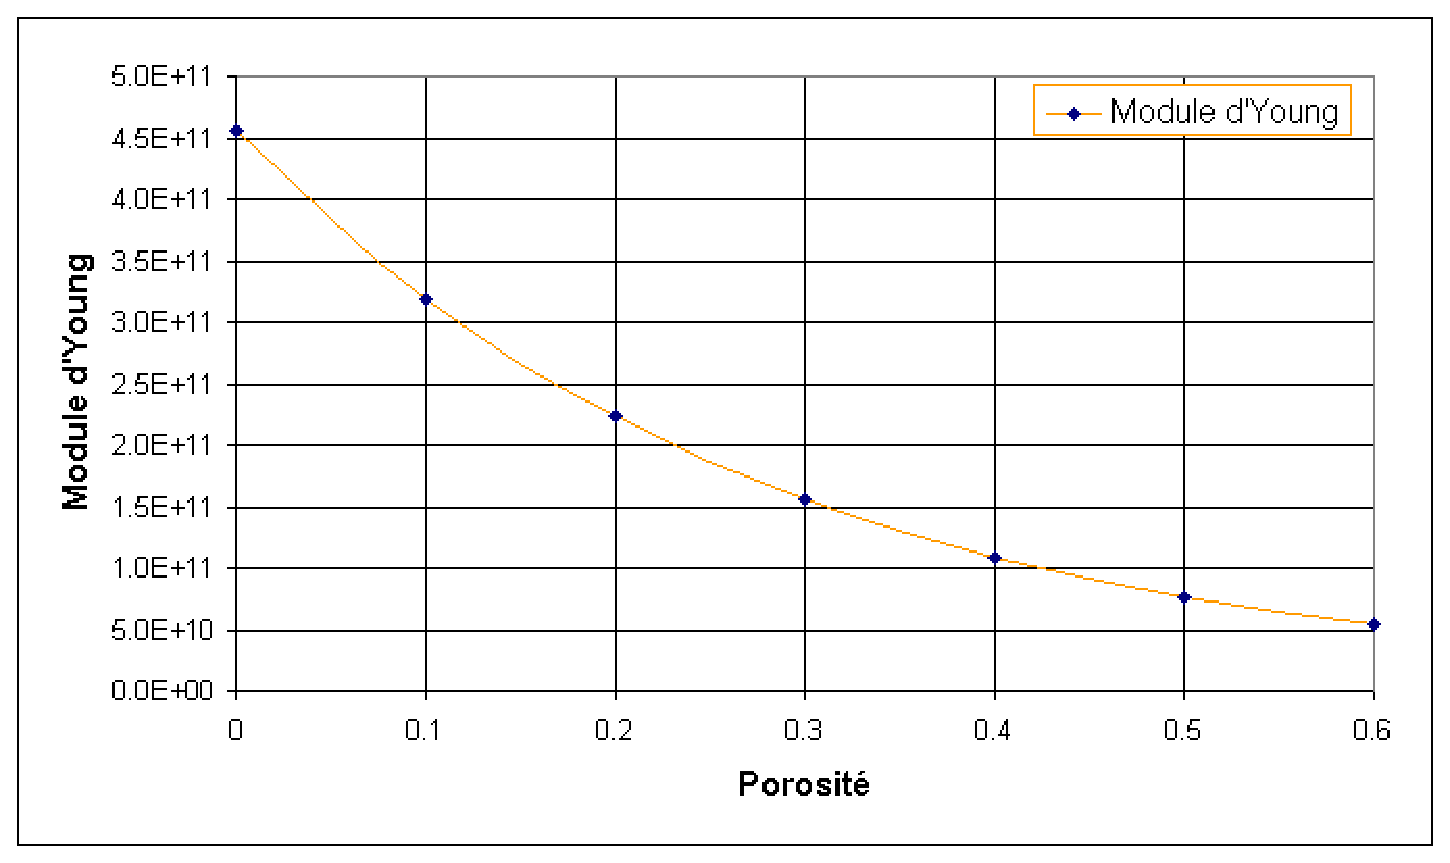
\includegraphics[width=9cm]{Images/mfrontexcel.eps}
  \caption{Graphique \excel{} réalisé à partir d'une
    bibliothèque dynamique généré par \mfront{}.}
  \label{fig:mfrontexcel}
\end{figure}

La figure~\ref{fig:mfrontexcel} montre la dépendance du module
d'\nom{Young} du \sic{} en fonction de la porosité en se basant
sur l'exemple traité au paragraphe~\ref{sec:module-dnomyoung-du}.

\begin{figure}[htbp]
  \centering
  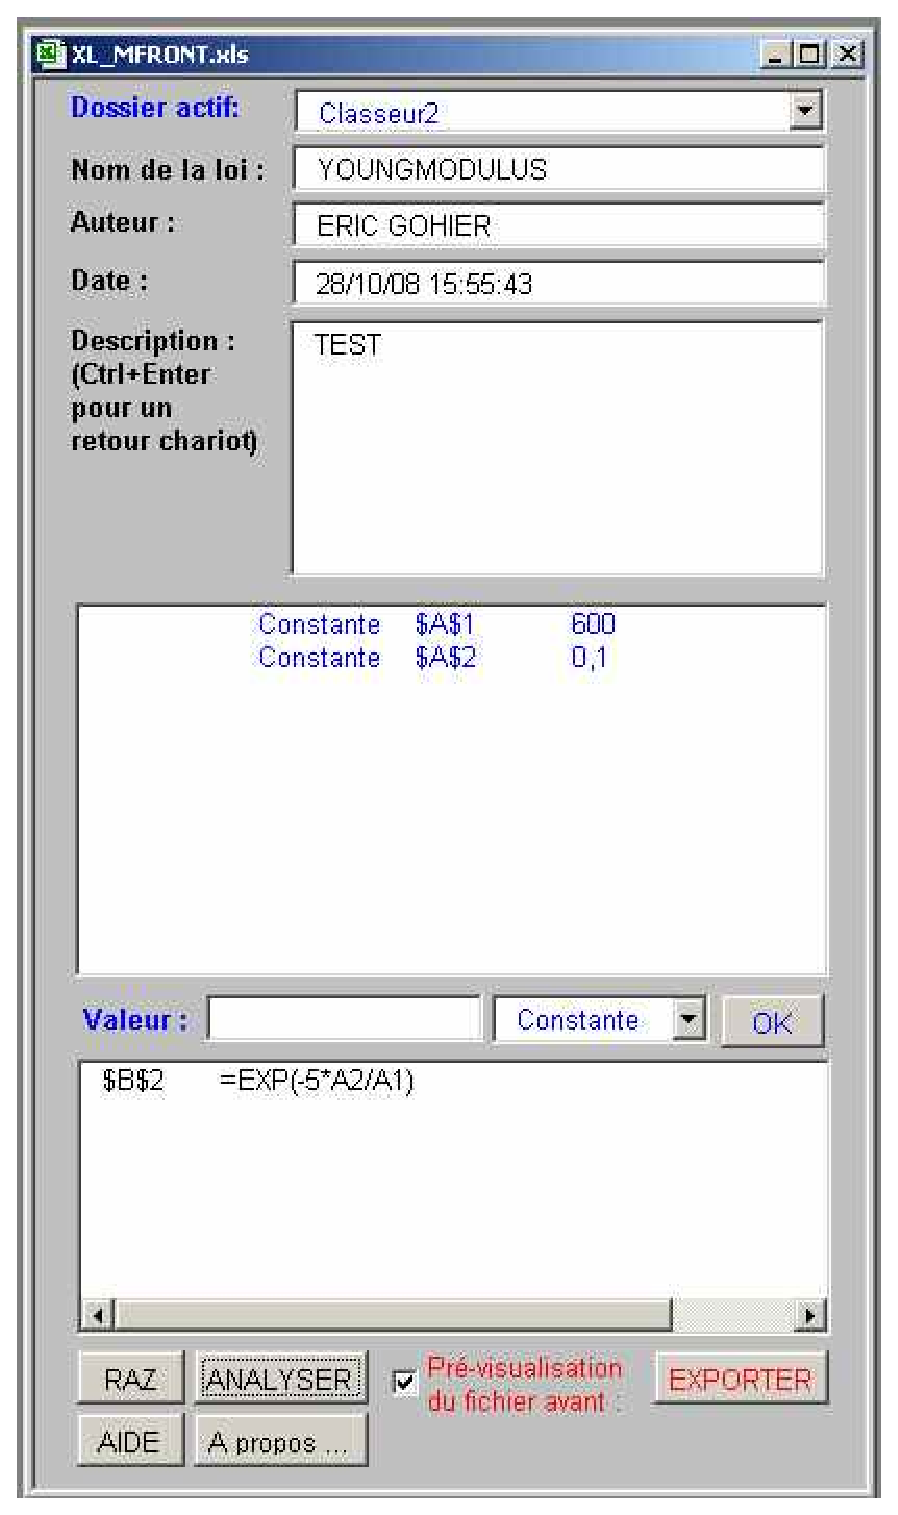
\includegraphics[width=6cm]{Images/mfront.eps}
  \caption{Export d'une formule \excel{} en \mfront{}.}
  \label{fig:exceltomfront}
\end{figure}

\subsection{De \excel{} à \mfront{}} De plus il est apparu utile (et
relativement facile à mettre en \oe{}uvre) de pouvoir directement généré
des fichiers \mfront{} depuis des formules \excel{}. Une macro
\texttt{Visual Basic} a été écrite par \nom{É. Gohier} dans ce but. La
figure~\ref{fig:exceltomfront} montre un exemple de son utilisation.

\begin{figure}[htbp]
  \centering
  \code{
    \noindent
\textcolor{blue}{'DEBPROC'}\hspace*{1em}GETEVOL\hspace*{1em}\hspace*{1em}\hspace*{1em}\hspace*{1em}\hspace*{1em}X0\textcolor{magenta}{*}\textcolor{blue}{'FLOTTANT'}\\
\hspace*{1em}\hspace*{1em}\hspace*{1em}\hspace*{1em}\hspace*{1em}\hspace*{1em}\hspace*{1em}\hspace*{1em}\hspace*{1em}\hspace*{1em}\hspace*{1em}\hspace*{1em}\hspace*{1em}\hspace*{1em}\hspace*{1em}\hspace*{1em}\hspace*{1em}\hspace*{1em}\hspace*{1em}\hspace*{1em}\hspace*{1em}\hspace*{1em}X1\textcolor{magenta}{*}\textcolor{blue}{'FLOTTANT'}\\
\hspace*{1em}\hspace*{1em}\hspace*{1em}\hspace*{1em}\hspace*{1em}\hspace*{1em}\hspace*{1em}\hspace*{1em}\hspace*{1em}\hspace*{1em}\hspace*{1em}\hspace*{1em}\hspace*{1em}\hspace*{1em}\hspace*{1em}\hspace*{1em}\hspace*{1em}\hspace*{1em}\hspace*{1em}\hspace*{1em}\hspace*{1em}\hspace*{1em}nx\textcolor{magenta}{*}\textcolor{blue}{'ENTIER'}\\
\hspace*{1em}\hspace*{1em}\hspace*{1em}\hspace*{1em}\hspace*{1em}\hspace*{1em}\hspace*{1em}\hspace*{1em}\hspace*{1em}\hspace*{1em}\hspace*{1em}\hspace*{1em}\hspace*{1em}\hspace*{1em}\hspace*{1em}\hspace*{1em}\hspace*{1em}\hspace*{1em}\hspace*{1em}\hspace*{1em}TLoi\textcolor{magenta}{*}\textcolor{blue}{'TABLE'}\\
\hspace*{1em}\hspace*{1em}\hspace*{1em}\hspace*{1em}\hspace*{1em}\hspace*{1em}\hspace*{1em}\hspace*{1em}\hspace*{1em}\hspace*{1em}\hspace*{1em}\hspace*{1em}\hspace*{1em}\hspace*{1em}\hspace*{1em}\hspace*{1em}\hspace*{1em}\hspace*{1em}\hspace*{1em}\hspace*{1em}vvar\textcolor{magenta}{*}\textcolor{blue}{'MOT'}\\
\hspace*{1em}\hspace*{1em}\hspace*{1em}\hspace*{1em}\hspace*{1em}\hspace*{1em}\hspace*{1em}\hspace*{1em}\hspace*{1em}\hspace*{1em}\hspace*{1em}\hspace*{1em}\hspace*{1em}\hspace*{1em}\hspace*{1em}\hspace*{1em}\hspace*{1em}\hspace*{1em}values\textcolor{magenta}{*}\textcolor{blue}{'TABLE'};\\
\textcolor{blue}{'MESSAGE'}\hspace*{1em}\textcolor{blue}{'---------------------------------'}\hspace*{1em};\\
\textcolor{blue}{'MESSAGE'}\hspace*{1em}\textcolor{blue}{' Début              : '}\hspace*{1em}X0;\\
\textcolor{blue}{'MESSAGE'}\hspace*{1em}\textcolor{blue}{' Fin                : '}\hspace*{1em}X1;\\
\textcolor{blue}{'MESSAGE'}\hspace*{1em}\textcolor{blue}{' Nombre de valeurs  : '}\hspace*{1em}nx;\\
\textcolor{blue}{'MESSAGE'}\hspace*{1em}\textcolor{blue}{' Loi : librairie    : '}\hspace*{1em}TLoi\textcolor{green}{.}\textcolor{blue}{'LIBRAIRIE'};\\
\textcolor{blue}{'MESSAGE'}\hspace*{1em}\textcolor{blue}{' Loi : Modèle       : '}\hspace*{1em}TLoi\textcolor{green}{.}\textcolor{blue}{'MODELE'};\\
vdime=(\textcolor{blue}{'VALEUR'}\hspace*{1em}\textcolor{blue}{'DIME'});\\
velem=(\textcolor{blue}{'VALEUR'}\hspace*{1em}\textcolor{blue}{'ELEM'});\\
\textcolor{blue}{'OPTION'}\hspace*{1em}\textcolor{blue}{'DIME'}\hspace*{1em}\textcolor{green}{1};\\
\textcolor{blue}{'OPTION'}\hspace*{1em}\textcolor{blue}{'ELEM'}\hspace*{1em}SEG2;\\
lx\hspace*{1em}=\hspace*{1em}\textcolor{blue}{'DROIT'}\hspace*{1em}(\textcolor{blue}{'POIN'}\hspace*{1em}X0)\hspace*{1em}(\textcolor{blue}{'POIN'}\hspace*{1em}X1)\hspace*{1em}nx;\\
modv\hspace*{1em}=\hspace*{1em}\textcolor{blue}{'MODELISER'}\hspace*{1em}lx\hspace*{1em}\textcolor{blue}{'THERMIQUE'}\hspace*{1em}\textcolor{blue}{'ISOTROPE'};\\
xx\hspace*{1em}=\hspace*{1em}\textcolor{blue}{'COORDONNEE'}\hspace*{1em}\textcolor{green}{1}\hspace*{1em}lx\hspace*{1em};\\
vpo\hspace*{1em}=\hspace*{1em}\textcolor{blue}{'CHANGER'}\hspace*{1em}xx\hspace*{1em}\textcolor{blue}{'COMP'}\hspace*{1em}vvar;\\
vel\hspace*{1em}=\hspace*{1em}\textcolor{blue}{'CHANGER'}\hspace*{1em}\textcolor{blue}{'CHAM'}\hspace*{1em}vpo\hspace*{1em}modv\hspace*{1em};\\
nb\hspace*{1em}\hspace*{1em}=\hspace*{1em}\textcolor{blue}{'DIME'}\hspace*{1em}(TLoi\textcolor{green}{.}\textcolor{blue}{'VARIABLES'});\\
\textcolor{blue}{'REPETER'}\hspace*{1em}bcl\hspace*{1em}nb;\\
\hspace*{1em}\hspace*{1em}\hspace*{1em}vvari\hspace*{1em}=\hspace*{1em}\textcolor{blue}{'EXTRAIRE'}\hspace*{1em}(Tloi\textcolor{green}{.}\textcolor{blue}{'VARIABLES'})\hspace*{1em}\&bcl;\\
\hspace*{1em}\hspace*{1em}\hspace*{1em}\textcolor{blue}{'SI'}(\textcolor{blue}{'NEG'}\hspace*{1em}vvari\hspace*{1em}vvar);\\
\hspace*{1em}\hspace*{1em}\hspace*{1em}\hspace*{1em}\hspace*{1em}\hspace*{1em}vel\hspace*{1em}=\hspace*{1em}vel\hspace*{1em}\textcolor{blue}{'ET'}\hspace*{1em}(\textcolor{blue}{'MANUEL'}\hspace*{1em}\textcolor{blue}{'CHML'}\hspace*{1em}modv\hspace*{1em}vvari\hspace*{1em}(values\textcolor{green}{.}vvari));\\
\hspace*{1em}\hspace*{1em}\hspace*{1em}\textcolor{blue}{'FINSI'};\\
\textcolor{blue}{'FIN'}\hspace*{1em}bcl;\\
matE\hspace*{1em}=\hspace*{1em}\textcolor{blue}{'MANUEL'}\hspace*{1em}\textcolor{blue}{'CHML'}\hspace*{1em}modv\hspace*{1em}\textcolor{blue}{'Y'}\hspace*{1em}TLoi;\\
Kel\hspace*{1em}=\hspace*{1em}\textcolor{blue}{'VARI'}\hspace*{1em}\textcolor{blue}{'NUAG'}\hspace*{1em}modv\hspace*{1em}matE\hspace*{1em}vel;\\
Kpo\hspace*{1em}=\hspace*{1em}\textcolor{blue}{'CHANGER'}\hspace*{1em}\textcolor{blue}{'CHPO'}\hspace*{1em}Kel\hspace*{1em}modv\hspace*{1em};\\
evabs\hspace*{1em}=\hspace*{1em}\textcolor{blue}{'EVOL'}\hspace*{1em}\textcolor{blue}{'CHPO'}\hspace*{1em}vpo\hspace*{1em}lx\hspace*{1em}vvar;\\
evordo\hspace*{1em}=\hspace*{1em}\textcolor{blue}{'EVOL'}\hspace*{1em}\textcolor{blue}{'CHPO'}\hspace*{1em}Kpo\hspace*{1em}lx\hspace*{1em}\textcolor{blue}{'Y'};\\
labs\hspace*{1em}=\hspace*{1em}\textcolor{blue}{'EXTRAIRE'}\hspace*{1em}evabs\hspace*{1em}\textcolor{blue}{'ORDO'}\hspace*{1em};\\
lordo\hspace*{1em}=\hspace*{1em}\textcolor{blue}{'EXTRAIRE'}\hspace*{1em}evordo\hspace*{1em}\textcolor{blue}{'ORDO'}\hspace*{1em};\\
cou\hspace*{1em}=\hspace*{1em}\textcolor{blue}{'EVOL'}\hspace*{1em}\textcolor{blue}{'MANUEL'}\hspace*{1em}labs\hspace*{1em}vvar\hspace*{1em}lordo\hspace*{1em};\\
cou\hspace*{1em}=\hspace*{1em}cou\hspace*{1em}\hspace*{1em}\textcolor{blue}{'COULEUR'}\hspace*{1em}\textcolor{blue}{'JAUNE'};\\
\textcolor{blue}{'OPTION'}\hspace*{1em}\textcolor{blue}{'DIME'}\hspace*{1em}vdime;\\
\textcolor{blue}{'OPTION'}\hspace*{1em}\textcolor{blue}{'ELEM'}\hspace*{1em}velem;\\
\textcolor{blue}{'FINPROC'}\hspace*{1em}cou\hspace*{1em};

  }
  \caption[Code de la procédure \texttt{GETEVOL}]{Procédure utilisée
    pour tracer les valeurs d'une fonction en fonction d'une de ces
    variables (les autres étant fixées).}
  \label{fig:getEvol}
\end{figure}

\clearpage
\newpage
\section{Complément sur l'utilisation des propriétés matériau dans \castem{}}

L'usage a cependant montré qu'il était très pratique de pouvoir tracer
les propriétés matériau dans \castem{}, pour vérification. Nous nous
basons sur l'exemple du module d'\nom{Young} du \sic{}, détaillé au
paragraphe~\ref{sec:module-dnomyoung-du} pour illustrer notre propos.

La procédure \texttt{GETEVOL}, reproduite en figure~\ref{fig:getEvol} a
été écrite dans ce but.

\begin{figure}[htbp]
  \centering
  \code{
    \noindent
\textcolor{blue}{'OPTION'}\hspace*{1em}\textcolor{blue}{'DIME'}\hspace*{1em}\textcolor{green}{3};\\
\textcolor{blue}{'OPTION'}\hspace*{1em}\textcolor{blue}{'ELEM'}\hspace*{1em}\textcolor{blue}{'QUA4'};\\
\newline
TLoi\hspace*{1em}=\hspace*{1em}\textcolor{blue}{'TABLE'};\\
TLoi\textcolor{green}{.}\textcolor{blue}{'LIBRAIRIE'}\hspace*{1em}=\hspace*{1em}\textcolor{blue}{'libCastemMaterialLaw.so'};\\
TLoi\textcolor{green}{.}\textcolor{blue}{'MODELE'}\hspace*{1em}\hspace*{1em}\hspace*{1em}\hspace*{1em}=\hspace*{1em}\textcolor{blue}{'SIC\_YOUNGMODULUS\_SNEAD'};\\
TLoi\textcolor{green}{.}\textcolor{blue}{'VARIABLES'}\hspace*{1em}=\hspace*{1em}\textcolor{blue}{'MOTS'}\hspace*{1em}\textcolor{blue}{'T'}\hspace*{1em}\textcolor{blue}{'PORO'};\\
\newline
val\hspace*{1em}=\hspace*{1em}\textcolor{blue}{'TABLE'};\\
val\textcolor{green}{.}\textcolor{blue}{'PORO'}\hspace*{1em}=\hspace*{1em}\textcolor{green}{0.1};\\
\newline
ev\hspace*{1em}=\hspace*{1em}GETEVOL\hspace*{1em}\textcolor{green}{300.}\hspace*{1em}\textcolor{green}{1500.}\hspace*{1em}\textcolor{green}{100}\hspace*{1em}TLoi\hspace*{1em}\textcolor{blue}{'T'}\hspace*{1em}val;\\
\textcolor{blue}{'DESSIN'}\hspace*{1em}ev;

  }
  \caption{Utilisation de la procédure \texttt{GETEVOL}.}
  \label{fig:TestGetEvol}
\end{figure}

Un exemple d'utilisation de cette procédure est donnée en
figure~\ref{fig:TestGetEvol} où est tracé la dépendance du module
d'\nom{Young} du \sic{} en fonction de la température entre \(300\) et
\(1500\) Kelvins pour une porosité de \(0,1\) avec un échantillonnage de
\(100\) valeurs. La tableau \texttt{val} contient ici les valeurs de
toutes les variables autre que celle servant au tracé.

\begin{figure}[htbp]
  \centering
  \includegraphics[width=9cm,angle=90]{mfront/GetEvol.eps}
  \caption{Résultat de la procédure \texttt{GETEVOL}.}
  \label{fig:TestGetEvol2}
\end{figure}

La courbe résultante est représentée en figure~\ref{fig:TestGetEvol2}.

\clearpage
\newpage
\section{La fonction {\tt umat}}
\label{sec:utilisation_umat}

Le prototype de la fonction {\tt umat} a été initialement défini dans le
code ABAQUS. Ce prototype a été repris dans \castem{}. La compatibilité
avec ABAQUS nécessite cependant de déclarer des champs qui ne sont pas
nécessairement utilisés dans \castem{}.

\begin{figure}[htbp]
  \centering
  \begin{tabular}[htbp]{lll}
    & {\tt {\color{purple} SUBROUTINE} {\color{green} UMAT} ( }&{\tt  STRESS, STATEV, DDSDDE, SSE, SPD, SCD,}\\
    {\color{ceabluecurve} \&} &                   & {\tt RPL, DDSDDT, DRPLDE, DRPLDT,}\\
    {\color{ceabluecurve} \&} &                   & {\tt STRAN, DSTRAN, TIME, DTIME,}\\
    {\color{ceabluecurve} \&} &                   & {\tt TEMP, DTEMP, PREDEF, DPRED,}\\
    {\color{ceabluecurve} \&} &                   & {\tt CMNAME, NDI, NSHR, NTENS, NSTATV,}\\
    {\color{ceabluecurve} \&} &                   & {\tt PROPS, NPROPS, COORDS,}\\
    {\color{ceabluecurve} \&} &                   & {\tt DROT, PNEWDT, CELENT, DFGRD0, DFGRD1,}\\
    {\color{ceabluecurve} \&} &                   & {\tt NOEL, NPT, LAYER, KSPT, KSTEP, KINC )}\\
   \end{tabular}
  \caption{Prototype de la fonction {\tt umat}.}
  \label{fig:umat:prototype}
\end{figure}

\begin{longtable}[htpb]{|p{2.cm}|p{4.cm}|p{9cm}|}
  \endfirsthead \hline \multicolumn{3}{|c|}{Suite de la page
    précédente}\\ \hline \endhead \hline \multicolumn{3}{|r|}{{\em Suite
      à la page suivante}}\\ \hline \endfoot \endlastfoot \hline {\tt
    STRESS } & REAL*8(NTENS) & tenseur des contraintes. En entrée, ce
  tableau donne le tenseur des contraintes à $t_{0}$. En sortie, ce
  tableau doit contenir le tenseur des contraintes à $t_{0}+\Delta t$ \\
  {\tt STATEV } & REAL*8(*) & variables internes. En entrée, ce tableau
  contient les variables internes à $t_{0}$. En sortie, il doit contenir
  les variables internes à $t_{0}+\Delta t$ \\
  {\tt DDSDDE } & REAL*8(NTENS,NTENS) & matrice jacobienne du modèle
  (matrice de Hooke tangente) à $t_{0}+\Delta t$. \\
  {\tt SSE } & REAL*8 & énergie de déformation élastique \\
  {\tt SPD } & REAL*8 & dissipation plastique \\
  {\tt SCD } & REAL*8 & dissipation visqueuse. \\
  {\tt RPL } & REAL*8 & puissance calorifique volumique dégagée par le
  travail mécanique, à $t_{0}+\Delta t$ \\
  {\tt DDSDDT } & REAL*8(NTENS) & dérivée du tenseur des contraintes par
  rapport a la température, à $t_{0}+\Delta t$ \\
  {\tt DRPLDE } & REAL*8(NTENS) & dérivées de RPL par rapport aux
  composantes du tenseur des déformations, à $t_{0}+\Delta t$\\ {\tt
    DRPLDT } & REAL*8 & derivée de RPL par rapport a la température, à
  $t_{0}+\Delta t$. \\
  {\tt STRAN } & REAL*8(NTENS) & tenseur des déformations totales à
  $t_{0}$ \\
  {\tt DSTRAN } & REAL*8(NTENS) & tenseur des incréments de déformation
  totale par rapport a l'état de reference à $t_{0}$ \\
  {\tt TIME } & REAL*8(2) & TIME(1) = 0, TIME(2) = $t_{0}$ où $t_{0}$
  est le précédent instant d'équilibre atteint \\
  {\tt DTIME } & REAL*8 & DTIME = $\Delta t$ où $\Delta t$ est le
  nouveau pas de temps propose par {\tt PASAPAS} pour atteindre
  l'equilibre avec l'incrément de déformation totale impose ({\tt
    DSTRAN}) \\
  {\tt TEMP } & REAL*8 & température à $t_{0}$ \\
  {\tt DTEMP } & REAL*8 & incrément de température à $t_{0}+\Delta t$ \\
  {\tt PREDEF } & REAL*8(*) & vecteur des paramètres externes de la loi
  de comportement, valeurs à $t_{0}$ \\
  {\tt DPRED } & REAL*8(*) & incréments des paramètres externes à
  $t_{0}+\Delta t$ \\
  {\tt CMNAME } & CHARACTER*16 & identifiant de la loi de comportement.
  On conserve le type 'chaine de caracteres' pour l'identifiant de la
  loi, afin de préserver la compatibilité avec ABAQUS. Dans le cas d'une
  adhérence à \castem{}, la loi est identifiée par le numéro qui lui a
  été attribué par l'argument 'NUME\_LOI' de l'opérateur MODE. Par
  convention, ce numéro est encodé dans les 4 derniers caractères de la
  chaîne, et doit être récupéré dans {\tt umat} par une instruction du
  type K4ILOI = CMNAME(13 : 16) où K4ILOI est une variable locale de
  type {\tt CHARACTER*4} \\
  {\tt NDI } & INTEGER & nombre de composantes diagonales du tenseur des
  contraintes \\
  {\tt NSHR } & INTEGER & nombre de composantes extradiagonales du
  tenseur des contraintes. \\
  {\tt NTENS } & INTEGER & nombre de composantes du tenseur des
  contraintes\\ {\tt NSTATV } & INTEGER & nombre de variables internes
  \\
  {\tt PROPS } & REAL*8(NPROPS) & vecteur des propriétés du matériau. \\
  {\tt NPROPS } & INTEGER & nombre de propriétés du matériau \\
  {\tt COORDS } & REAL*8(3) & coordonnees cartésiennes du point
  d'intégration courant \\
  {\tt DROT } & REAL*8(3,3) & matrice d'incréments de rotation. Cette
  matrice décrit la rotation sur le pas de temps de la base dans
  laquelle sont exprimés les tenseurs de contraintes et de déformations.
  \\
  {\tt PNEWDT } & REAL*8 & rapport entre le nouveau pas de temps suggéré
  et le pas de temps donné en entrée \\
  {\tt CELENT } & REAL*8 & longueur caractéristique de l'élément. Dans
  le cas d'une adhérence à \castem{}, cette longueur caractéristique est
  déterminée par {\tt LOCARA} comme la distance maximale entre deux
  noeuds de l'élément. \\
  {\tt DFGRD0 } & REAL*8(3,3) & tenseur gradient de déplacement à
  $t_{0}$ \\
  {\tt DFGRD1 } & REAL*8(3,3) & tenseur gradient de déplacement à
  $t_{0}+\Delta t$ \\
  {\tt NOEL } & INTEGER & numéro de l'élément courant \\
  {\tt NPT } & INTEGER & numéro du point d'intégration courant \\
  {\tt LAYER } & INTEGER & numéro de couche pour des coques composites
  ou des solides multi-couches \\
  {\tt KSPT } & INTEGER & numéro de section dans la couche courante. \\
  {\tt KSTEP } & INTEGER & Cette entrée n'a pas de sens dans le cas
  d'une adhérence à \castem{} \\
  {\tt KINC } & INTEGER & Code de sortie \\
  \hline
  \caption{Arguments de la fonction {\texttt umat}}
  \label{tab:umat:argument}
\end{longtable}

\clearpage
\newpage
\section{Amélioration de la robustesse des algorithmes de résolutions
  implicites}

Les méthodes de résolution des systèmes implicites nécessitent de
choisir une estimation de la solution \(\vec{X}_{0}\) pour initier la
recherche. Par défaut, \mfront{} utilisera le vecteur nul comme
estimation initiale, mais l'utilisateur peut en spécifier une autre par
la directive \mkey{Predictor}.

La convergence des algorithmes de résolutions implicites n'est garantie
que si l'estimation initiale \(\vec{X}_{0}\) est suffisamment proche de
la solution recherchée. Loin de la solution, l'algorithme peut
éventuellement converger mais les premières itérations tendent
généralement vers la solution assez lentement (phase de recherche)~: il
est classique d'observer une convergence linéaire lors de la phase de
recherche et une transition vers un ordre de convergence plus élevé
proche de la solution.

Pour les lois de comportement fortement non linéaires, il est difficile
de proposer une estimation \(\vec{X}_{0}\) garantissant la convergence,
il peut donc être intéressant d'améliorer la robustesse des algorithmes.

\begin{table}
  \centering
  \begin{tabular}{|c|c|}
    \hline
    Méthode & Expression de \(\vec{s}_{n}\) \\
    \hline
    \hline
    Algorithme de \textsc{Newton-Raphson}
    & \(-J^{-1}\,.\,\vec{F}\paren{\vec{X}_{n-1}}\) \\
    \hline
    \begin{minipage}{7cm}
      Algorithme de \textsc{Newton-Raphson} et dérivation numérique
    \end{minipage} &
    \(-\underset{\sim}{J}^{-1}\,.\,\vec{F}\paren{\vec{X}_{n-1}}\) \\
    \hline
    Premier algorithme de \textsc{Broyden} &
    \begin{minipage}{5cm}
      \(-\underset{\sim}{J}_{n-1}^{-1}\,.\,\vec{F}\paren{\vec{X}_{n-1}}\)
      où \(\underset{\sim}{J}_{n}\) est donné par
      l'équation~\eqref{eq:Broyden}
    \end{minipage} \\
    \hline
    Second algorithme de \textsc{Broyden} &
    \begin{minipage}{5cm}
      \(-\underset{\sim}{J}_{n-1}^{-1}\,.\,\vec{F}\paren{\vec{X}_{n-1}}\)
      où \(\underset{\sim}{J}_{n}^{-1}\) est donné par\(\vec{X}_{0}\)
      l'équation~\eqref{eq:Broyden2}
    \end{minipage} \\
    \hline
  \end{tabular}
  \label{tab:sn}
\end{table}

L'ensemble des algorithmes présentés jusqu'ici prennent la forme~:
\[
\vec{X}_{n}=\vec{X}_{n-1}+\vec{s}^{N}_{n}
\]
L'expression du pas \(s^{N}_{n}\) pour les différentes algorithmes
présentés est donnée au tableau~\ref{tab:sn}. D'après la discussion
précédente, ce pas \(s^{N}_{n}\) est optimal proche de la solution
finale.

Il est intéressant de trouver une autre estimation de la solution, moins
performante près de la solution mais plus robuste. Les méthodes
précédentes donnant une approximation du jacobien, il peut être
intéressant de substituer à la fonction \(F\) son application tangente
et de choisir cette nouvelle estimation comme la solution du problème de
minimisation suivant~:
\[
\min_{\vec{s}^{G}\,\in\,\mathcal{R}^{N}}\,\norm{\vec{F}\paren{\vec{X}_{n-1}}+J\paren{\vec{X}_{n-1}}\,.\,\vec{s}^{G}}
\]

La solution de ce problème est donnée par\footnote{Pour le prouver,
  nous pouvons écrire que~:
  \[
  \begin{array}{rcl}
    \norm{\vec{F}\paren{\vec{X}_{n-1}}+J\paren{\vec{X}_{n-1}}\,.\,\vec{s}^{G}}^{2}
    &=& {F}\paren{\vec{X}_{n-1}}\,.\,{F}\paren{\vec{X}_{n-1}}+2\,\vec{F}\paren{\vec{X}_{n-1}}\,\mid\,J\paren{\vec{X}_{n-1}}\,.\,\vec{s}^{G} \\
    &&+\paren{J\paren{\vec{X}_{n-1}}\,.\,\vec{s}^{G}}\,\mid\,\paren{J\paren{\vec{X}_{n-1}}\,.\,\vec{s}^{G}}
  \end{array}
  \]
  Le gradient de cette expression est égal à~:
  \[
  2\,\mbox{}^{t}J\paren{\vec{X}_{n-1}}\vec{F}\paren{\vec{X}_{n-1}}+\mbox{}^{t}J\paren{\vec{X}_{n-1}}\,J\paren{\vec{X}_{n-1}}\,.\vec{s}^{G}
  \]
}~:
\[
\mbox{}^{t}J\paren{\vec{X}_{n-1}}\,J\paren{\vec{X}_{n-1}}\,.\vec{s}^{G}=-\,\mbox{}^{t}J\paren{\vec{X}_{n-1}}\,.\,\vec{F}\paren{\vec{X}_{n-1}}
\]
Ce pas est intéressant loin de la solution.

Les pas \(\vec{s}^{N}_{n}\) et \(\vec{s}_{n}^{G}\) sont combinés ainsi~:
\[
\vec{s} = a_{n} \,\vec{s}^{G}_{n} + \paren{1-a_{n}}\,\vec{s}_{n}^{N}
\]

\clearpage
\newpage
\section{Description de l'algorithme \nom{Runge-Kutta}-\castem{}}
\label{sec:algo}
% $Y$ représente les vecteurs de variables internes et 

G représente une fonction a priori non linéaire et que nous supposerons
a minima continûment dérivable. On cherche à résoudre le système
différentiel suivant:
\begin{equation}
  \label{eq:systeme_diff:RK}
  \dot{Y}=G\paren{Y,t}
\end{equation}

La résolution numérique de cette équation consiste à estimer, à partir
de la valeur \(\debutpas{Y}\) à un instant \(t\), la valeur
\(\finpas{Y}\) à un instant \(t+\Delta\, t\).

Voici une description de l'algorithme \nom{Runge-Kutta}-\castem{}~:
\begin{itemize}
\item première estimation d'une solution à \(\Delta\, t /2\)~:
\begin{subequations}
\begin{align}
  \dot{Y}_1 &= G\paren{\debutpas{Y},t} \\
  \demipas{Y_1} &= \debutpas{Y} + \Frac{\Delta\, t}{2} \dot{Y}_1
\end{align}
\end{subequations}
\item deuxième estimation d'une solution à \(\Delta\, t /2\)~:
\begin{subequations}
\begin{align}
  \dot{Y}_2 &= G\paren{Y_1,t} \\
  \demipas{Y_{12}} &= \debutpas{Y} + \Frac{\Delta\, t}{2} \paren{\Frac{\dot{Y}_1 + \dot{Y}_2}{2}}
\end{align}
\end{subequations}
\item première estimation d'une solution à \(\Delta\, t\)~:
\begin{subequations}
\begin{align}
  \dot{Y}_3 &= G\paren{Y_{12},t} \\
  \finpas{Y_{13}} &= \demipas{Y_{12}} + \Frac{\Delta\, t}{2} \dot{Y}_3
\end{align}
\end{subequations}
\item deuxième estimation d'une solution à \(\Delta\, t\)~:
\begin{subequations}
\begin{align}
  \dot{Y}_4 &= G\paren{Y_{13},t} \\
\label{eq:estimation_yf}
\finpas{Y_f} &= \demipas{Y_{12}} + \Frac{\Delta\,
  t}{2} \paren{\Frac{\dot{Y}_3 + \dot{Y}_4}{2}}
\end{align}
\end{subequations}
\item troisième estimation d'une solution à \(\Delta\, t\)~:
\begin{subequations}
\begin{align}
  \dot{Y}_5 &= G\paren{Y_f,t} \\
\label{eq:estimation_y5}
\finpas{Y_5} &= \debutpas{Y} + \Delta\, t \paren{\Frac{\dot{Y}_1 +
    4\dot{Y}_3 + \dot{Y}_5}{6}}
\end{align}
\end{subequations}
\end{itemize}

Dans le cas où le calcul d'une de ces estimations ne pourraient être
calculés, un sous-découpage du pas de temps est effectué comme le montre
l'algorithme décrivant le sous-découpage du pas temps (\textsc{Fig.}
\ref{fig:algo_temps}).

Une fois toutes ces estimations calculées, on compare les contraintes
obtenues lors des estimations \(\finpas{Y_f}\) (\ref{eq:estimation_yf})
et \(\finpas{Y_5}\) (\ref{eq:estimation_y5}), notées respectivement
\(\finpas{\tsigma}\) et \(\tsigma_5\).

Pour cela, on se donne une erreur dont l'amplitude est basée sur la
valeur des contraintes en début de pas \(\debutpas{\tsigma}\) ou sur la
valeur du module d'\nom{Young} \(E\)~:
\[
errabs = \left\{
\begin{aligned}
  \sqrt{\debutpas{\tsigma}:\debutpas{\tsigma}}\,\times\,10^{-5} &\textrm{ si }\sqrt{\debutpas{\tsigma}:\debutpas{\tsigma}}>E\,\times\,10^{-3} \\
  E\,\times\,10^{-8}                       &\textrm{ si }\sqrt{\debutpas{\tsigma}:\debutpas{\tsigma}}<E\,\times\,10^{-3}
\end{aligned}
\right.
\]

On définit deux variables représentant
l'écart des contraintes \(ra\) et \(sqra\) définies de la manière
suivante :
\begin{align}
  ra &=
  \Frac{\sqrt{\paren{\finpas{\tsigma}-\tsigma_5}:\paren{\finpas{\tsigma}-\tsigma_5}}}{errabs}\\
  sqra &= \sqrt{ra}\\
\end{align}

En testant ces deux paramètres avec des critères (fixés), on établit la
convergence ou la non-convergence du calcul ainsi que le nouvel
incrément de temps \(\Delta\, t\) qui sera utilisé. Dans le code de
calcul, cet incrément de temps \(\Delta\, t\) est noté \texttt{dt\_}.
L'algorithme déterminant le nouvel incrément de temps est présenté à la
figure~\ref{fig:algo_temps}. Dans cet algorithme, le temps est initial
est noté \texttt{t} tandis que le temps final est noté \texttt{dt}. La
variable \texttt{dtprec} est définie comme une valeur minimale du
sous-découpage \texttt{dt\_} en deçà de laquelle on renvoie une erreur.

\begin{figure}[htbp]
\centering
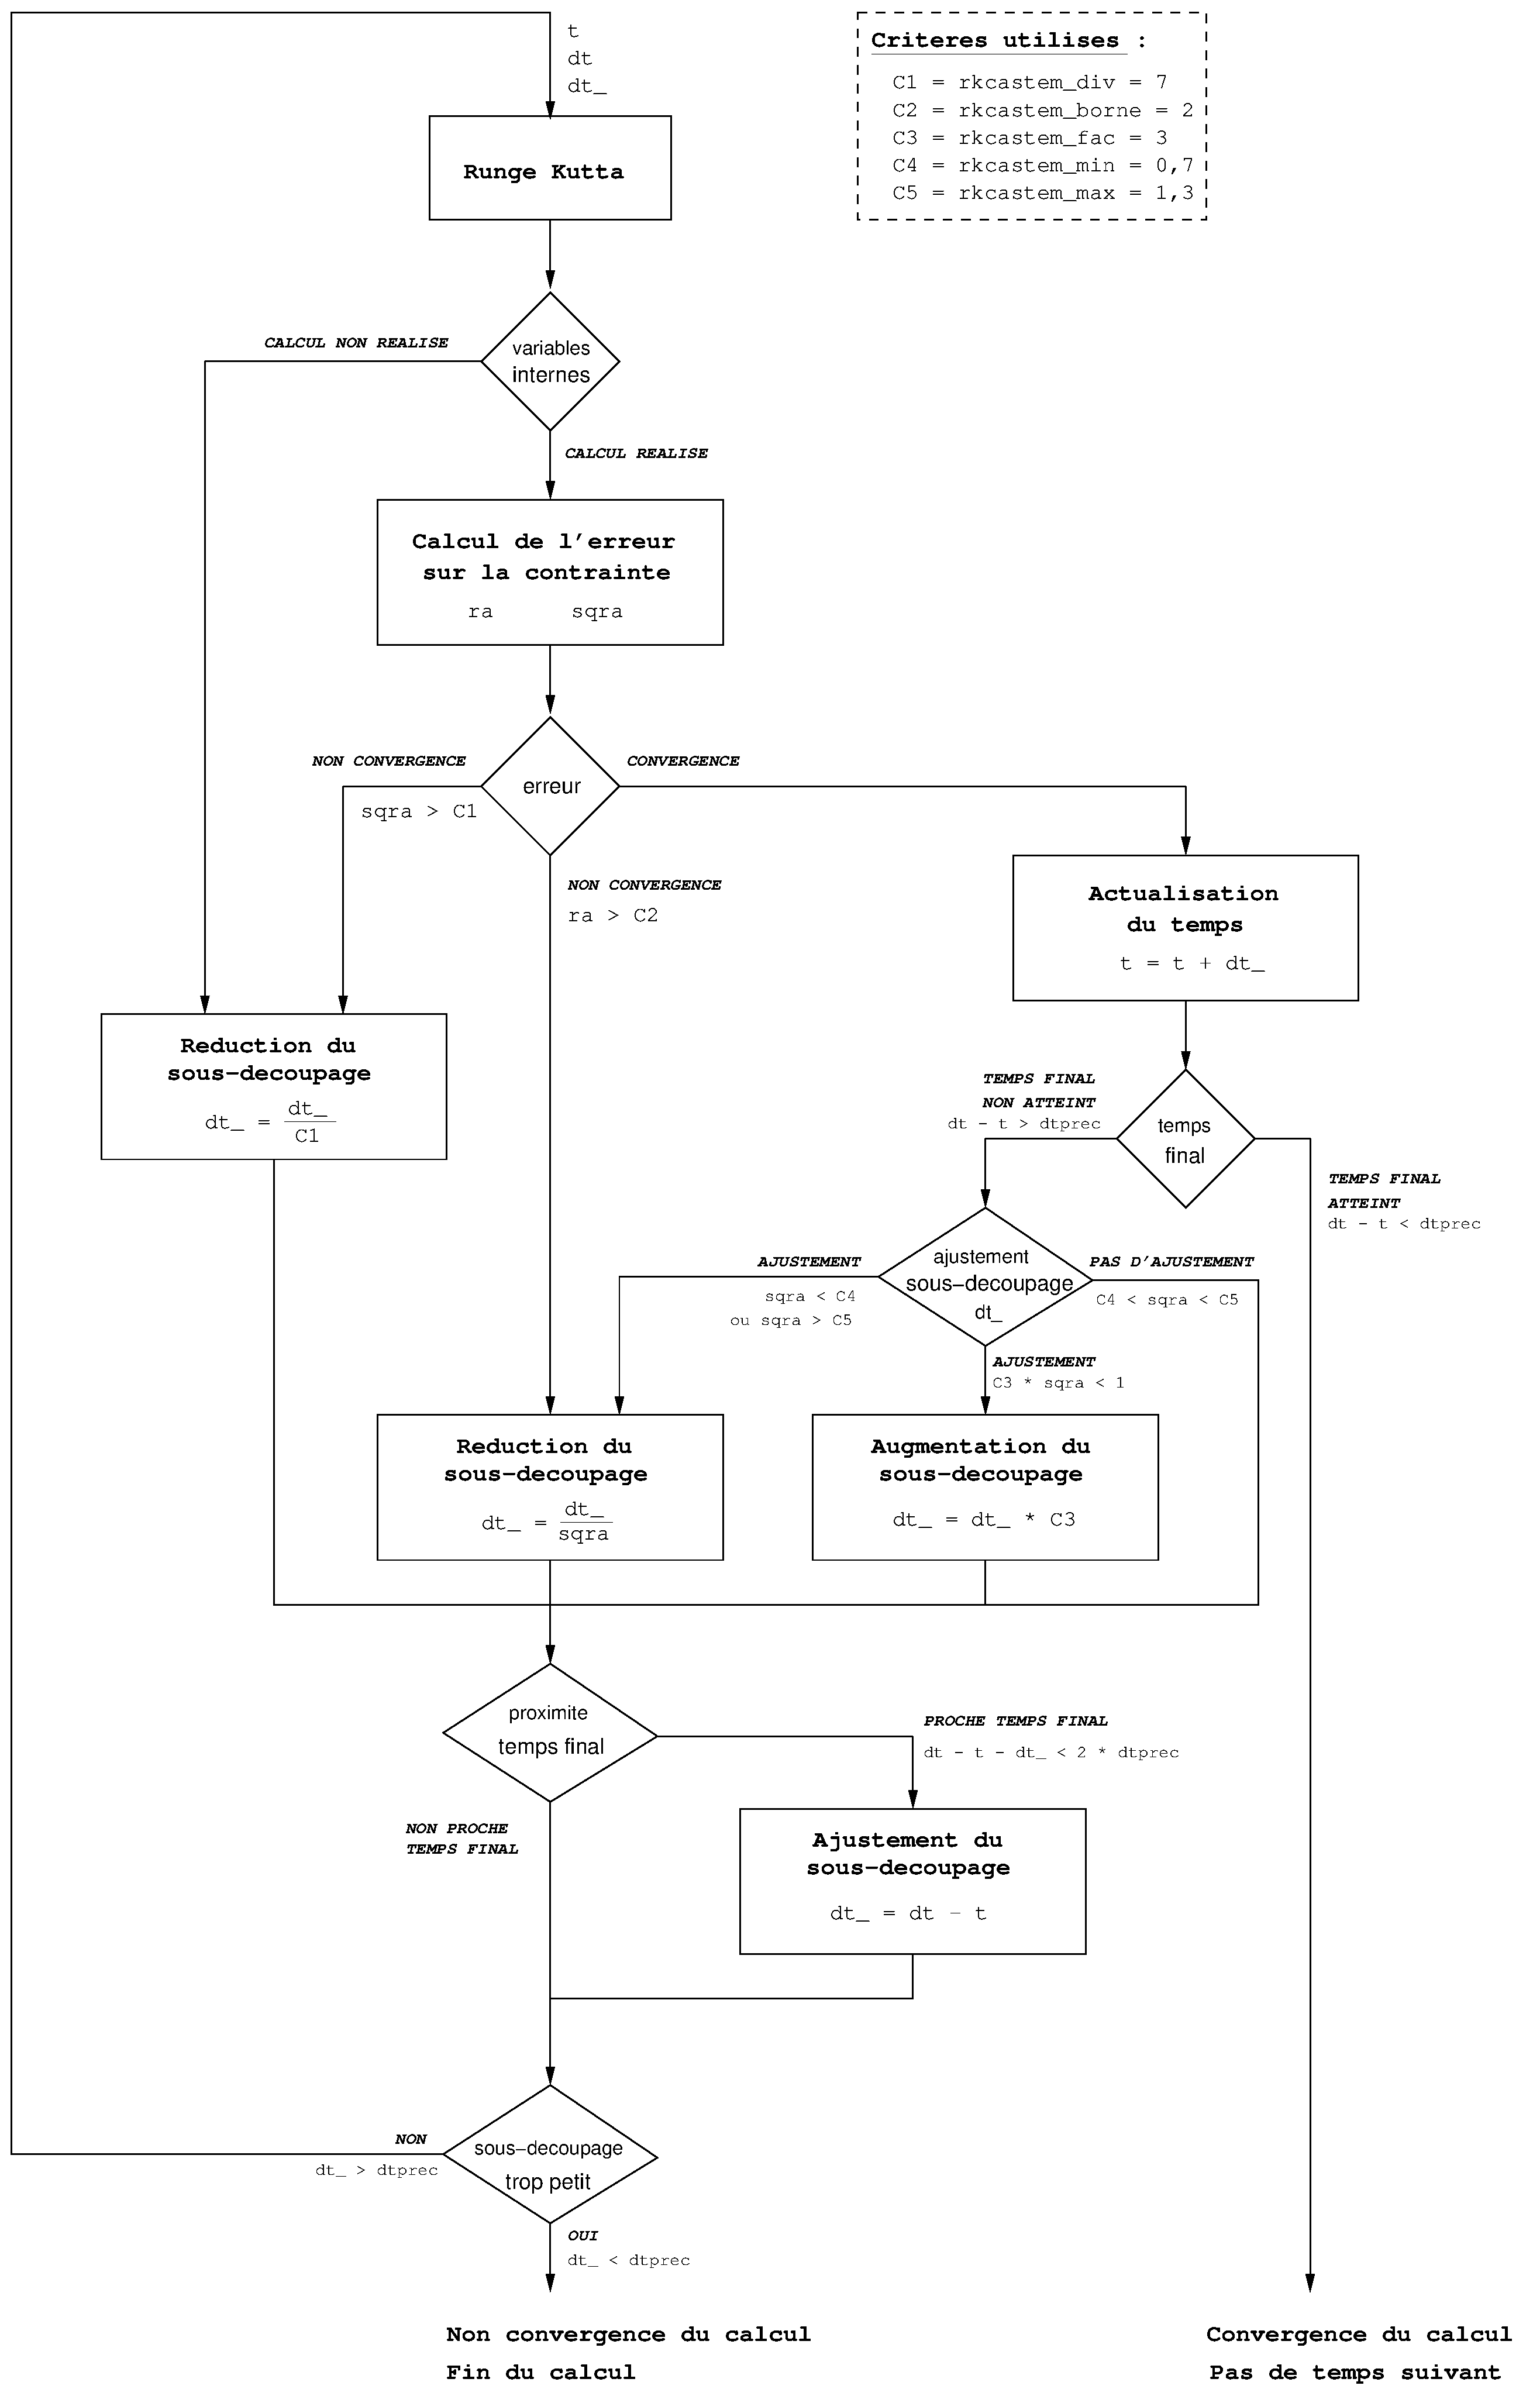
\includegraphics[width=0.9\textwidth,height=22cm]{Images/Algo_temps.eps}
\caption{Description de l'algorithme pour déterminer le sous-découpage du pas de temps}
\label{fig:algo_temps}
\end{figure}

\clearpage
\newpage
%%%%%%%%%%%%%%%%%%%%%%%%%%%%%%%%%%%%%%%%%%%
% File      : annexe-orthotropie
% Author    : THOMAS HELFER
% Date      : 7 mer. 2012
% Directory : /home/th202608/codes/MFrontMaterials/trunk/src/trunk/docs/description
%%%%%%%%%%%%%%%%%%%%%%%%%%%%%%%%%%%%%%%%%%%

\section{Rappels sur les lois de comportement orthotropes et application
  aux tubes}
\label{sec:annexe:orthotropie}

Un matériau (mécaniquement) orthotrope possède, en chaque point
d'espace, trois plans de symétrie ortho\-gonaux vis à vis de son
comportement mécanique. Ces trois plans définissent trois directions
perpendiculaires appelées directions d'ortho\-tropie.

Un repère d'orthotropie est un repère orthonormé formé par ces trois
directions. Le problème traité amène souvent à privilégier un de ces
repères pour décrire le comportement mécanique du matériau. Le cas des
tubes sera par exemple traité en détails au
paragraphe~\ref{sec:conv-de-rang}. Le repère est alors appelé le repère
d'orthotropie du matériau. Les trois directions associées à ce repère
sont simplement notées \(1\), \(2\) et \(3\). {\em Dans la suite,
  l'expression de la loi de comportement mécanique, de la matrice de
  souplesse et des différents tenseurs, se fera toujours dans ce
  repère.}

\subsection{Directions d'orthotropie}
\label{sec:orthotropie}

Le tenseur des  contraintes sera dans la suite représenté sous forme
vectorielle. En \(3D\), ce tenseur s'écrira donc~:
\begin{equation}
  \label{eq:tsigma}
  \tsigma = \left(
    \begin{array}{c}
      \sigma_{11} \\
      \sigma_{22}  \\
      \sigma_{33}  \\
      \sqrt{2}\,\sigma_{12} \\
      \sqrt{2}\,\sigma_{13} \\
      \sqrt{2}\,\sigma_{23} \\
    \end{array}
  \right)
\end{equation}

De même, le tenseur des déformations totales sera représenté par le
vecteur suivant~:
\begin{equation}
  \label{eq:tepsilonto}
  \tepsilonto = \left(
    \begin{array}{c}
      \epsilonto_{11} \\
      \epsilonto_{22}  \\
      \epsilonto_{33}  \\
      \sqrt{2}\,\epsilonto_{12} \\
      \sqrt{2}\,\epsilonto_{13} \\
      \sqrt{2}\,\epsilonto_{23} \\
    \end{array}
  \right)
\end{equation}

Contrairement aux notations de \nom{Voigt} utilisées par le code aux
éléments finis \castem{}, ces notations permettent de symétriser le
rôle des contraintes et des déformations et de substituer au produit
doublement contracté de deux tenseurs le produit scalaire de leurs
représentations vectorielles. Cette symétrie des tenseurs des
contraintes et de déformations est particulièrement utile quand des
calculs tensoriels complexes sont nécessaires.

Notons que l'ordre des composantes de cisaillement n'est pas celui des
notations de \nom{Voigt}, mais reprend celui utilisé par le code aux
éléments finis \castem{}.

\subsection{Élasticité}
\label{sec:elasticite}

Dans le cadre de l'élasticité linéaire, les contraintes $\tsigma$ sont
liées aux déformations élastiques $\tepsilonel$ par la {\bf matrice de
  rigidité}, appelée également {\bf matrice d'élasticité} dans la
suite et notée $\tenseurq{D}$, ou par son inverse, la {\bf matrice de
  souplesse}, notée $\tenseurq{S}$, par la relation~:
\[
\tsigma=\tenseurq{D}:\tepsilonel
,\quad\text{et}\quad
\tepsilonel=\tenseurq{S}:\tsigma
.\]

La matrice de souplesse d'un matériau orthotrope s'écrit, dans le
repère d'orthotropie, sous la forme~:
\begin{equation}
  \label{eq:S}
  \tenseurq{S}=
  \begin{pmatrix}
    \Frac{1}{E_1}&-\Frac{\nu_{12}}{E_1}&-\Frac{\nu_{13}}{E_1}&0&0&0\\
    -\Frac{\nu_{21}}{E_2}&\Frac{1}{E_2}&-\Frac{\nu_{23}}{E_2}&0&0&0\\
    -\Frac{\nu_{31}}{E_3}&-\Frac{\nu_{32}}{E_3}&\Frac{1}{E_3}&0&0&0\\
    0&0&0&\Frac{1}{2\,G_{12}}&0&0\\
    0&0&0&0&\Frac{1}{2\,G_{13}}&0\\
    0&0&0&0&0&\Frac{1}{2\,G_{23}}\\
  \end{pmatrix}
\end{equation}
Elle est donc caractérisée par \(9\) coefficients indépendants~:
\begin{itemize}
\item \(3\) modules d'\nom{Young} $E_1$, $E_2$ et $E_3$~;
\item \(3\) coefficients de \nom{Poisson} $\nu_{12}$, $\nu_{13}$ et
  $\nu_{23}$~;
\item \(3\) modules de cisaillement $G_{12}$, $G_{13}$ et $G_{23}$.
\end{itemize}

Le facteur \(2\) apparaissant sur les modules de cisaillement est dû à
la convention de représentation des tenseurs utilisée dans cette note
(paragraphe~\ref{sec:orthotropie}) et est introduit pour que la
définition des modules d'élasticité soit cohérente avec les conventions
\castem{} qui utilise une notation proche de celle de \nom{Voigt}. En
particulier, les termes de cisaillement s'écrivent~:
\[
\sigma_{12} = 2\,G_{12}\epsilonel_{12}
\]

Les trois coefficients de Poisson, $\nu_{21}$, $\nu_{31}$ et
$\nu_{32}$ vérifient les relations imposées par la symétrie de la
matrice $\tenseurq{S}$~:
\[
\nu_{21}=\Frac{E_2}{E_1}\,\nu_{12}
,\quad
\nu_{31}=\Frac{E_3}{E_1}\,\nu_{13}
\quad\text{et}\quad
\nu_{32}=\Frac{E_3}{E_2}\,\nu_{23}
,\]

\subsection{Critère de \nom{Hill}}
\label{sec:critere-de-nomhill}

Par analogie avec l'usage courant pour les matériaux isotropes et en
accord avec l'expérience, la plupart des écoulements plastiques ou
viscoplastiques sont décrits en introduisant une variable scalaire de
l'état des contraintes, la contrainte équivalente de \nom{Hill}, notée
dans la suite \(\sigmaH\)~\cite{cha_1996,caill_98}. L'intensité de
l'écoulement est fonction de cette contrainte équivalente et les
composantes du tenseur des contraintes n'interviennent pas
explicitement.

Bien que cela ne soit pas nécessaire, nous ferons dans la suite
l'hypothèse de normalité de l'écoulement~: la direction d'écoulement
est donnée par la normale aux iso-surfaces de la contrainte
équivalente.

\paragraph{Tenseur de Hill}

Avant de donner l'expression de la contrainte équivalente, il est
pratique d'introduire un tenseur d'ordre \(4\), nommé dans la suite
tenseur de \nom{Hill} et noté \tenseurq{H}~:
\begin{equation}
  \label{eq:H}
  \tenseurq{H} =
  \left(
    \begin{array}{cccccc}
      F+H & -F  & -H  & 0 & 0 & 0 \\
      -F  & G+F & -G  & 0 & 0 & 0 \\
      -H  & -G  & H+G & 0 & 0 & 0 \\
      0   & 0   & 0   & L & 0 & 0 \\
      0   & 0   & 0   & 0 & M & 0 \\
      0   & 0   & 0   & 0 & 0 & N \\
    \end{array}
  \right)
\end{equation}
où les \(6\) coefficients \(F\), \(G\), \(H\), \(L\), \(M\) et \(N\)
doivent être identifiés expérimentalement.

\paragraph{Contrainte équivalente au sens de \nom{Hill}}

La contrainte équivalente au sens de \nom{Hill} s'écrit
classiquement~:
\[
\sigmaH = \sqrt{\tsigma\colon\,\tenseurq{H}\colon\, \tsigma}
\]

En développant cette expression avec les conventions d'écriture du
tenseur des contraintes décrites par l'équation~\eqref{eq:tsigma},
nous obtenons~:
\begin{equation}
  \label{eq:sigH}
  \sigmaH = \sqrt{\left(\sigma_{22}-\sigma_{11}\right)^2\,F +
    \left(\sigma_{33}-\sigma_{22}\right)^2\,G +
    \left(\sigma_{11}-\sigma_{33}\right)^2\,H +
    2\,\sigma_{12}^2\,L +
    2\,\sigma_{13}^2\,M +
    2\,\sigma_{23}^2\,N}
\end{equation}

\paragraph{Tenseur normal} Le tenseur normal \(\tenseur{n}\) est
défini comme la normale aux iso-surfaces de la contrainte équivalente.
Il est donc égal à~:
\begin{equation}
  \label{eq:n}
  \tenseur{n} = \deriv{\sigmaH}{\tsigma} = \Frac{1}{2\,\sqrt{\tsigma\colon\,\tenseurq{H}\colon\, \tsigma}}\,\deriv{}{\tsigma}\paren{\tsigma\colon\,\tenseurq{H}\colon\, \tsigma} = \Frac{1}{\sigmaH}\,\tenseurq{H}\colon\, \tsigma
\end{equation}

\paragraph{Incompressibilité} Il est aisé de vérifier que le tenseur
\(\tenseurq{H}\colon\, \tsigma\), et donc le tenseur normal
\(\tenseur{n}\) sont déviatoriques (de trace nulle).  L'écoulement
associé est donc {\em incompressible}.

\paragraph{Lien avec l'isotropie} Les lois d'écoulement isotropes
dépendent généralement de la contrainte équivalente de \nom{Von
  Mises} qui est donnée par la relation~:
\[
\sigmaeq = \sqrt{\tsigma\colon\,\tenseurq{M}\colon\, \tsigma}
\]
où \(\tenseurq{M}\) est le tenseur d'ordre \(4\) égal à
\(\Frac{3}{2}\paren{\tenseurq{I}-\Frac{1}{3}\tenseur{I}\otimes\tenseur{I}}\).
Le tenseur \(\tenseurq{I}-\Frac{1}{3}\tenseur{I}\otimes\tenseur{I}\),
généralement noté \(\tenseurq{K}\), projette un tenseur d'ordre \(2\)
sur l'espace des tenseurs déviatoriques (de trace nulle).

Le tenseur \(\tenseurq{M}\) est un cas particulier du tenseur
\(\tenseurq{H}\) obtenu pour les coefficients~:
\[
\left\{
  \begin{aligned}
    F &= G &= H &= \Frac{1}{2} \\
    L &= M &= N &= \Frac{3}{2}
  \end{aligned}
\right.
\]

Les termes \(L\), \(M\) et \(N\) sont difficiles à évaluer
expérimentalement (et inaccessibles dans des essais sur tube chargé en
pression interne). Ils sont souvent supposés égaux à la valeur qu'ils
auraient pour un matériau isotrope.

\subsection{Conventions de rangement des directions d'orthotropie pour
  les tubes en fonction de l'hypothèse de modélisation}
\label{sec:conv-de-rang}

L'écriture des lois de comportements mécaniques sous forme tensorielle
garantie théoriquement que l'écriture de la loi est indépendante de
l'hypothèse de modélisation utilisée (\(1D\), \(2D\paren{r,\theta}\),
\(2D\paren{r,z}\) ou \(3D\)). Les restrictions imposées par le code aux
éléments finis \castem{} sur la définition des directions d'orthotropie
rendent cependant impossible une telle écriture. Ce paragraphe traite
cette question en détails dans le cas des tubes et explicite les choix
faits pour l'écriture des lois de comportements orthotropes.

Le code aux éléments finis \castem{} ne permettant pas à l'utilisateur
de modifier le rangement des axes en \(1D\), cette hypothèse de
modélisation impose que~:
\begin{itemize}
\item le premier axe d'orthotropie soit la direction radiale \(r\)~;
\item le second axe d'orthotropie soit la direction axiale \(z\)~;
\item la troisième direction soit la direction circonférentielle
  \(\theta\).
\end{itemize}

\begin{figure}[htbp]
  \centering
  \subfigure[$1D$,$2D\paren{r,z}$ et $3D$]{
    \includegraphics[width=5cm]{Images/tubeaxi.eps}
    \label{Conventionsa}
  }
  \subfigure[$2D\paren{r,\theta}$]{
    \includegraphics[width=5cm]{Images/tubeaxi2.eps}
    \label{Conventionsb}
  }
  \caption{Conventions adoptées pour la définition des axes d'orthotropies}
\end{figure}

Cette convention, illustrée en figure~\ref{Conventionsa}, s'applique
sans difficulté aux hypothèses de modélisations \(1D\),
\(2D\paren{r,z}\) et \(3D\) mais ne peut s'appliquer aux autres
hypothèses de modélisation dans le plan (\(2D\paren{r,\theta}\)
notamment). Dans ce cas, le code aux éléments finis \castem{} ne
permet de spécifier que la première direction d'orthotropie qui doit
être dans le plan, la deuxième étant nécessairement la direction
perpendiculaire dans ce plan, c'est-\-à-\-dire la direction
circonférentielle, ce qui est incohérent avec le choix présenté plus
haut. Le traitement des hypothèses de modélisation dans le plan autre
que \(2D\paren{r,z}\) nécessite donc des précautions particulières que
nous détaillerons plus loin.

\subsubsection{Traitement des problèmes $1D$, $2D\paren{r,z}$ et $3D$}
Nous adoptons le rangement des axes imposé par l'hypothèse de
modélisation \(1D\) pour traiter les problèmes \(1D\), \(2D\paren{r,z}\)
et \(3D\). Le tenseur des contraintes sera dans la suite représenté sous
forme vectorielle. En \(3D\), les composantes du tenseur des contraintes
s'écrivent~:
\begin{equation}
  \label{eq:tsigma_tube} \sigma = \left(
  \begin{array}{c}
    \sigmar{} \\
    \sigmaz{} \\
    \sigmat{} \\
    \sqrt{2}\,\sigmarz{} \\
    \sqrt{2}\,\sigmart{} \\
    \sqrt{2}\,\sigmatz{} \\
  \end{array} \right)
\end{equation}

\paragraph{Identification des coefficients de \nom{Hill}} Les essais sur
tube permettent ainsi d'identifier des coefficients d'orthotropie
généralement notés \(H_{r}\), \(H_{\theta}\), \(H_{z}\),
\(H_{r\theta}\), \(H_{r z}\) et \(H_{\theta z}\) qui sont définis par la
relation suivante~:
\[
\sigmaH = \sqrt{\left(\sigmaz-\sigmar\right)^2\,H_{\theta} +
  \left(\sigmat-\sigmaz\right)^2\,H_{r} +
  \left(\sigmar-\sigmat\right)^2\,H_{z} + 2\,\sigmarz^2\,H_{rz} +
  2\,\sigmart^2\,H_{r\theta} + 2\,\sigmatz^2\,H_{\theta z}}
\]

Cette équation permet d'identifier terme à terme les \(6\)
coefficients \(F\), \(G\), \(H\), \(L\), \(M\), \(N\) aux \(6\)
coefficients \(H_{r}\), \(H_{\theta}\), \(H_{z}\), \(H_{rz}\),
\(H_{r\theta}\), \(H_{\theta z}\) par comparaison à
l'équation~\eqref{eq:sigH}~:
\[
\begin{aligned}
  H_{r}  &= & G & \quad &H_{t}     &= &  F & \quad &H_{z}      &= & H            \\
  H_{rz} &= & L & \quad &H_{r\theta} &= & M & \quad &H_{\theta z} &= &N
\end{aligned}
\]

\subsubsection{Traitement des problèmes plans non axisymétriques}
\label{sec:trait-des-probl}

Nous avons vu au paragraphe~\ref{sec:conv-de-rang} que les problèmes
plans ne peuvent être traités avec les mêmes conventions que les
problèmes \(1D\), \(2D\paren{r,z}\) et \(3D\). Pour ces problèmes, la
première direction d'orthotropie, dans le cas d'un tube est
naturellement la direction radiale (\(r\)). La deuxième est la
direction circonférentielle (\(\theta\)) et la troisième la direction
axiale (\(z\)). Ce choix est illustré en figure~\ref{Conventionsb}.

Le tenseur des contraintes s'écrit alors~:
\begin{equation}
  \label{eq:tsigma_tube2}
  \sigma = \left(
    \begin{array}{c}
      \sigmar{} \\
      \sigmat{}  \\
      \sigmaz{}  \\
      \sqrt{2}\,\sigmart{} \\
      \sqrt{2}\,\sigmarz{} \\
      \sqrt{2}\,\sigmatz{} \\
    \end{array}
  \right)
\end{equation}

\paragraph{Identification des coefficients de \nom{Hill}} L'expression
de la contrainte équivalente \(\sigmaH\)est~:
\begin{equation}
  \label{eq:sigH2} \sigmaH = \sqrt{\left(\sigmat-\sigmar\right)^2\,F +
    \left(\sigmaz-\sigmat\right)^2\,G +
    \left(\sigmar-\sigmaz\right)^2\,H + 2\,\sigmart^2\,L +
    2\,\sigmarz^2\,M + 2\,\sigmatz^2\,N}
\end{equation}
ce qui conduit à l'identification~:
\[
\begin{aligned} H_{r} &= & G & \quad &H_{t} &= & H & \quad &H_{z} &= & F
  \\
  H_{rz} &= & M & \quad &H_{r\theta} &= & L & \quad &H_{\theta z} &= & N
\end{aligned}
\]

\subsubsection{Cas particulier}

Certains matériaux orthotropes présentent ou sont supposés présenter des
propriétés équivalentes dans les directions \(\theta\) et \(z\).
L'ensemble des lois de comportement des composites en carbure de
silicium identifiées sur tube présentent cette spécificité.

Pour ces matériaux, il est possible d'avoir une définition unique
quelque soit l'hypothèse de modélisation.

\clearpage
\newpage
\section{Calcul de la matrice d'élasticité}
\label{sec:calcul-de-la}

La matrice d'élasticité \(\tenseurq{D}\) est calculée à l'aide des
propriétés matériau fournies par le code aux élément \castem{} par la
classe {\tt UMAT\-Compute\-Stiff\-ness\-Tensor}. Cette annexe rappelle
comment les coefficients de la matrice d'élasticité sont calculés.

Le tenseur des souplesses est donné par l'équation~\eqref{eq:S}~:
\[
\tenseurq{S}=
\begin{pmatrix}
  S_{11} & S_{12} & S_{13} & 0 & 0 & 0 \\
  S_{12} & S_{22} & S_{23} & 0 & 0 & 0 \\
  S_{13} & S_{23} & S_{33} & 0 & 0 & 0 \\
  0 & 0 & 0 & \Frac{S_{44}}{2} & 0  & 0 \\
  0 & 0 & 0 & 0               & \Frac{S_{55}}{2} & 0 \\
  0 & 0 & 0 & 0               & 0 & \Frac{S_{66}}{2} \\
\end{pmatrix}
\]
avec~:
\begin{minipage}[t]{0.8\linewidth}
  \begin{itemize}
  \item \(S_{11} = \Frac{1}{E_{1}}\), \(S_{22} = \Frac{1}{E_{2}}\), \(S_{33} = \Frac{1}{E_{3}}\)~;
  \item \(S_{12} = -\Frac{\nu_{12}}{E_{1}}\), \(S_{13} = -\Frac{\nu_{13}}{E_{1}}\), \(S_{23} = -\Frac{\nu_{23}}{E_{3}}\)~;
  \item \(S_{44} = \Frac{1}{G_{12}}\),  \(S_{55} = \Frac{1}{G_{13}}\) et \(S_{66} = \Frac{1}{G_{23}}\).
  \end{itemize}
\end{minipage}

Les facteurs \(\Frac{1}{2}\) apparaissant dans cette expression ont
été introduits par compatibilité avec les notations de \nom{Voigt}
classiquement utilisées en mécanique\footnote{La notation de
  \nom{Voigt} n'étant pas utilisée par \mfront{}, la matrice
  d'élasticité est corrigée d'un facteur approprié.}.

Le tenseur d'élasticité, \(\tenseurq{D}\) s'écrit sous la forme~:
\[
\tenseurq{D}=
\begin{pmatrix}
  D_{11} & D_{12} & D_{13} & 0 & 0 & 0 \\
  D_{12} & D_{22} & D_{23} & 0 & 0 & 0 \\
  D_{13} & D_{23} & D_{33} & 0 & 0 & 0 \\
  0 & 0 & 0 & 2\,D_{44} & 0  & 0 \\
  0 & 0 & 0 & 0        & 2\,D_{55} & 0 \\
  0 & 0 & 0 & 0        & 0 & 2\, D_{66} \\
\end{pmatrix}
\]

Par inversion, les coefficients de cisaillements sont directement
donnés par~:
\[
D_{44}=G_{12} \quad D_{55}=G_{13} \quad D_{66}=G_{23}
\]

Les termes de la matrice supérieure gauche sont donnés par~:
\[
\begin{pmatrix}
  D_{11} & D_{12} & D_{13} \\
  D_{12} & D_{22} & D_{23} \\
  D_{13} & D_{23} & D_{33} \\
\end{pmatrix} = 
\Frac{1}{\text{det}\paren{\tenseurq{S}}}
\begin{pmatrix}
  S_{22}\,S_{33}-S_{23}^2&-\left(S_{12}\,S_{33}-S_{13}\,S_{23}\right)& S_{12}\,S_{23}-S_{13}\,S_{22}\\
  -\left(S_{12}\,S_{33}-S_{13}\,S_{23}\right)&S_{11}\,S_{33}-S_{13}^2&-\left(S_{11}\,S_{23}-S_{12}\,S_{13}\right)\\
  S_{12}\,S_{23}-S_{13}\,S_{22}&-\left(S_{11}\,S_{23}-S_{12}\,S_{13}\right)&S_{11}\,S_{22}-S_{12}^2\\ 
\end{pmatrix}
\]
où le déterminant \(\text{det}\paren{\tenseurq{S}}\) s'écrit~:
\[
\text{det}\paren{\tenseurq{S}} = 
S_{11}\,\left(S_{22}\,S_{33}-S_{23}^2\right)+
S_{12}\,\left(S_{13}\,S_{23}-S_{12}\,S_{33}\right)+
S_{13}\,\left(S_{12}\,S_{23}-S_{13}\,S_{22}\right)
\]


%   \Frac{1}{E_1}&-\Frac{\nu_{12}}{E_1}&-\Frac{\nu_{13}}{E_1}&0&0&0\\
%   -\Frac{\nu_{21}}{E_2}&\Frac{1}{E_2}&-\Frac{\nu_{23}}{E_2}&0&0&0\\
%   -\Frac{\nu_{31}}{E_3}&-\Frac{\nu_{32}}{E_3}&\Frac{1}{E_3}&0&0&0\\
%   0&0&0&\Frac{1}{2\,G_{12}}&0&0\\
%   0&0&0&0&\Frac{1}{2\,G_{13}}&0\\
%   0&0&0&0&0&\Frac{1}{2\,G_{23}}\\


\begin{table}[htbp]
  \centering
  {\small
    \begin{tabular}{|c|c|c|c|p{6.cm}|}
      \hline
      Position &
      Nom de glossaire &
      Nom \castem{} &
      Notation &
      Description \\
      \hline
      \hline
      {\tt props[0]}  & {\tt YoungModulus1} & {\tt YG1}  & \(E_{1}\) & module d'\nom{Young} dans la première direction\\
      \hline
      {\tt props[1]}  & {\tt YoungModulus2} & {\tt YG2}  & \(E_{2}\) & module d'\nom{Young} dans la deuxième direction \\
      \hline
      {\tt props[2]}  & {\tt YoungModulus3} & {\tt YG3}  & \(E_{3}\) & module d'\nom{Young} dans la troisième direction\\
      \hline
      {\tt props[3]}  & {\tt PoissonRatio12} & {\tt NU12} & \(\nu_{12}\)   & coefficient de \nom{Poisson} entre la première et la deuxième direction \\
      \hline
      {\tt props[4]}  & {\tt PoissonRatio23} & {\tt NU23} & \(\nu_{23}\)   & coefficient de \nom{Poisson} entre la deuxième et la troisième direction \\
      \hline
      {\tt props[5]}  & {\tt PoissonRatio13} & {\tt NU13} & \(\nu_{13}\)   & coefficient de \nom{Poisson} entre la première et la troisième direction \\
      \hline
      {\tt props[6]}  & {\tt MassDensity} & {\tt RHO}  & \(\rho\)       & densité (massique) \\
      \hline
      {\tt props[7]} & {\tt ThermalExpansion1} & {\tt ALP1} & \(\alpha_{1}\) & dilatation thermique dans la première direction \\
      \hline
      {\tt props[8]} & {\tt ThermalExpansion2} & {\tt ALP2} & \(\alpha_{2}\) & dilatation thermique dans la deuxième direction \\
      \hline
      {\tt props[9]} & {\tt ThermalExpansion3} & {\tt ALP3} & \(\alpha_{3}\)  & dilatation thermique dans la troisième direction \\
      \hline
    \end{tabular}
  }
  \caption{Ordre de passage des propriétés thermo-élastiques
    aux lois de comportements externes par
    l'interface \umat{} en $1D$ axisymétrique déformation
    plane généralisée.}
  \label{tab:PROPS1D}
\end{table}


\begin{table}[htbp]
  \centering
  {\small
    \begin{tabular}{|c|c|c|c|p{6.cm}|}
      \hline
      Position &
      Nom de glossaire &
      Nom \castem{} &
      Notation &
      Description \\
      \hline
      \hline
      {\tt props[0]}  & {\tt YoungModulus1} & {\tt YG1}  & \(E_{1}\) & module d'\nom{Young} dans la première direction\\
      \hline
      {\tt props[1]}  & {\tt YoungModulus2} & {\tt YG2}  & \(E_{2}\) & module d'\nom{Young} dans la deuxième direction \\
      \hline
      {\tt props[2]}  & {\tt PoissonRatio12} & {\tt NU12} & \(\nu_{12}\)   & coefficient de \nom{Poisson} entre la première et la deuxième direction \\
      \hline
      {\tt props[3]}  & {\tt ShearModulus12} & {\tt G12}  & \(G_{12}\)     & module de cisaillement entre la première et la deuxième direction  \\
      \hline
      {\tt props[4]}  & & {\tt V1X}  &                & première  coordonnée de la première direction d'orthotropie dans le repère de l'élément \\
      \hline
      {\tt props[5]}  & & {\tt V1Y}  &                & deuxième   coordonnée de la première direction d'orthotropie dans le repère de l'élément \\
      \hline
      {\tt props[6]}  & {\tt YoungModulus3} & {\tt YG3}  & \(E_{3}\) & module d'\nom{Young} dans la troisième direction\\
      \hline
      {\tt props[7]}  & {\tt PoissonRatio23} & {\tt NU23} & \(\nu_{23}\)   & coefficient de \nom{Poisson} entre la deuxième et la troisième direction \\
      \hline
      {\tt props[8]}  & {\tt PoissonRatio13} & {\tt NU13} & \(\nu_{13}\)   & coefficient de \nom{Poisson} entre la première et la troisième direction \\
      \hline
      {\tt props[9]}  & {\tt MassDensity} & {\tt RHO}  & \(\rho\)       & densité (massique) \\
      \hline
      {\tt props[10]} & {\tt ThermalExpansion1} & {\tt ALP1} & \(\alpha_{1}\) & dilatation thermique dans la première direction \\
      \hline
      {\tt props[11]} & {\tt ThermalExpansion2} & {\tt ALP2} & \(\alpha_{2}\) & dilatation thermique dans la deuxième direction \\
      \hline
      {\tt props[12]} & {\tt } & {\tt DIM3} &   &  \\
      \hline
    \end{tabular}
  }
  \caption{Ordre de passage des propriétés thermo-élastiques
    aux lois de comportements externes par
    l'interface \umat{} en $2D$ contraintes planes.}
  \label{tab:PROPS2Dcp}
\end{table}

\begin{table}[htbp]
  \centering
  {\small
    \begin{tabular}{|c|c|c|c|p{6.cm}|}
      \hline
      Position &
      Nom de glossaire &
      Nom \castem{} &
      Notation &
      Description \\
      \hline
      \hline
      {\tt props[0]}  & {\tt YoungModulus1} & {\tt YG1}  & \(E_{1}\) & module d'\nom{Young} dans la première direction\\
      \hline
      {\tt props[1]}  & {\tt YoungModulus2} & {\tt YG2}  & \(E_{2}\) & module d'\nom{Young} dans la deuxième direction \\
      \hline
      {\tt props[2]}  & {\tt YoungModulus3} & {\tt YG3}  & \(E_{3}\) & module d'\nom{Young} dans la troisième direction\\
      \hline
      {\tt props[3]}  & {\tt PoissonRatio12} & {\tt NU12} & \(\nu_{12}\)   & coefficient de \nom{Poisson} entre la première et la deuxième direction \\
      \hline
      {\tt props[4]}  & {\tt PoissonRatio23} & {\tt NU23} & \(\nu_{23}\)   & coefficient de \nom{Poisson} entre la deuxième et la troisième direction \\
      \hline
      {\tt props[5]}  & {\tt PoissonRatio13} & {\tt NU13} & \(\nu_{13}\)   & coefficient de \nom{Poisson} entre la première et la troisième direction \\
      \hline
      {\tt props[6]}  & {\tt ShearModulus12} & {\tt G12}  & \(G_{12}\)     & module de cisaillement entre la première et la deuxième direction  \\
      \hline
      {\tt props[7]}  & & {\tt V1X}  &                & première  coordonnée de la première direction d'orthotropie dans le repère de l'élément \\
      \hline
      {\tt props[8]}  & & {\tt V1Y}  &                & deuxième   coordonnée de la première direction d'orthotropie dans le repère de l'élément \\
      \hline
      {\tt props[9]}  & {\tt MassDensity} & {\tt RHO}  & \(\rho\)       & densité (massique) \\
      \hline
      {\tt props[10]} & {\tt ThermalExpansion1} & {\tt ALP1} & \(\alpha_{1}\) & dilatation thermique dans la première direction \\
      \hline
      {\tt props[11]} & {\tt ThermalExpansion2} & {\tt ALP2} & \(\alpha_{2}\) & dilatation thermique dans la deuxième direction \\
      \hline
      {\tt props[12]} & {\tt ThermalExpansion3} & {\tt ALP3} & \(\alpha_{3}\)  & dilatation thermique dans la troisième direction \\
      \hline
    \end{tabular}
  }
  \caption{Ordre de passage des propriétés thermo-élastiques
    aux lois de comportements externes par
    l'interface \umat{} en $2D$ déformations planes
    ou $2D$ axisymétrique.}
  \label{tab:PROPS2D}
\end{table}

\begin{table}[htbp]
  \centering
  {\small
    \begin{tabular}{|c|c|c|c|p{6.cm}|}
      \hline
      Position &
      Nom de glossaire &
      Nom \castem{} &
      Notation &
      Description \\
      \hline
      \hline
      {\tt props[0]}  & {\tt YoungModulus1}  & {\tt YG1}  & \(E_{1}\) & module d'\nom{Young} dans la première direction\\
      \hline
      {\tt props[1]}  & {\tt YoungModulus2}  & {\tt YG2}  & \(E_{2}\) & module d'\nom{Young} dans la deuxième direction \\
      \hline
      {\tt props[2]}  & {\tt YoungModulus3}  & {\tt YG3}  & \(E_{3}\) & module d'\nom{Young} dans la troisième direction\\
      \hline
      {\tt props[3]}  & {\tt PoissonRatio12} & {\tt NU12} & \(\nu_{12}\)   & coefficient de \nom{Poisson} entre la première et la deuxième direction \\
      \hline
      {\tt props[4]}  & {\tt PoissonRatio23} & {\tt NU23} & \(\nu_{23}\)   & coefficient de \nom{Poisson} entre la deuxième et la troisième direction \\
      \hline
      {\tt props[5]}  & {\tt PoissonRatio13} & {\tt NU13} & \(\nu_{13}\)   & coefficient de \nom{Poisson} entre la première et la troisième direction \\
      \hline
      {\tt props[6]}  & {\tt ShearModulus12} & {\tt G12}  & \(G_{12}\)     & module de cisaillement entre la première et la deuxième direction  \\
      \hline
      {\tt props[7]}  & {\tt ShearModulus23} & {\tt G23}  & \(G_{23}\)     & module de cisaillement entre la deuxième et la troisième direction \\
      \hline
      {\tt props[8]}  & {\tt ShearModulus13} & {\tt G13}  & \(G_{13}\)     & module de cisaillement entre la première et la troisième direction \\
      \hline
      {\tt props[9]}  & & {\tt V1X}  &                & première  coordonnée de la première direction d'orthotropie dans le repère de l'élément \\
      \hline
      {\tt props[10]} & & {\tt V1Y}  &                & deuxième   coordonnée de la première direction d'orthotropie dans le repère de l'élément \\
      \hline
      {\tt props[11]} & & {\tt V1Z}  &                & troisième coordonnée de la première direction d'orthotropie dans le repère de l'élément \\
      \hline
      {\tt props[12]} & & {\tt V2X}  &                & première  coordonnée de la deuxième direction d'orthotropie dans le repère de l'élément \\
      \hline
      {\tt props[13]} & & {\tt V2Y}  &                & deuxième   coordonnée de la deuxième direction d'orthotropie dans le repère de l'élément \\
      \hline
      {\tt props[14]} & & {\tt V2Z}  &                & troisième coordonnée de la deuxième direction d'orthotropie dans le repère de l'élément \\
      \hline
      {\tt props[15]} & {\tt MassDensity} & {\tt RHO}  & \(\rho\)       & densité (massique) \\
      \hline
      {\tt props[16]} & {\tt ThermalExpansion1} & {\tt ALP1} & \(\alpha_{1}\) & dilatation thermique dans la première direction \\
      \hline
      {\tt props[17]} & {\tt ThermalExpansion2} & {\tt ALP2} & \(\alpha_{2}\) & dilatation thermique dans la deuxième direction \\
      \hline
      {\tt props[19]} & {\tt ThermalExpansion3} & {\tt ALP3} & \(\alpha_{3}\)  & dilatation thermique dans la troisième direction \\
      \hline
    \end{tabular}
  }
  \caption{Ordre de passage des propriétés thermo-élastiques
    aux lois de comportements externes par
    l'interface \umat{} en $1D$}.
  \label{tab:PROPS3D}
\end{table}

\clearpage
\newpage
\section{Fonctions utiles}

\subsection{Calcul du tenseur de \nom{Hill}}
\label{sec:calcul-du-tenseur}

La librairie {\tt TFEL} fournit la fonction {\tt hillTensor}. Cette
fonction est déclarée dans le fichier d'entête {\tt
  TFEL/\-Material\-Law/\-Hill.hxx} qu'il est nécessaire d'inclure au
niveau du fichier \mfront{} en utilisant la directive \mkey{Includes}.
Cette fonction est paramétrée par la dimension d'espace, notée
\texttt{N} dans le fichier \mfront{}, et par le type numérique
utilisé, appelé {\tt real} dans le fichier \mfront{}. Elle prend en
argument les \(6\) coefficients \(F\), \(G\), \(H\), \(L\), \(M\) et
\(N\) présentés aux paragraphes \ref{sec:critere-de-nomhill}.

Avec  les  conventions  décrites au  paragraphe~\ref{sec:conv-de-rang}
et~\ref{sec:trait-des-probl}   et  les   identifications   faites  aux
paragraphes~\ref{sec:critere-de-nomhill} et~\ref{sec:trait-des-probl},
cette fonction s'utilise ainsi~:
\begin{center}
  \begin{minipage}[htbp]{0.9\linewidth}
    \shorthandoff{:}
    \code{
      \small
      \noindent
\ttfamily
\hlstd{st2tost2}\hlsym{$<$}\hlstd{N}\hlsym{,}\hlstd{real}\hlsym{$>$\ }\hlstd{H}\hlsym{;}\hspace*{\fill}\\
\hlstd{}\hlkwa{if}\hlstd{}\hlsym{((}\hlstd{}\hlkwd{getModellingHypothesis}\hlstd{}\hlsym{()==}\hlstd{ModellingHypothesis}\hlsym{::}\hlstd{PLANESTRESS}\hlsym{)\textbar \textbar }\hspace*{\fill}\\
\hlstd{}\hlstd{\ \ \ }\hlstd{}\hlsym{(}\hlstd{}\hlkwd{getModellingHypothesis}\hlstd{}\hlsym{()==}\hlstd{ModellingHypothesis}\hlsym{::}\hlstd{PLANESTRAIN}\hlsym{)\textbar \textbar }\hspace*{\fill}\\
\hlstd{}\hlstd{\ \ \ }\hlstd{}\hlsym{(}\hlstd{}\hlkwd{getModellingHypothesis}\hlstd{}\hlsym{()==}\hlstd{ModellingHypothesis}\hlsym{::}\hlstd{GENERALISEDPLANESTRAIN}\hlsym{))\{}\hspace*{\fill}\\
\hlstd{}\hlstd{\ \ \ }\hlstd{H\ }\hlsym{=\ }\hlstd{hillTensor}\hlsym{$<$}\hlstd{N}\hlsym{,}\hlstd{real}\hlsym{$>$(}\hlstd{Hzz}\hlsym{,}\hlstd{Hrr}\hlsym{,}\hlstd{Htt}\hlsym{,}\hspace*{\fill}\\
\hlstd{}\hlstd{\ \ \ \ \ \ \ \ \ \ \ \ \ \ \ \ \ \ \ \ \ \ \ \ \ \ }\hlstd{Hrt}\hlsym{,}\hlstd{Hrz}\hlsym{,}\hlstd{Htz}\hlsym{);}\hspace*{\fill}\\
\hlstd{}\hlsym{\}\ }\hlstd{}\hlkwa{else\ }\hlstd{}\hlsym{\{}\hspace*{\fill}\\
\hlstd{}\hlstd{\ \ \ }\hlstd{H\ }\hlsym{=\ }\hlstd{hillTensor}\hlsym{$<$}\hlstd{N}\hlsym{,}\hlstd{real}\hlsym{$>$(}\hlstd{Htt}\hlsym{,}\hlstd{Hrr}\hlsym{,}\hlstd{Hzz}\hlsym{,}\hspace*{\fill}\\
\hlstd{}\hlstd{\ \ \ \ \ \ \ \ \ \ \ \ \ \ \ \ \ \ \ \ \ \ \ \ \ \ }\hlstd{Hrz}\hlsym{,}\hlstd{Hrt}\hlsym{,}\hlstd{Htz}\hlsym{);}\hspace*{\fill}\\
\hlstd{}\hlsym{\}}\hlstd{}
    }
    \shorthandon{:}
  \end{minipage}
\end{center}



\clearpage
\newpage
\section{Comparaisons numériques de différents algorithmes de résolution}
\label{QNR:ComparaisonNumeriques}

\paragraph{Loi utilisée pour la comparaison}

%\paragraph{}

Nous comparons ici les méthodes 

\begin{figure}[htbp]
  \centering
  \includegraphics[height=0.8\linewidth,angle=-90]{Images/CompSeq.eps}
  \caption{Contraintes équivalentes obtenues respectivement par une
    résolution par un algorithme de \textsc{Newton-Raphson} ou par un
    algorithme de \textsc{Broyden}.}
  \label{fig:CompVMis}
\end{figure}


\begin{table}
  \centering
  \begin{tabular}[htbp]{|c|c|c|}
    \hline
    Variante & Nombre de cycles &
    \begin{minipage}{4cm}
      \begin{center}
        Ratio par rapport à \\
        l'algorithme de \textsc{Newton}
      \end{center}
    \end{minipage} \\
    \hline
    \hline
    \(J\) exact & \(4\,707\,335\)  & 1\\
    \hline
    \begin{minipage}[p]{5cm}
      \begin{center}
        \(J\) égal à l'identité
      \end{center}
    \end{minipage}
    & pas de convergence  & \\
    \hline
    \begin{minipage}[p]{5cm}
      \begin{center}
        \(\deriv{f_{\tepsilonel}}{\Delta\,\tepsilonel}\) et
        \(\deriv{f_{p}}{\Delta\,p}\) exacts
      \end{center}
    \end{minipage} &
    pas de convergence & \\
    \hline
    \begin{minipage}[p]{5cm}
      \begin{center}
        \(\deriv{f_{p}}{\Delta\,\tepsilonel}\) et
        \(\deriv{f_{p}}{\Delta\,p}\) exacts, et
        \(\deriv{f_{\tepsilonel}}{\Delta\,\tepsilonel}\) égal à
        l'identité
      \end{center}
    \end{minipage} &
    pas de convergence & \\
    \hline
    \begin{minipage}[p]{5cm}
      \begin{center}
        \(\deriv{f_{\tepsilonel}}{\Delta\,p}\) et
        \(\deriv{f_{p}}{\Delta\,p}\) exacts, et
        \(\deriv{f_{\tepsilonel}}{\Delta\,\tepsilonel}\) égal à
        l'identité
      \end{center}
    \end{minipage} &
    \(152\,721\,841\) & \(32.44\)\\
    \hline
  \end{tabular}
  \label{tab:NR}
  \caption{Temps calculs obtenus avec l'algorithme de
    \textsc{Newton-Raphson}.}
\end{table}

\begin{table}
  \centering
  \begin{tabular}[htbp]{|c|c|c|}
    \hline
    Variante & Nombre de cycles &
    \begin{minipage}{4cm}
      \begin{center}
        Ratio par rapport à \\
        l'algorithme de \textsc{Newton}
      \end{center}
    \end{minipage} \\
    \hline
    \hline
    \(\underset{\sim}{J}\) réactualisé à chaque itération          & \(9\,900\,064\) & \(2,10\) \\
    \hline
    \(\underset{\sim}{J}\) réactualisé toutes les \(2\) itérations & \(8\,674\,464\) & \(1,84\) \\
    \hline
    \(\underset{\sim}{J}\) réactualisé toutes les \(3\) itérations & \(9\,159\,968\) & \(1,94\) \\
    \hline
  \end{tabular}
  \label{tab:QNR:1}
  \caption{Temps calculs obtenus avec l'algorithme de
    quasi-\textsc{Newton} et un calcul numérique du jacobien par une
    différence finie (approximation d'ordre $1$).}
\end{table}

\begin{table}
  \centering
  \begin{tabular}[htbp]{|c|c|c|}
    \hline
    Variante & Nombre de cycles &
    \begin{minipage}{4cm}
      \begin{center}
        Ratio par rapport à \\
        l'algorithme de \textsc{Newton}
      \end{center}
    \end{minipage} \\
    \hline
    \hline
    \(\underset{\sim}{J}\) réactualisé à chaque itération & \(14\,916\,316\)  & \(3,16\)        \\
    \hline
    \(\underset{\sim}{J}\) réactualisé toutes les \(2\) itérations & \(11\,773\,880\) & \(2,5\) \\
    \hline
    \(\underset{\sim}{J}\) réactualisé toutes les \(3\) itérations & \(13\,330\,216\) & \(2,83\) \\
    \hline
  \end{tabular}
  \label{tab:QNR:2}
  \caption{Temps calculs obtenus avec l'algorithme de
    quasi-\textsc{Newton} et un calcul numérique du jacobien par une
    différence finie centrée (approximation d'ordre $2$).}
\end{table}


\begin{table}
  \centering
  \begin{tabular}[htbp]{|c|c|c|}
    \hline
    Variante & Nombre de cycles &
    \begin{minipage}{5cm}
      \begin{center}
        Ratio par rapport à \\
        l'algorithme de \textsc{Newton}
      \end{center}
    \end{minipage} \\
    \hline
    \hline
    Défaut    & \(20\,197\,423\) & \(4,29\)\\
    \hline
    \(J\) exact & \(6\,120\,862\) & \(1,3\)\\
    \hline
    \(\deriv{f_{\tepsilonel}}{\Delta\,\tepsilonel}\) exact &
    \(36\,821\,766\) & \(7,82\)\\
    \hline
    \(\deriv{f_{p}}{\Delta\,p}\) exact &
    \(33\,826\,368\) & \(7,186\)\\
    \hline
    \(\deriv{f_{p}}{\Delta\,\tepsilonel}\) exact &
    \(19\,577\,698\) & \(4,15\)\\
    \hline
    \(\deriv{f_{\tepsilonel}}{\Delta\,p}\) exact &
    \(12\,132\,956\) & \(2,58\)\\
    \hline
    \(\deriv{f_{\tepsilonel}}{\Delta\,p}\) et \(\deriv{f_{p}}{\Delta\,\tepsilonel}\) exacts &
    \(4\,686\,228\) & \(0,995\) \\
    \hline
  \end{tabular}
  \label{tab:Broyden:1}
  \caption{Temps calculs obtenus avec le premier algorithme de
    \textsc{Broyden} et jacobien initial égal à l'identité.}
\end{table}

\begin{table}
  \centering
  \begin{tabular}[htbp]{|c|c|c|}
    \hline
    Variante & Nombre de cycles &
    \begin{minipage}{5cm}
      \begin{center}
        Ratio par rapport à \\
        l'algorithme de \textsc{Newton}
      \end{center}
    \end{minipage} \\
    \hline
    \hline
    Défaut & \(9\,535\,347\) & \(2,02\) \\
    \hline
    \(\deriv{f_{\tepsilonel}}{\Delta\,p}\) et \(\deriv{f_{p}}{\Delta\,\tepsilonel}\) exacts &
    \(8\,178\,547\) & \(1,73\) \\
    \hline
  \end{tabular}
  \label{tab:Broyden:2}
  \caption{Temps calculs obtenus avec le premier algorithme de
    \textsc{Broyden} et jacobien initial approximé numériquement.}
\end{table}

\begin{table}
  \centering
  \begin{tabular}[htbp]{|c|c|c|}
    \hline
    Variante & Nombre de cycles &
    \begin{minipage}{5cm}
      \begin{center}
        Ratio par rapport à \\
        l'algorithme de \textsc{Newton}
      \end{center}
    \end{minipage} \\
    \hline
    \hline
    Défaut    & \(19\,530\,077\) & \(4,15\)\\
    \hline
  \end{tabular}
  \label{tab:Broyden2}
  \caption{Temps calculs obtenus avec le second algorithme de
    \textsc{Broyden} et jacobien initial égal à l'identité.}
\end{table}

\paragraph{Comparaison des algorithmes de \textsc{Broyden}} En comparant
  les résultats donnés par les tableaux~\ref{tab:Broyden:1},
  \ref{tab:Broyden:2} et~\ref{tab:Broyden2}, nous pouvons constater que le s

%\clearpage
%\newpage
%\printindex{general}{Index général}

\clearpage
\newpage
\printindex{mkeys}{Index des directives}

\end{document}